\documentclass[conference]{IEEEtran}
%% SECON 2013 addition:
\makeatletter
\def\ps@headings{%
\def\@oddhead{\mbox{}\scriptsize\rightmark \hfil \thepage}%
\def\@evenhead{\scriptsize\thepage \hfil \leftmark\mbox{}}%
\def\@oddfoot{}%
\def\@evenfoot{}}
\makeatother
\pagestyle{headings} 

\ifCLASSINFOpdf
  % \usepackage[pdftex]{graphicx}
  % declare the path(s) where your graphic files are
  % \graphicspath{{../pdf/}{../jpeg/}}
  % and their extensions so you won't have to specify these with
  % every instance of \includegraphics
  % \DeclareGraphicsExtensions{.pdf,.jpeg,.png}
\else
  % or other class option (dvipsone, dvipdf, if not using dvips). graphicx
  % will default to the driver specified in the system graphics.cfg if no
  % driver is specified.
  % \usepackage[dvips]{graphicx}
  % declare the path(s) where your graphic files are
  % \graphicspath{{../eps/}}
  % and their extensions so you won't have to specify these with
  % every instance of \includegraphics
  % \DeclareGraphicsExtensions{.eps}
\fi
% *** MATH PACKAGES ***
%
\usepackage[cmex10]{amsmath}
\usepackage{amsfonts}
\usepackage{graphicx, epsfig}
\usepackage{color}
\usepackage{subfigure}
\usepackage{xspace}
\usepackage{algorithm}
\usepackage{algpseudocode}
\usepackage{breqn}
\usepackage{cite}
\usepackage{url}
\usepackage[export]{adjustbox}

\renewcommand{\thealgorithm}{}
\algnewcommand{\LineComment}[1]{\State \(\triangleright\) #1}
% A popular package from the American Mathematical Society that provides
% many useful and powerful commands for dealing with mathematics. If using
% it, be sure to load this package with the cmex10 option to ensure that
% only type 1 fonts will utilized at all point sizes. Without this option,
% it is possible that some math symbols, particularly those within
% footnotes, will be rendered in bitmap form which will result in a
% document that can not be IEEE Xplore compliant!
%
%\usepackage{array}
%\usepackage{mdwmath}
%\usepackage{mdwtab}
%\usepackage{eqparbox}
%\usepackage[tight,footnotesize]{subfigure}
%\usepackage[caption=false]{caption}
%\usepackage[font=footnotesize]{subfig}
%\usepackage[caption=false,font=footnotesize]{subfig}
%
%\usepackage{fixltx2e}

%\usepackage{stfloats}

%\usepackage{url}

% correct bad hyphenation here
\hyphenation{net-works}

\DeclareMathOperator*{\E}{\mathbb{E}}
\DeclareMathOperator*{\argmax}{arg\,max}

\begin{document}
%
% paper title
% can use linebreaks \\ within to get better formatting as desired
\title{Scalability, Delay Characterization, and Satisfiability of Quality-of-Information in Wireless Networks}

\IEEEoverridecommandlockouts

% author names and affiliations
% use a multiple column layout for up to three different
% affiliations

%\author{\IEEEauthorblockN{Scott Rager}
%\IEEEauthorblockA{Department of Computer Science and Engineering\\
%Pennsylvania State University\\
%University Park, PA 16802\\
%Email: rager@psu.edu}}

%\author{\IEEEauthorblockN{Scott Rager, Ertugrul Ciftcioglu, Thomas La Porta}
%\IEEEauthorblockA{Department of Computer Science\\
%and Engineering\\
%Pennsylvania State University\\
%University Park, PA 16802\\
%Email: rager@psu.edu, enc118@psu.edu, tlp@cse.psu.edu}
%\and
%\IEEEauthorblockN{Alice Leung, William Dron}
%\IEEEauthorblockA{Raytheon BBN Technologies\\
%Cambridge, MA 02138\\
%Email: aleung@bbn.com, wdron@bbn.com}
%\thanks{Research was sponsored by the U.S. Army Research Laboratory under the Network Science Collaborative Technology Alliance, Agreement Number W911NF-09-2-0053.} 
%}

%\author{
%  \IEEEauthorblockN{Scott T. Rager\IEEEauthorrefmark{1} \quad Ertugrul N. Ciftcioglu\IEEEauthorrefmark{2}  \quad Ram Ramanathan\IEEEauthorrefmark{3} \quad Thomas F. La Porta\IEEEauthorrefmark{1} \quad Ramesh Govindan\IEEEauthorrefmark{4} \\
%  }
%  \IEEEauthorblockA{
%  	\IEEEauthorrefmark{1}The Pennsylvania State University, University Park, PA 16802\\
%	\IEEEauthorrefmark{2}IBM Research, Yorktown Heights, NY 10598 \\
%  \IEEEauthorrefmark{3}Raytheon BBN Technologies, Cambridge, MA 02138 \\
%  \IEEEauthorrefmark{4}University of Southern California, Los Angeles, CA 90089
%  }
%
%  Email:  rager@psu.edu, enciftci@us.ibm.com , ramanath@bbn.com, tlp@cse.psu.edu, ramesh@usc.edu
%\thanks{Research was sponsored by the U.S. Army Research Laboratory under the Network Science Collaborative Technology Alliance, Agreement Number W911NF-09-2-0053.} 
%}


% for over three affiliations, or if they all won't fit within the width
% of the page, use this alternative format:
% 
%\author{\IEEEauthorblockN{Michael Shell\IEEEauthorrefmark{1},
%Homer Simpson\IEEEauthorrefmark{2},
%James Kirk\IEEEauthorrefmark{3}, 
%Montgomery Scott\IEEEauthorrefmark{3} and
%Eldon Tyrell\IEEEauthorrefmark{4}}
%\IEEEauthorblockA{\IEEEauthorrefmark{1}School of Electrical and Computer Engineering\\
%Georgia Institute of Technology,
%Atlanta, Georgia 30332--0250\\ Email: see http://www.michaelshell.org/contact.html}
%\IEEEauthorblockA{\IEEEauthorrefmark{2}Twentieth Century Fox, Springfield, USA\\
%Email: homer@thesimpsons.com}
%\IEEEauthorblockA{\IEEEauthorrefmark{3}Starfleet Academy, San Francisco, California 96678-2391\\
%Telephone: (800) 555--1212, Fax: (888) 555--1212}
%\IEEEauthorblockA{\IEEEauthorrefmark{4}Tyrell Inc., 123 Replicant Street, Los Angeles, California 90210--4321}}




% use for special paper notices
%\IEEEspecialpapernotice{(Invited Paper)}




% make the title area
\maketitle


\begin{abstract}
\boldmath
%area
%problem
Quality of Information (QoI) provides a context-dependent measure of the utility that a network delivers to its users by incorporating non-traditional information attributes.  
Quickly and easily predicting performance and limitations of a network using QoI metrics is a valuable tool for network design. Even more useful is an understanding of how network components like topology, bandwidth, protocols, etc. impact these limitations. 
%solution
In this paper, we develop a QoI-based framework that can provide this understanding of limitations and impact by modeling the various contributors to delay in the network, including channel rate and contention, competing traffic flows, and multi-hop propagation effects, and relating them to QoI requirements, especially completeness and timeliness.
%results
Analysis shows that large tradeoffs exist between network parameters, such as QoI requirements, topology, and network size.  Simulation results also provide evidence that the developed framework can estimate network limits with high accuracy.  Finally, this work also introduces  \emph{scalably feasible QoI regions}, which provide upper bounds on QoI requirements that can be supported for certain network applications.
%takeaway

\end{abstract}

% IEEEtran.cls defaults to using nonbold math in the Abstract.
% This preserves the distinction between vectors and scalars. However,
% if the conference you are submitting to favors bold math in the abstract,
% then you can use LaTeX's standard command \boldmath at the very start
% of the abstract to achieve this. Many IEEE journals/conferences frown on
% math in the abstract anyway.

% no keywords




% For peer review papers, you can put extra information on the cover
% page as needed:
% \ifCLASSOPTIONpeerreview
% \begin{center} \bfseries EDICS Category: 3-BBND \end{center}
% \fi
%
% For peerreview papers, this IEEEtran command inserts a page break and
% creates the second title. It will be ignored for other modes.
\IEEEpeerreviewmaketitle


\section{Introduction}
\label{sec:intro}

% we use QoI
% we are modeling which is easier than experimentation
% we are looking at scalability, not optimizing networks

%area
%problem
Traditional approaches to studying network scalability and performance limitations have been focused on finding theoretical limits on throughput and delay.  In many applications, however, the relationship between these metrics and the effectiveness of the network is highly non-linear.  Therefore, having a framework to evaluate network scalability with respect to achievable \emph{Quality of Information} (QoI) requirements is necessary.

Additionally, while theoretical, asymptotic analysis of individual network topologies, protocols, etc. is important, such analysis lacks the ability to quickly obtain an accurate estimate of a projected network's abilities when these individual components are pieced together.  Often, extensive simulation or experimentation testbeds must be created to test proposed network setups, which is difficult and time-consuming.  

As an example, imagine being given the task of deploying a wireless sensor network for a particular application.  Given a proposed network with a defined size, topology, parameters, and protocols, what is the level of QoI requirements it can support?  Now, consider the converse:  Given a certain QoI that is desired by users of a network, what is the maximum number of nodes that the network can support?  Which has a bigger impact on this scalability, the imposed information requirements, or the strict timeliness requirements?

Our main contribution in this paper is a novel framework that can predict scalability and performance of a network with respect to QoI requirements for answering such questions.  We explain this framework in detail in Section \ref{sec:qoi_scalability} and provide example applications in Section \ref{sec:example_applications}.  As a second contribution we extend this framework in Section \ref{sec:delay_char}, capturing the stochastic nature of query sources and destinations as well as data requirements, and show that it can be used to characterize query delays.  In both cases, we provide results from realistic implementations in the ns-3 network simulation environment.  

We also present several pieces of supporting work.  First we provide an example of an application that relies on QoI to highlight the difference in QoI and traditional metrics in Section \ref{sec:qoi_model}.  We show in Section \ref{sec:network_design} that our framework is also quite useful in quickly and easily understanding the impact of parameters and design choices, providing a secondary benefit to network designers of allowing them to compare networks and identify tradeoffs.  Finally, we show how the framework can also provide bounds on QoI capacity in some applications in Section \ref{sec:scal_feasible_qoi}.

%in contrast to discovering theoretical, asymptotic limits, a need for network designers is to quickly obtain an accurate estimate of a network's abilities.  The goal of this paper is not in optimizing network performance; instead, we show in Section \ref{sec:network_design} that this model can also be used to quickly and easily understand the impact of parameters and design choices.  This ability provides a secondary benefit to network designers of allowing them to compare networks and identify tradeoffs. 

% this assumption is unrealistic for many applications. For these reasons, we adopt \emph{Quality of Information} (QoI), which can include a number of information attributes (many of which are context-dependent), such as completeness, diversity, credibility, creation time, and timeliness, as our measure of network performance.  Specifically, in this work, we focus on satisfiability of completeness and timeliness, explained in detail in Section \ref{sec:qoi_model}.

%The second contribution differentiating this work from previous analysis is that we focus on providing a framework that can be adjusted to determine scalability and QoI satisfiability for any instance of a network.  The wide applicability and easy reuse of this framework make it easy to compare protocols, topologies, traffic models, etc., without creating extensive simulation or experimentation testbeds, which is a much more difficult task.

%Finally, in contrast to discovering theoretical, asymptotic limits, this framework seeks to quickly obtain an accurate estimate of a network's abilities.  The goal of this paper is not in optimizing network performance; instead, we show in Section \ref{sec:network_design} that this model can also be used to quickly and easily understand the impact of parameters and design choices.  This ability provides a secondary benefit to network designers of allowing them to compare networks and identify tradeoffs. 

%why not solved
%Currently, no framework exists that provides a methodology to predict scalability and performance with respect to QoI requirements.  In this paper, our contribution is to provide such a framework.%, which we do in Section \ref{sec:qoi_scalability}.  In Section \ref{sec:validation}, we prove its effectiveness by comparing it to simulations performed in the ns3 network simulation package.  We provide examples of how it is also useful in network design in Section \ref{sec:network_design}.  Finally, we also take the concept one step further in Section \ref{sec:scal_feasible_qoi} with the introduction of a \emph{scalably feasible QoI region}, which describes the maximum QoI capacity of a particular network scenario.

%insight
%contribution
%Using timely, similarity-based image collection as a motivating application, we show the application of our framework in determining realistic limitations of an actual network scenario and validate their accuracy with simulations results from testing performed with the ns3 network simulation package.  Then, we explore the impact of changing network parameters, like topology, network size, bandwidth, etc. on satisfiable QoI and scalability, answering the questions of the impact of design choices explored above.  Finally, we also take the concept one step further with the introduction of a \emph{scalably feasible QoI region}, which describes the maximum QoI capacity of a particular network scenario. 

%Imagine given the task of deploying an ad hoc network for a particular task or application.  In executing this task, it is important to first recognize the correct metrics by which the network's performance is properly measured.  Specifically, in these networks, traditional metrics of throughput, latency, jitter, etc. are no longer the only focus.  Furthermore, the implicit assumption that linear improvements in these metrics provide an equivalently linear increase in utility to users of the network is unrealistic, because the usefulness of data is highly dependent on context.  For that reason, we instead use \emph{Quality of Information} (QoI), which includes a number of data attributes  (many of which are context-dependent), such as completeness, information diversity, credibility, creation time, and timeliness, as a general measure of network performance.  
%In addition to understanding how to properly measure the network performance, effective design of an ad hoc network requires understanding the QoI and scalability limitations of a proposed deployment.  For example, we may want to answer questions like:  With a set of traffic requirements, what is the maximum number of nodes the network can support?  Or, alternatively, given a proposed network description, how much data can we support, and what is the QoI of that data?  Furthermore, the impact of design choices on these limitations is even more valuable in optimal design.  Here, we propose answers to questions like the following:  How sensitive is delay to network size for a given topology?  Or, How does increasing requirements for completeness of information affect network size when we have a strict timeliness requirement?

\section{Related Work}
\label{sec:related_work}

The scalability model derived in this work is inspired by the symptotic scalability framework outlined in \cite{symptotics_journal}, which has been previously applied to content-agnostic static networks \cite{symptotics_framework_scalability} and mobile networks \cite{scal_analysis_mobility}. {\color{blue}We provide several differences and additional analysis here compared to these works, which mainly stem from our use of QoI requirements instead of static data rates. The first difference is that we are able to evaluate performance and scalability under timeliness constraints, which is not possible under any of these prior works. Second, we illustrate the effects on an application's performance, which is not linear with respect to data rates in most cases. Additionally, we provide a formulation that includes parameters characterized by random variables. This improved modeling allows us to characterize expected delays with a probability distribution, which the previous works do not provide.}

Other works characterize the capacity of wireless networks, like \cite{li_capacity, gupta2000capacity}, but all do so by considering how networks scale asymptotically or by analyzing specific network instances instead of developing a general model. {\color{blue}Experimental techniques, like Response Surface Methodology \cite{khuri2010response}, discrete-event simulators \cite{ns3}, and real wireless network testbeds \cite{iot_lab_exp_platform, wsn_testbed, wisebed} may be applied to solve the problem we do, and, in fact, after finalizing a network design, implementing one of these methods to further verify capabilities is desirable. The anticipated applications of this work, however, are different in that either there is not enough time to develop a realistic simulation or implementation, or the goal is to evaluate a number of combinations of design choices, such that implementing each possible combination and/or running trials over the sets of independent parameters would be too time-intensive.}

A large number of works provide definitions for QoI and frameworks that utilize it.  We will address only the most relevant ones here.  Primarily, QoI has been considered from a number of angles including routing \cite{quality_aware_routing_tan}, scheduling/rate control \cite{toward_qoi_rate_control,explor_vs_exploit}, and impact on usage of network resources \cite{qoi_aware_mobile_apps}. Our focus is on a broader scale here, though, modeling scalability and limitations of an entire network.  

%The work in \cite{qoi_aware_mobile_apps} evaluates the impact of varying QoI requirements on usage of network resources, which is certainly related to this paper.  Our focus is on a broader scale than this work, though, by modeling an entire network instead of a single node as the authors do in \cite{qoi_aware_mobile_apps}.

A framework called Operational Information Content Capacity (OICC) is outlined in \cite{oicc_journal}, which describes the obtainable region of QoI, a notion similar to the \emph{scalably feasible QoI region} developed here. OICC differs, though, in the fact that it does not provide any method for determining the possible size of the network or impact of network design choices like medium access protocols. We also note that a notion similar to QoI satisfiablility was considered in \cite{qoi_outage} which addresses resource allocation for long-term average QoI outage satisfaction. However, the focus of \cite{qoi_outage} is energy-efficient scheduling and power allocation in a single-hop three-node network rather than scalability. 

In Section \ref{sec:qoi_model}, we use similarity-based image collection as an example of an application that is best evaluated using QoI.  This application has previously been considered in \cite{photonet} and \cite{mediascope}. Our scope is greater than that of \cite{photonet}, which does not consider attributes of timeliness, nor the consideration of transmission rates and network topology.  We use the same similiary-based image selection algorithm as in \cite{mediascope}, but provide new methods of quantifying QoI.% considers a smartphone application where different queries called Top-K, Spanner, and K-means Clustering are defined.  We use these same similarity-based image selection algorithms, but we provide new methods of quantifying QoI from them.

\begin{figure*}[t!]
\centering
    \subfigure[Top-K: Sum Similarity]{
        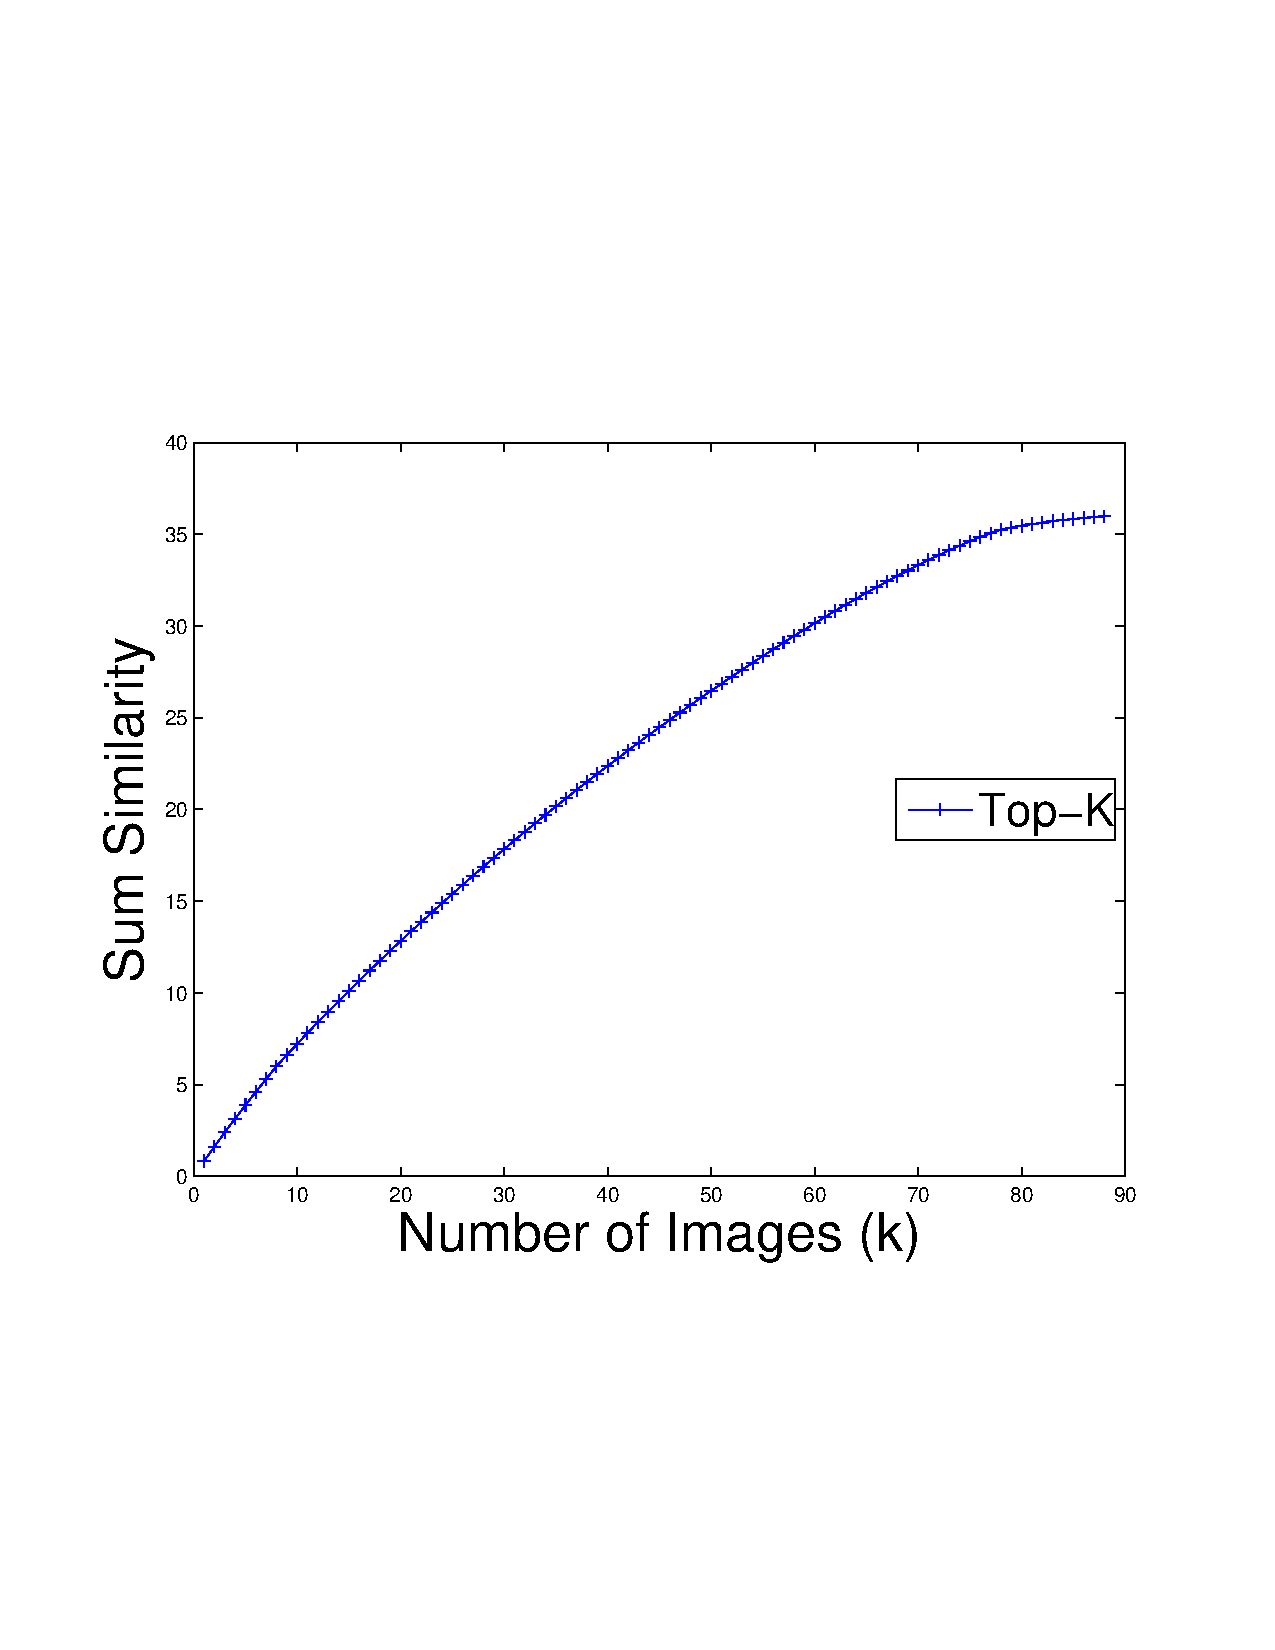
\includegraphics[clip=true, trim = 17mm 65mm 25mm 70mm, scale=0.23]{figures/topk/topk_sum_sim_color.pdf}
        \label{fig:topkSumSim}
        }
    \subfigure[Top-K: Avg. Match Target]{
        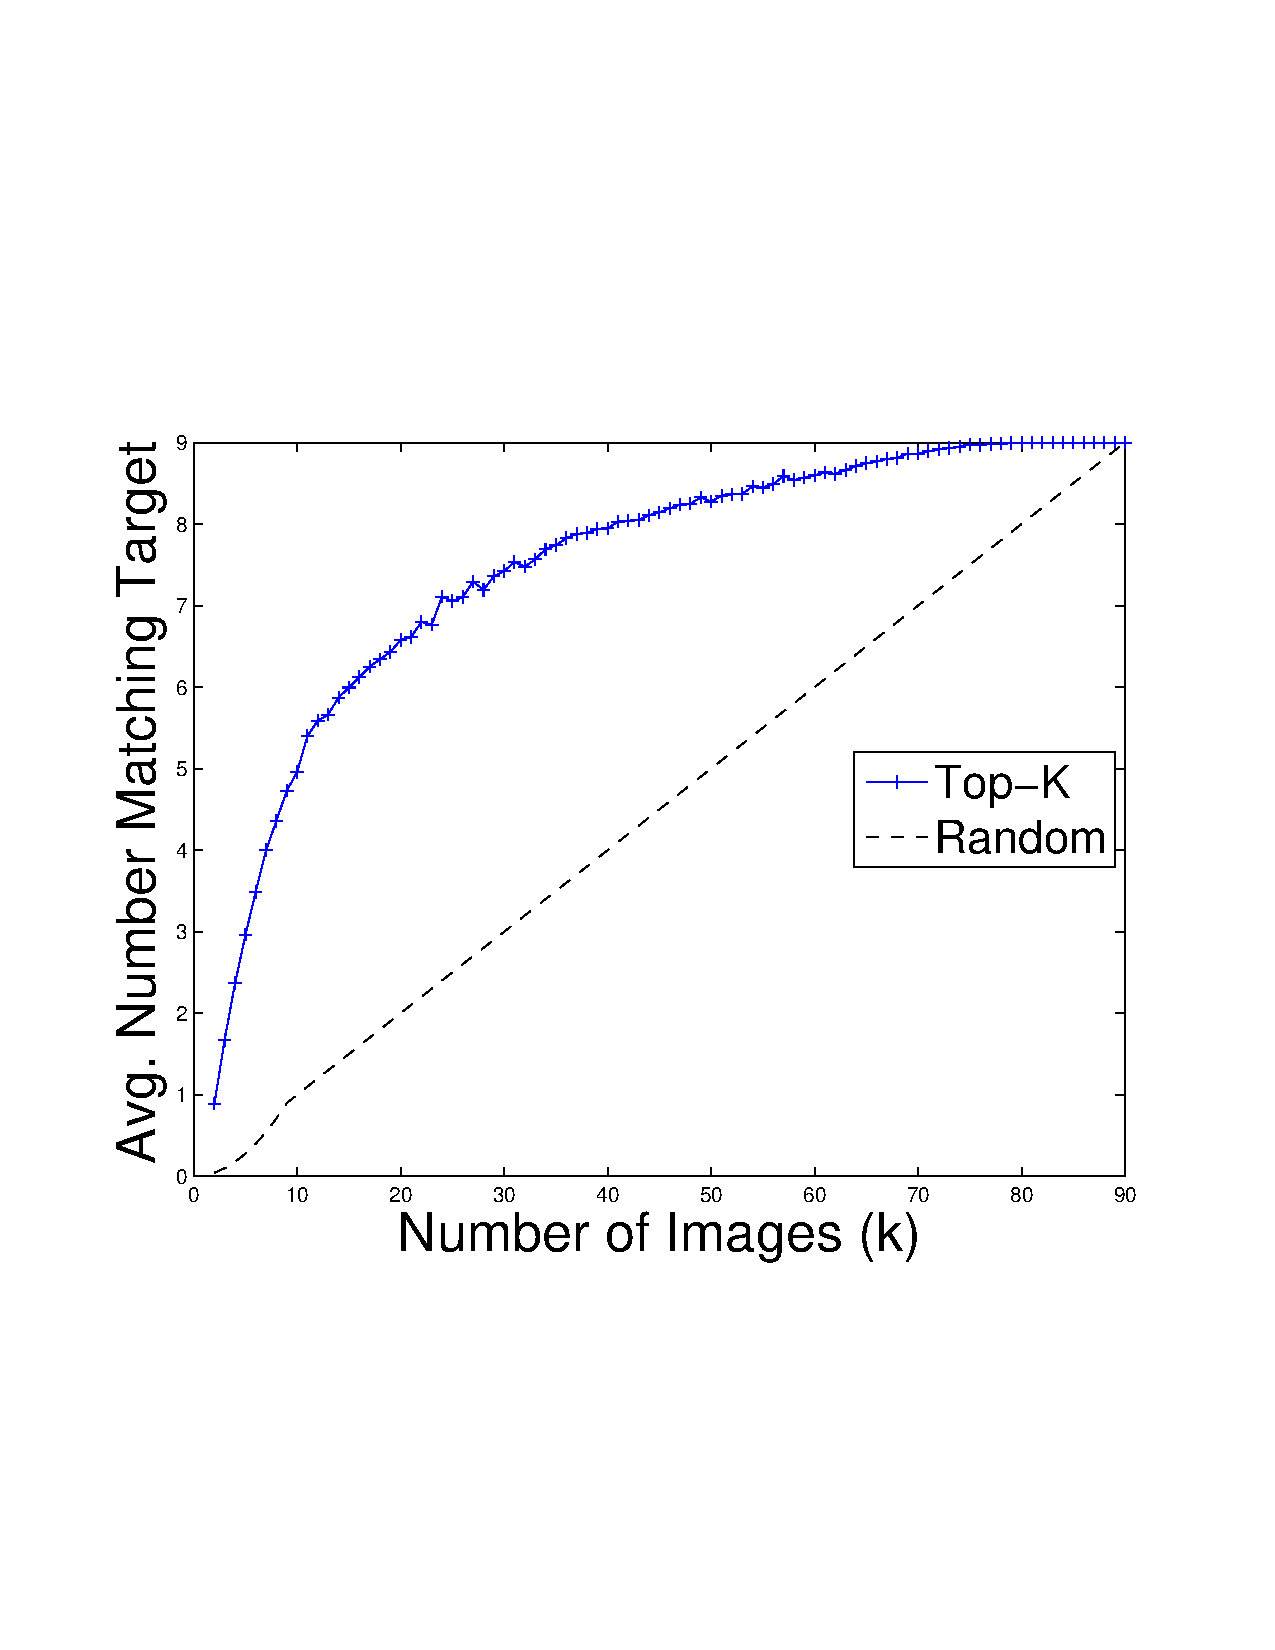
\includegraphics[clip=true, trim = 17mm 65mm 25mm 70mm, scale=0.23]{figures/topk/avg_num_matching_color.pdf}
        \label{fig:topkAvgNumSameSet}
        }
    \subfigure[Spanner: Sum Dissimilarity]{
        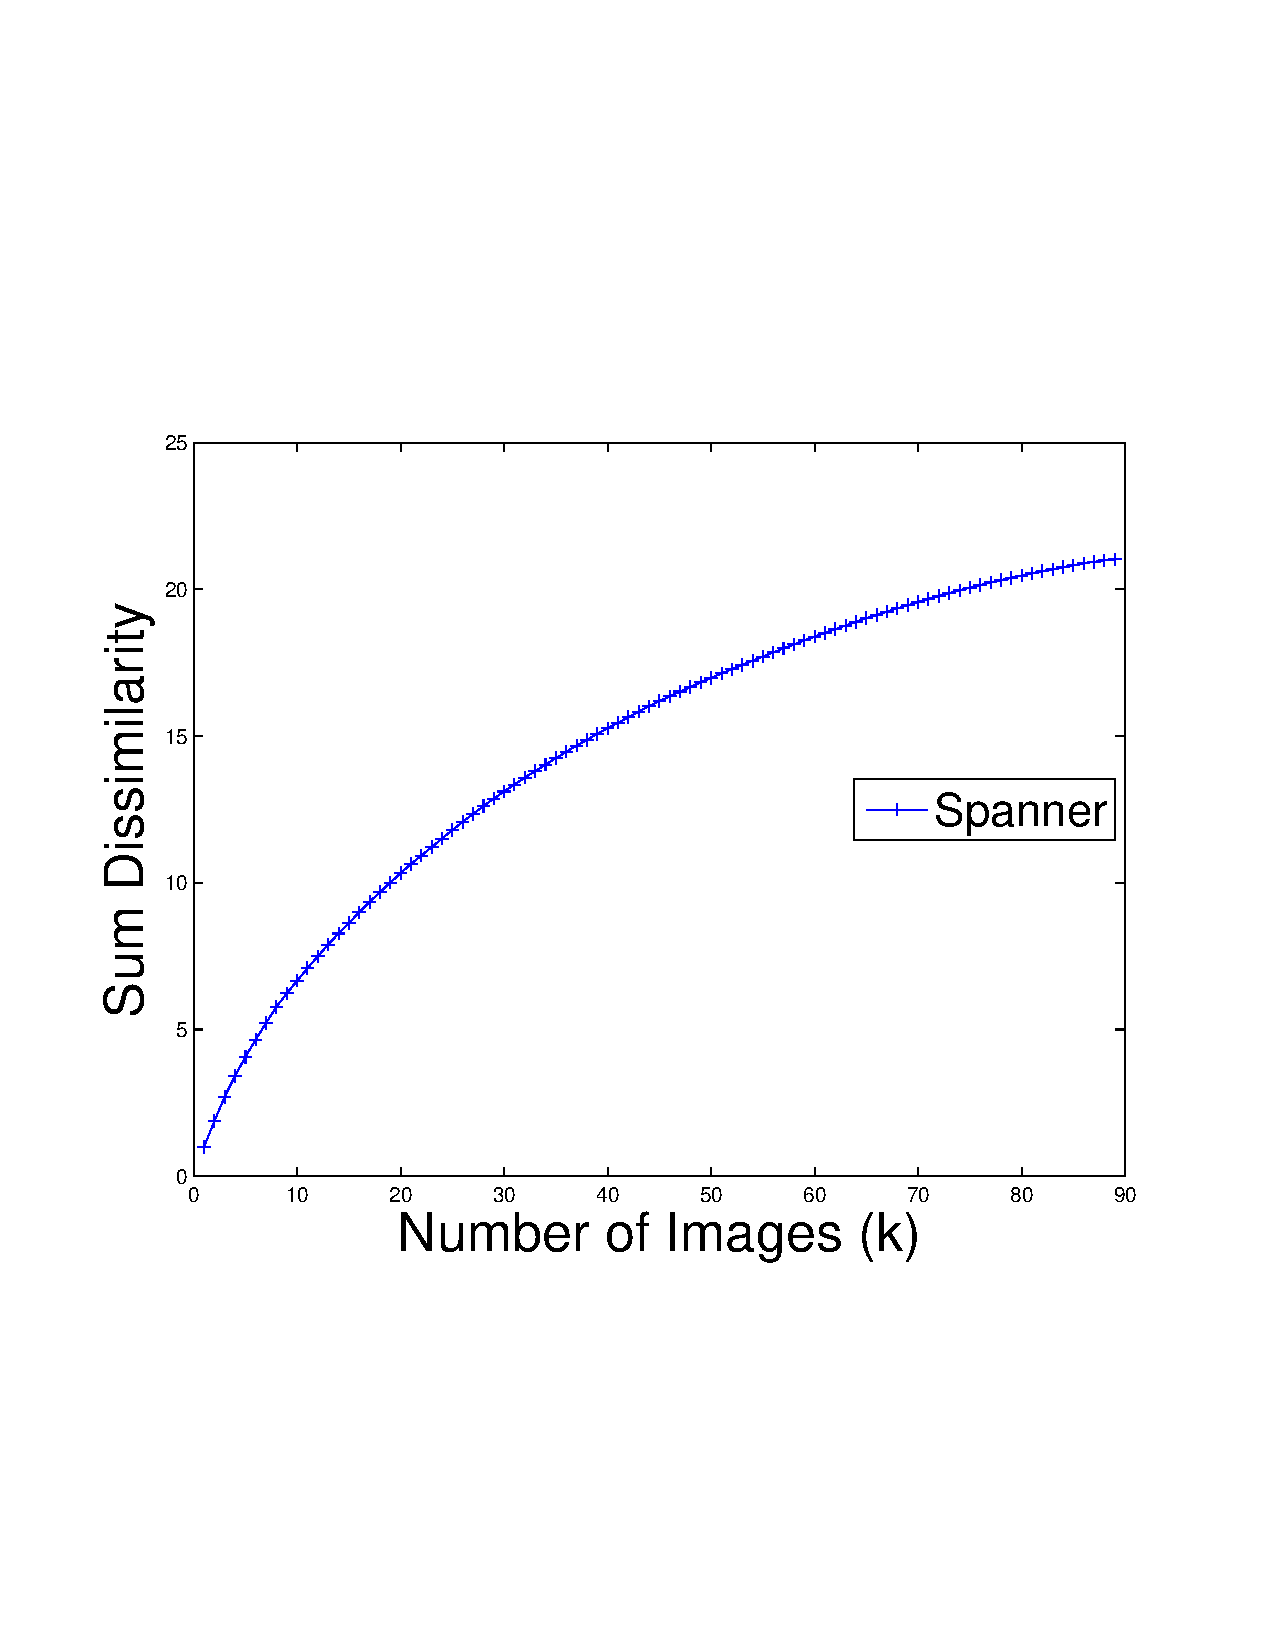
\includegraphics[clip=true, trim = 17mm 65mm 25mm 70mm, scale=0.23]{figures/spanner/spannerCumulativeDist_color.pdf}
        \label{fig:spanSumDissim}
        }
    \subfigure[Clustering: Cover All Sets]{
        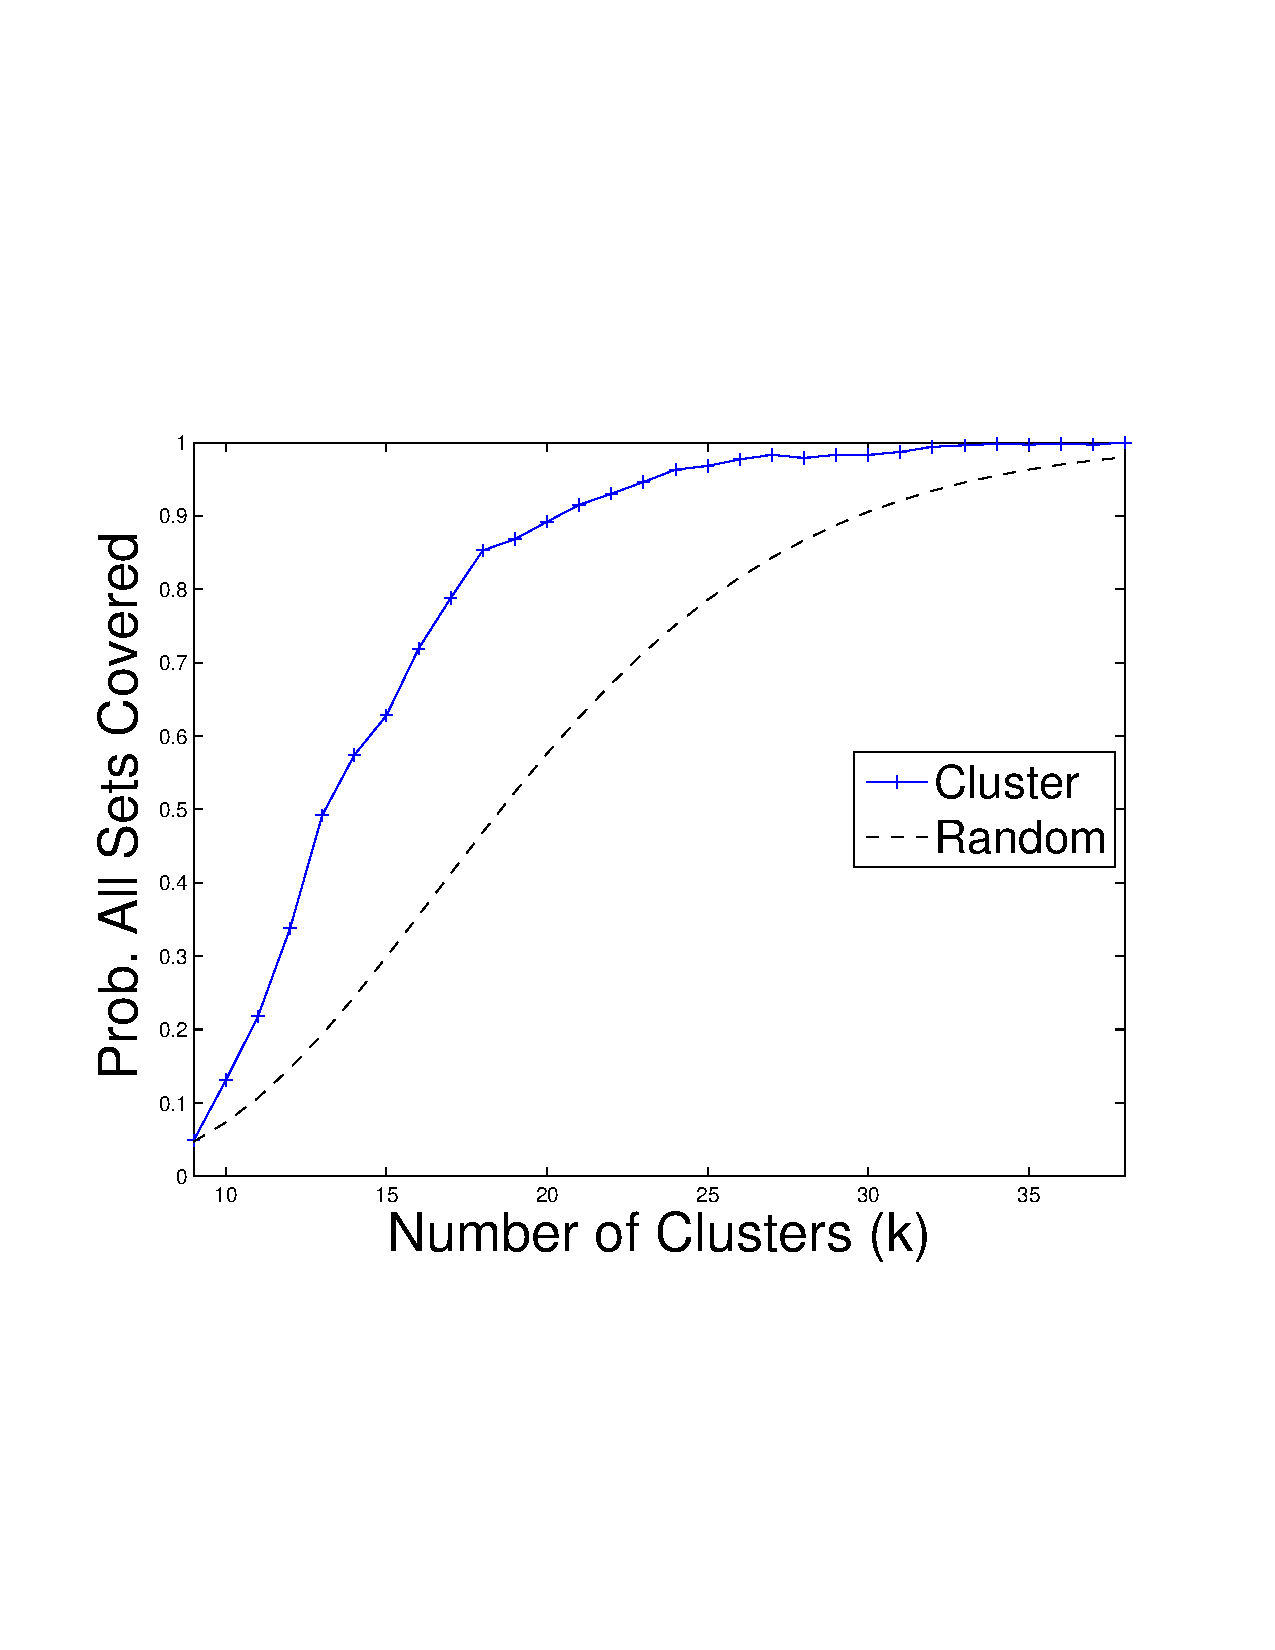
\includegraphics[clip=true, trim = 16mm 65mm 25mm 70mm, scale=0.23]{figures/cluster/perc_all_sets_covered_vary_k_color.pdf}
        \label{fig:clusterAvgNumSetsCov}
        }        
   \caption{Completeness metrics for the three image selection algorithms. Each exhibits a diminishing return as more images are added.}
   \label{fig:completeness_exp_results}
   \vspace{-4mm}
\end{figure*}

\section{QoI Model}
\label{sec:qoi_model}

%\begin{figure}
%\centering
%    \subfigure[Sum Similarity]{
%        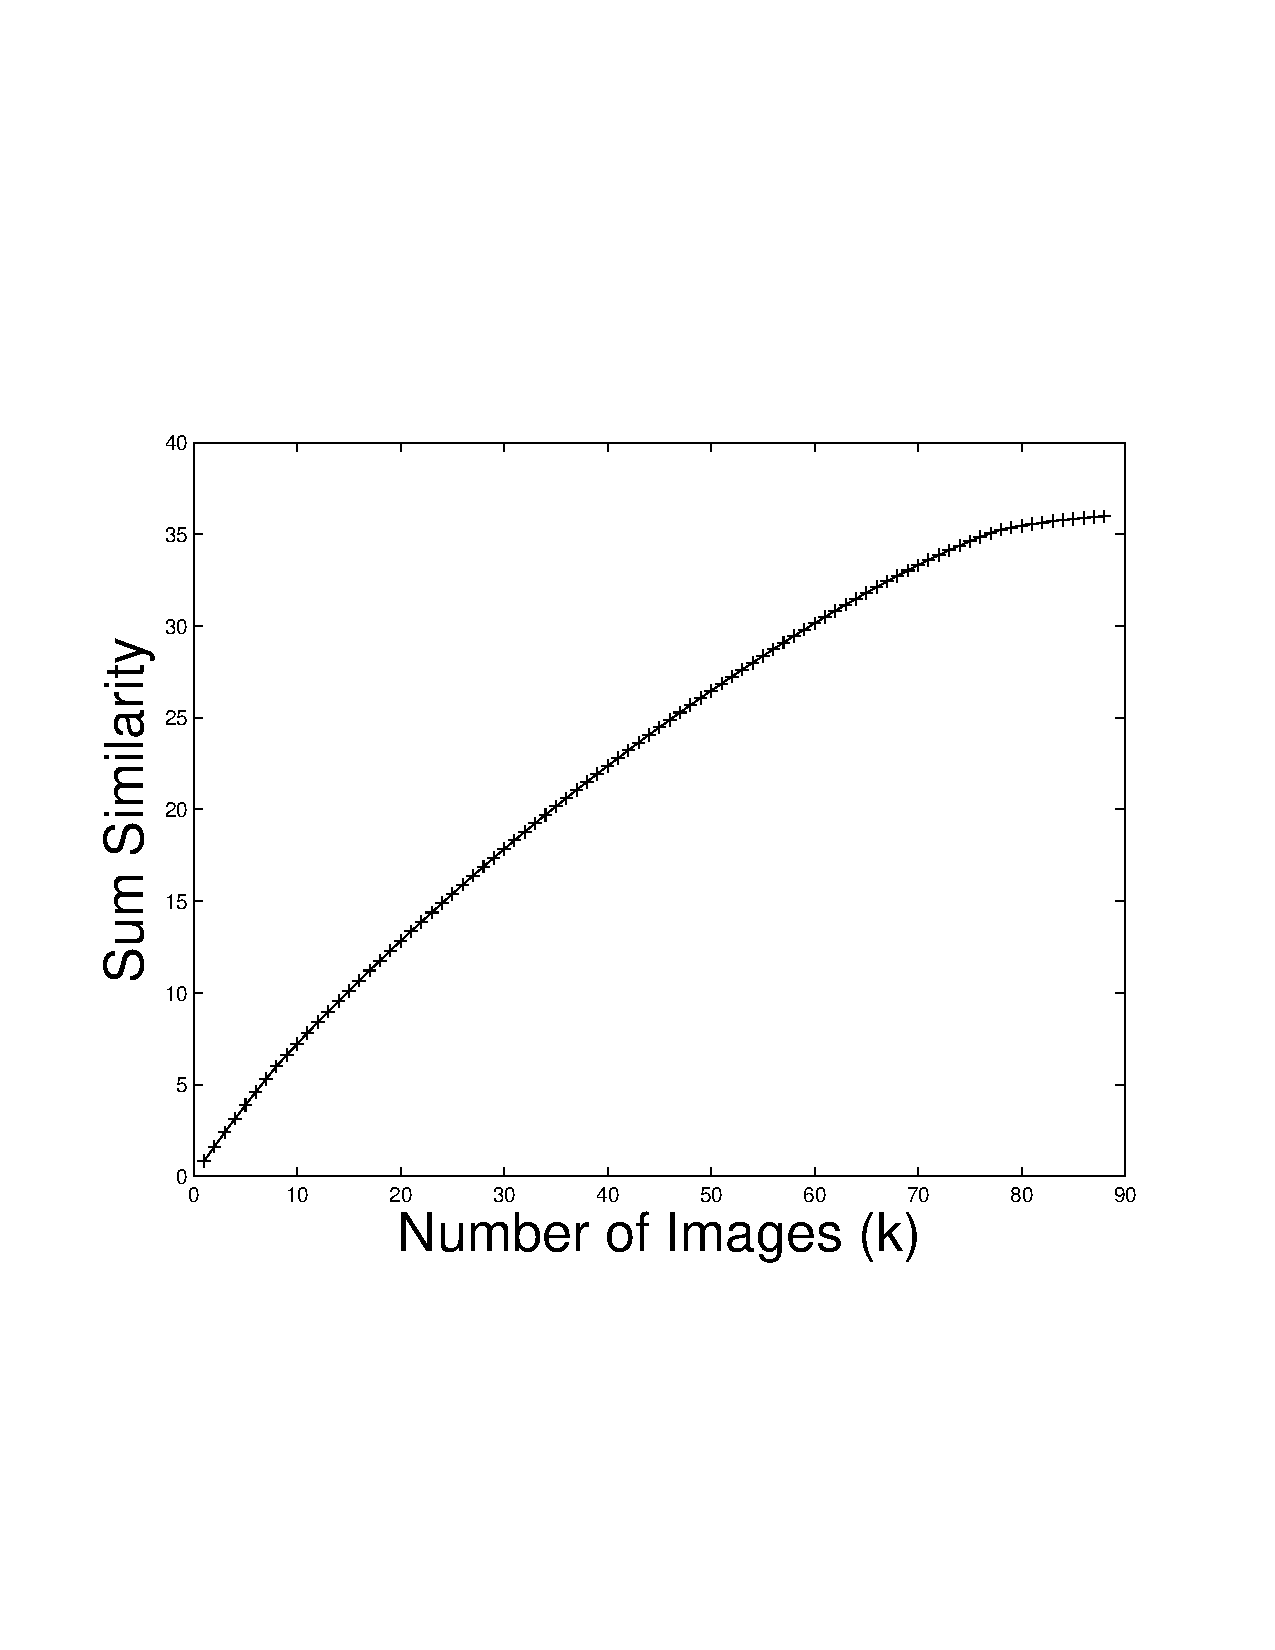
\includegraphics[clip=true, trim = 17mm 65mm 25mm 70mm, scale=0.23]{figures/topk/topk_sum_sim.pdf}
%        \label{fig:topkSumSim}
%        }
%    \subfigure[Avg. Match Target]{
%        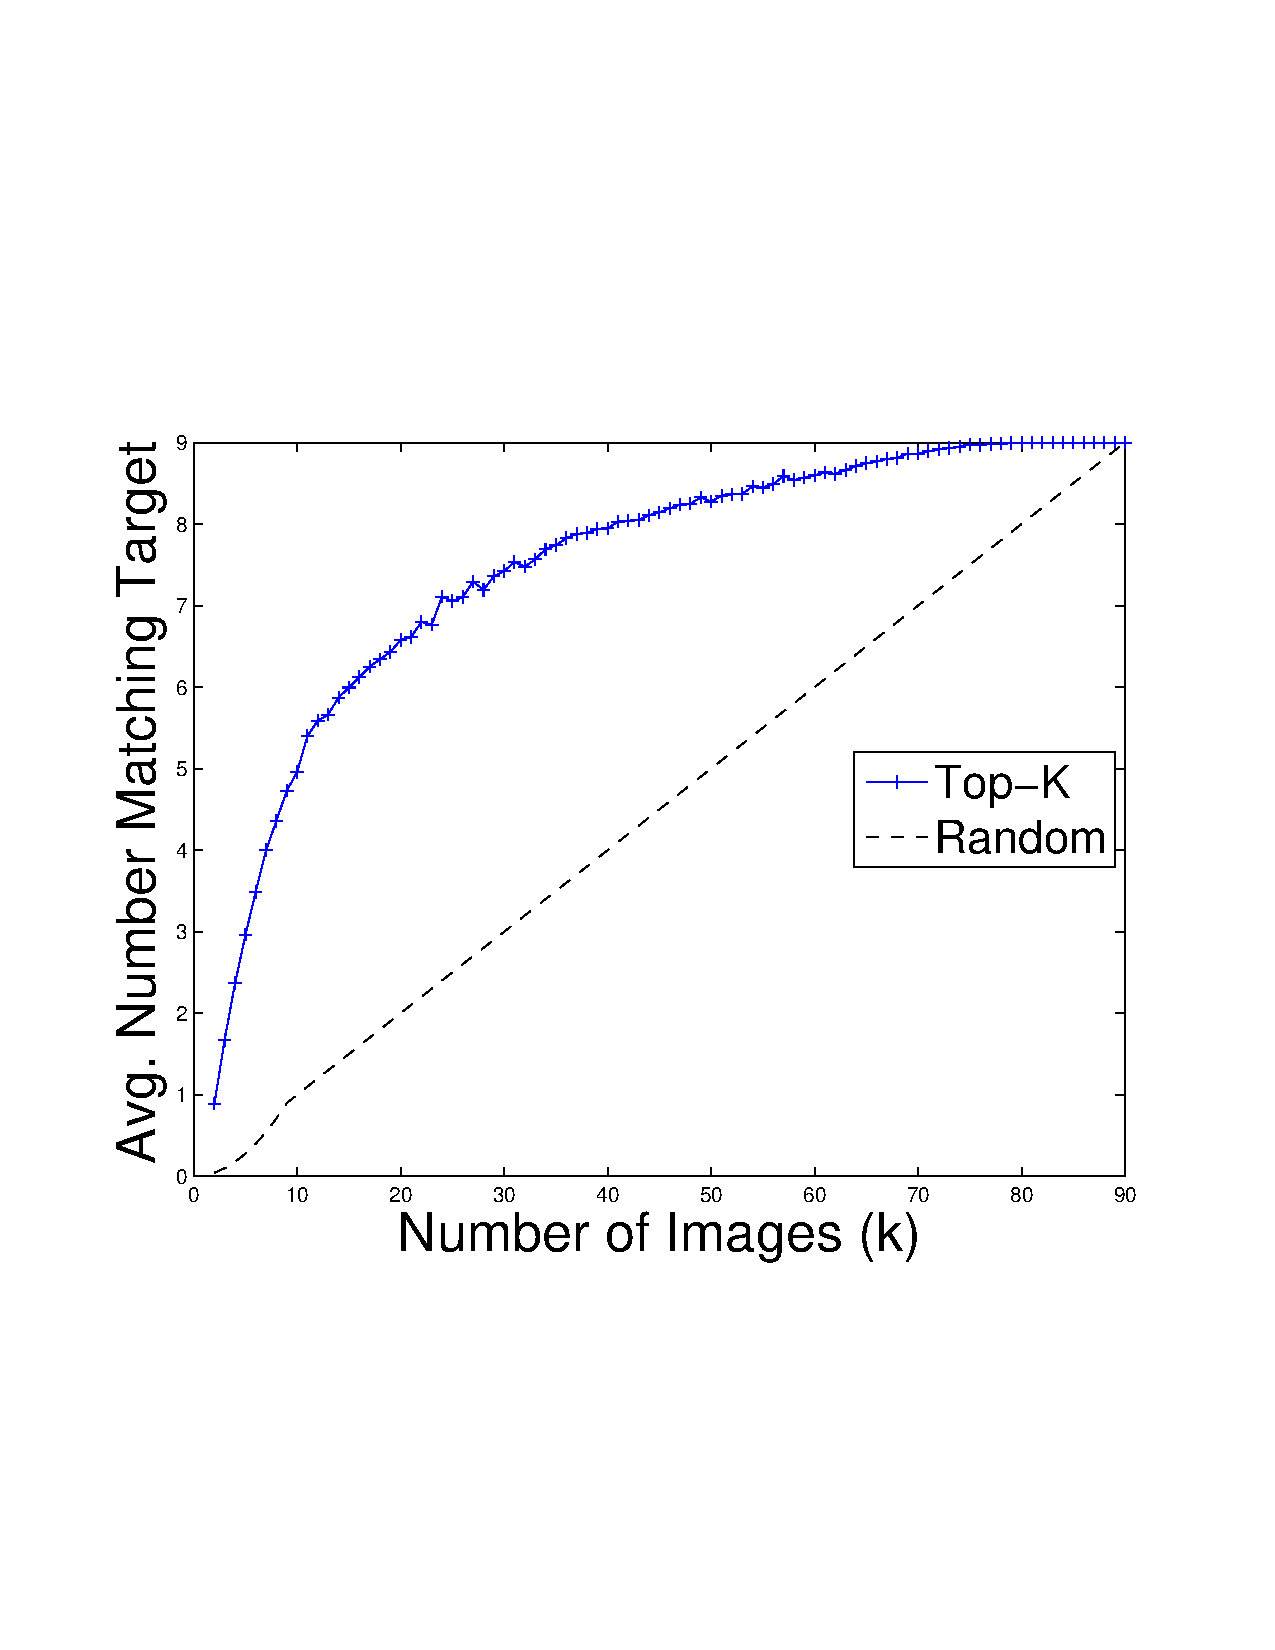
\includegraphics[clip=true, trim = 17mm 65mm 23mm 70mm, scale=0.23]{figures/topk/avg_num_matching_color.pdf}
%        \label{fig:topkAvgNumSameSet}
%        }
%   \caption{Completeness metrics for the Top-K selection algorithm. Each exhibits a diminishing return as more images are added.}
%   \label{fig:completeness_exp_results}
%\end{figure}

\begin{figure*}
\centering
    \subfigure[Top-K: Sum Similarity]{
        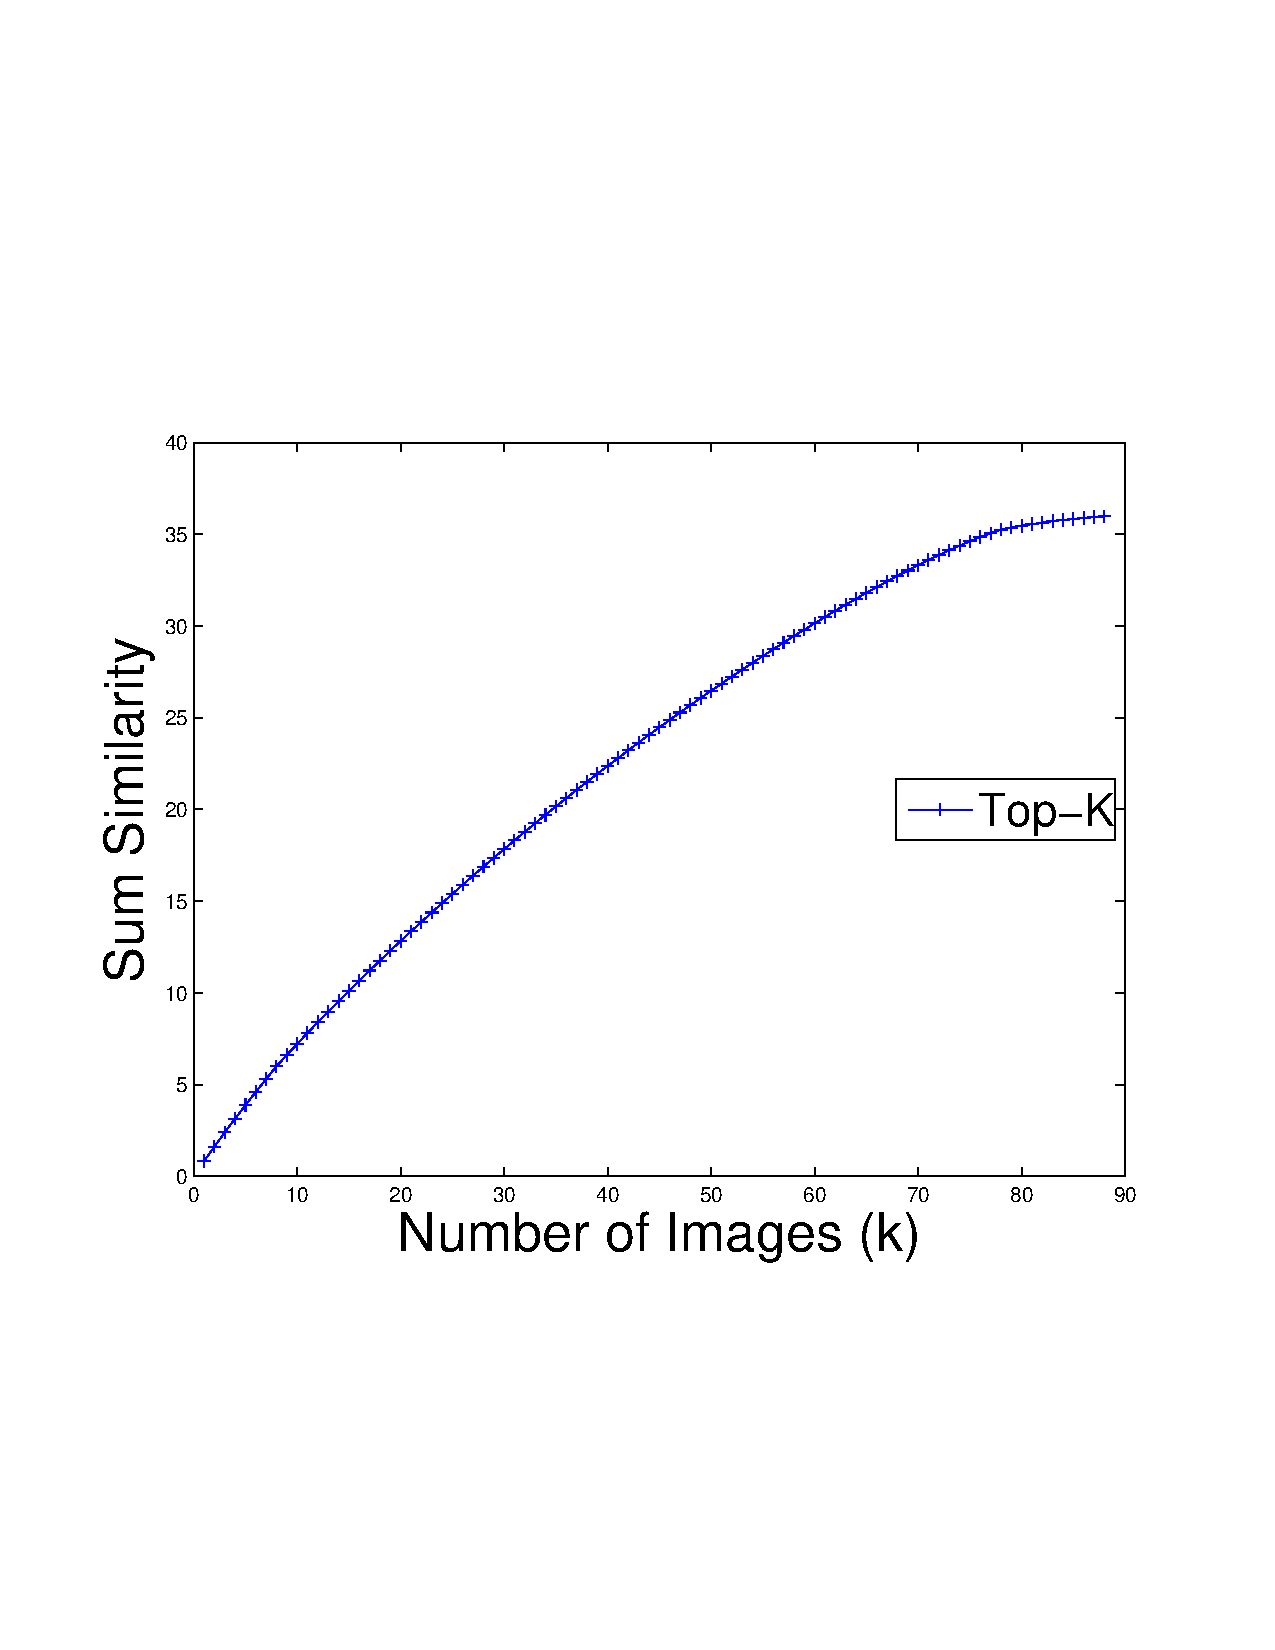
\includegraphics[clip=true, trim = 17mm 65mm 25mm 70mm, scale=0.23]{figures/topk/topk_sum_sim_color.pdf}
        \label{fig:topkSumSim}
        }
    \subfigure[Top-K: Avg. Match Target]{
        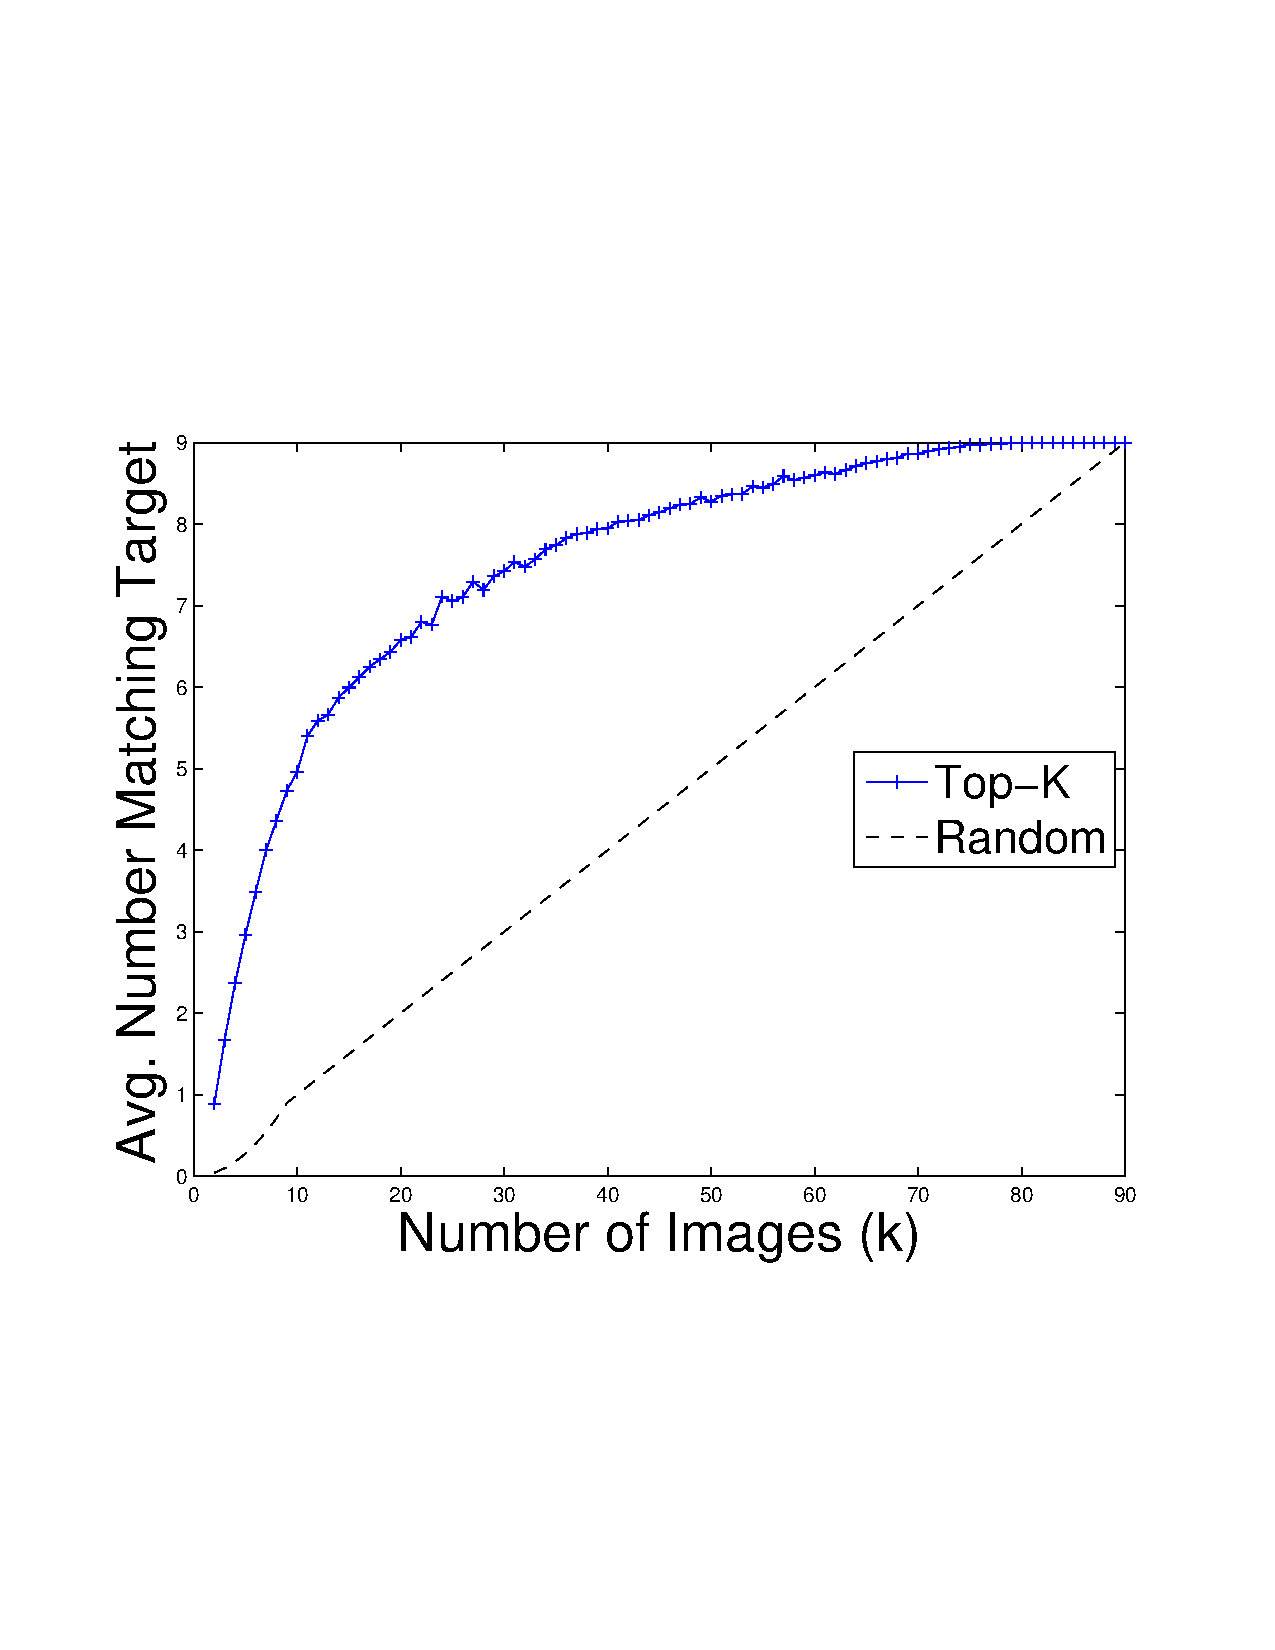
\includegraphics[clip=true, trim = 17mm 65mm 25mm 70mm, scale=0.23]{figures/topk/avg_num_matching_color.pdf}
        \label{fig:topkAvgNumSameSet}
        }
    \subfigure[Spanner: Sum Dissimilarity]{
        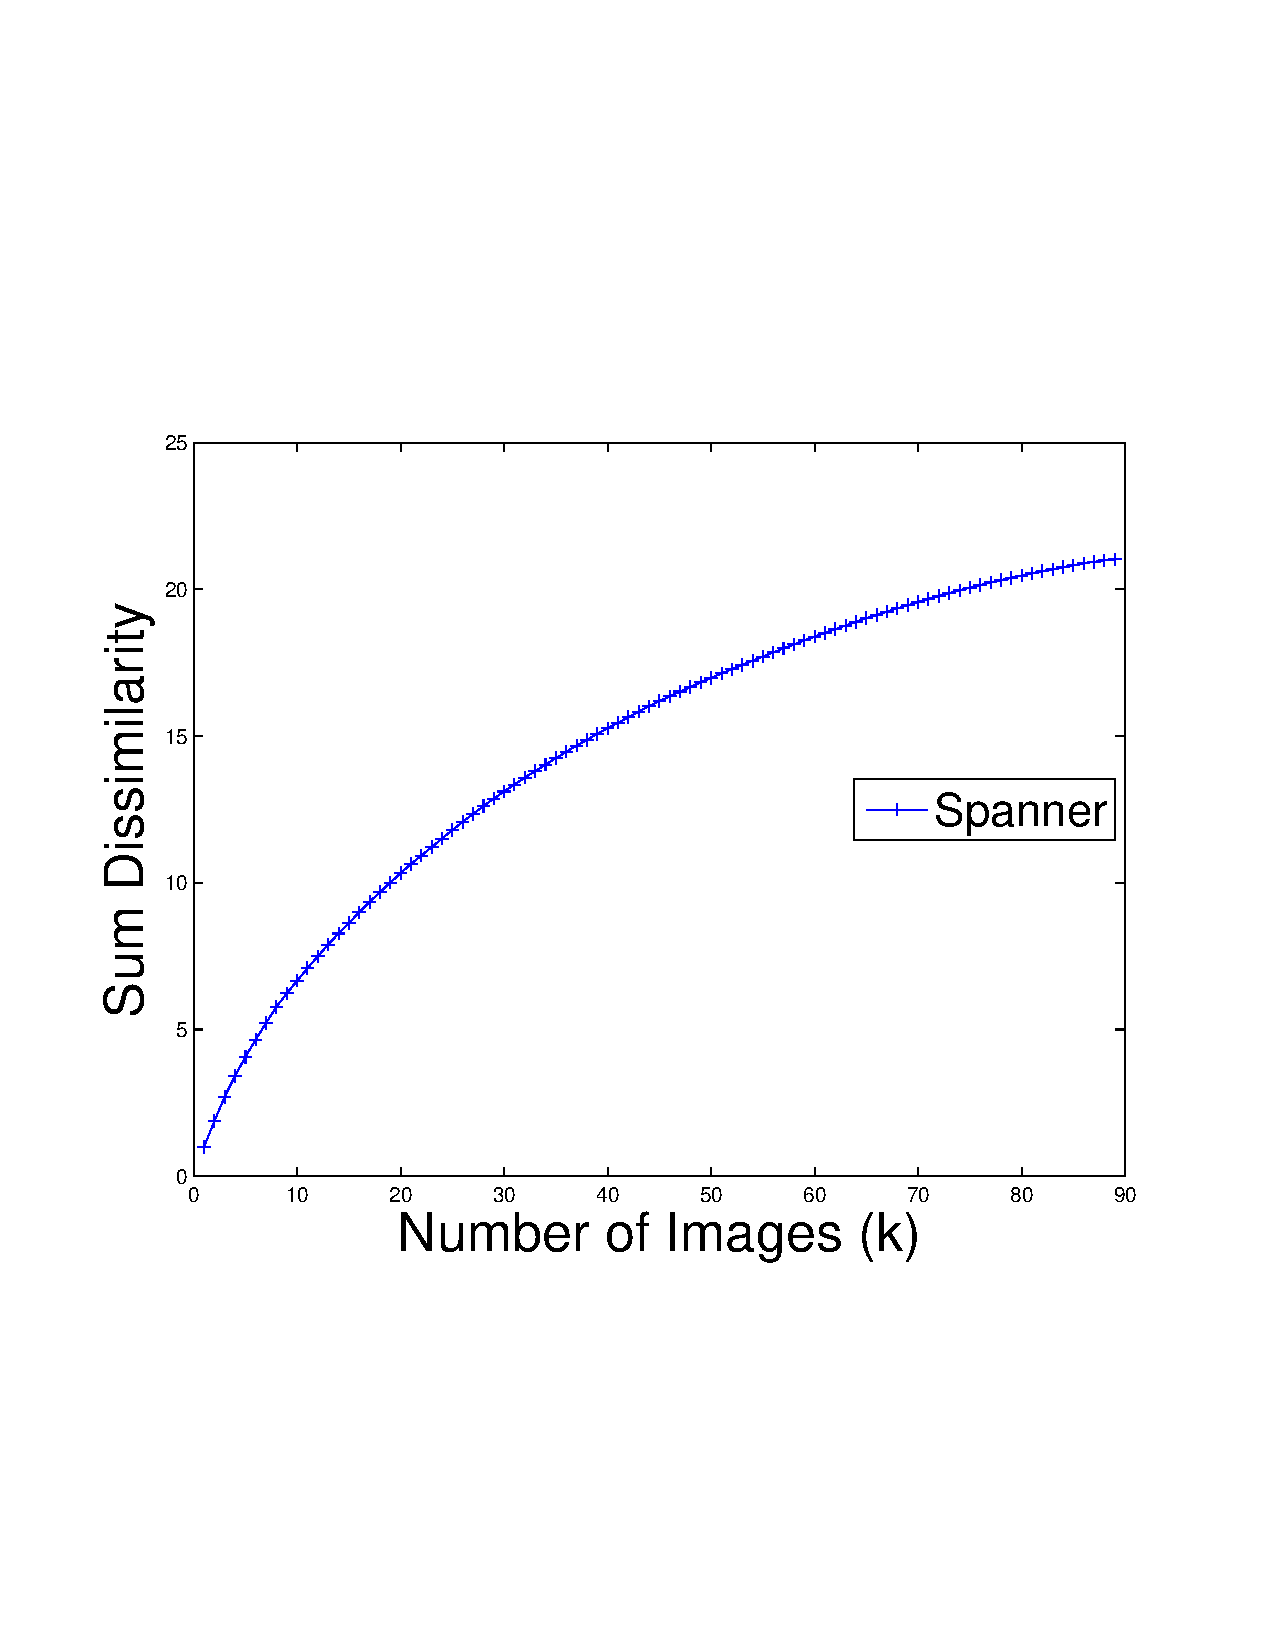
\includegraphics[clip=true, trim = 17mm 65mm 25mm 70mm, scale=0.23]{figures/spanner/spannerCumulativeDist_color.pdf}
        \label{fig:spanSumDissim}
        }
    \subfigure[Clustering: Cover All Sets]{
        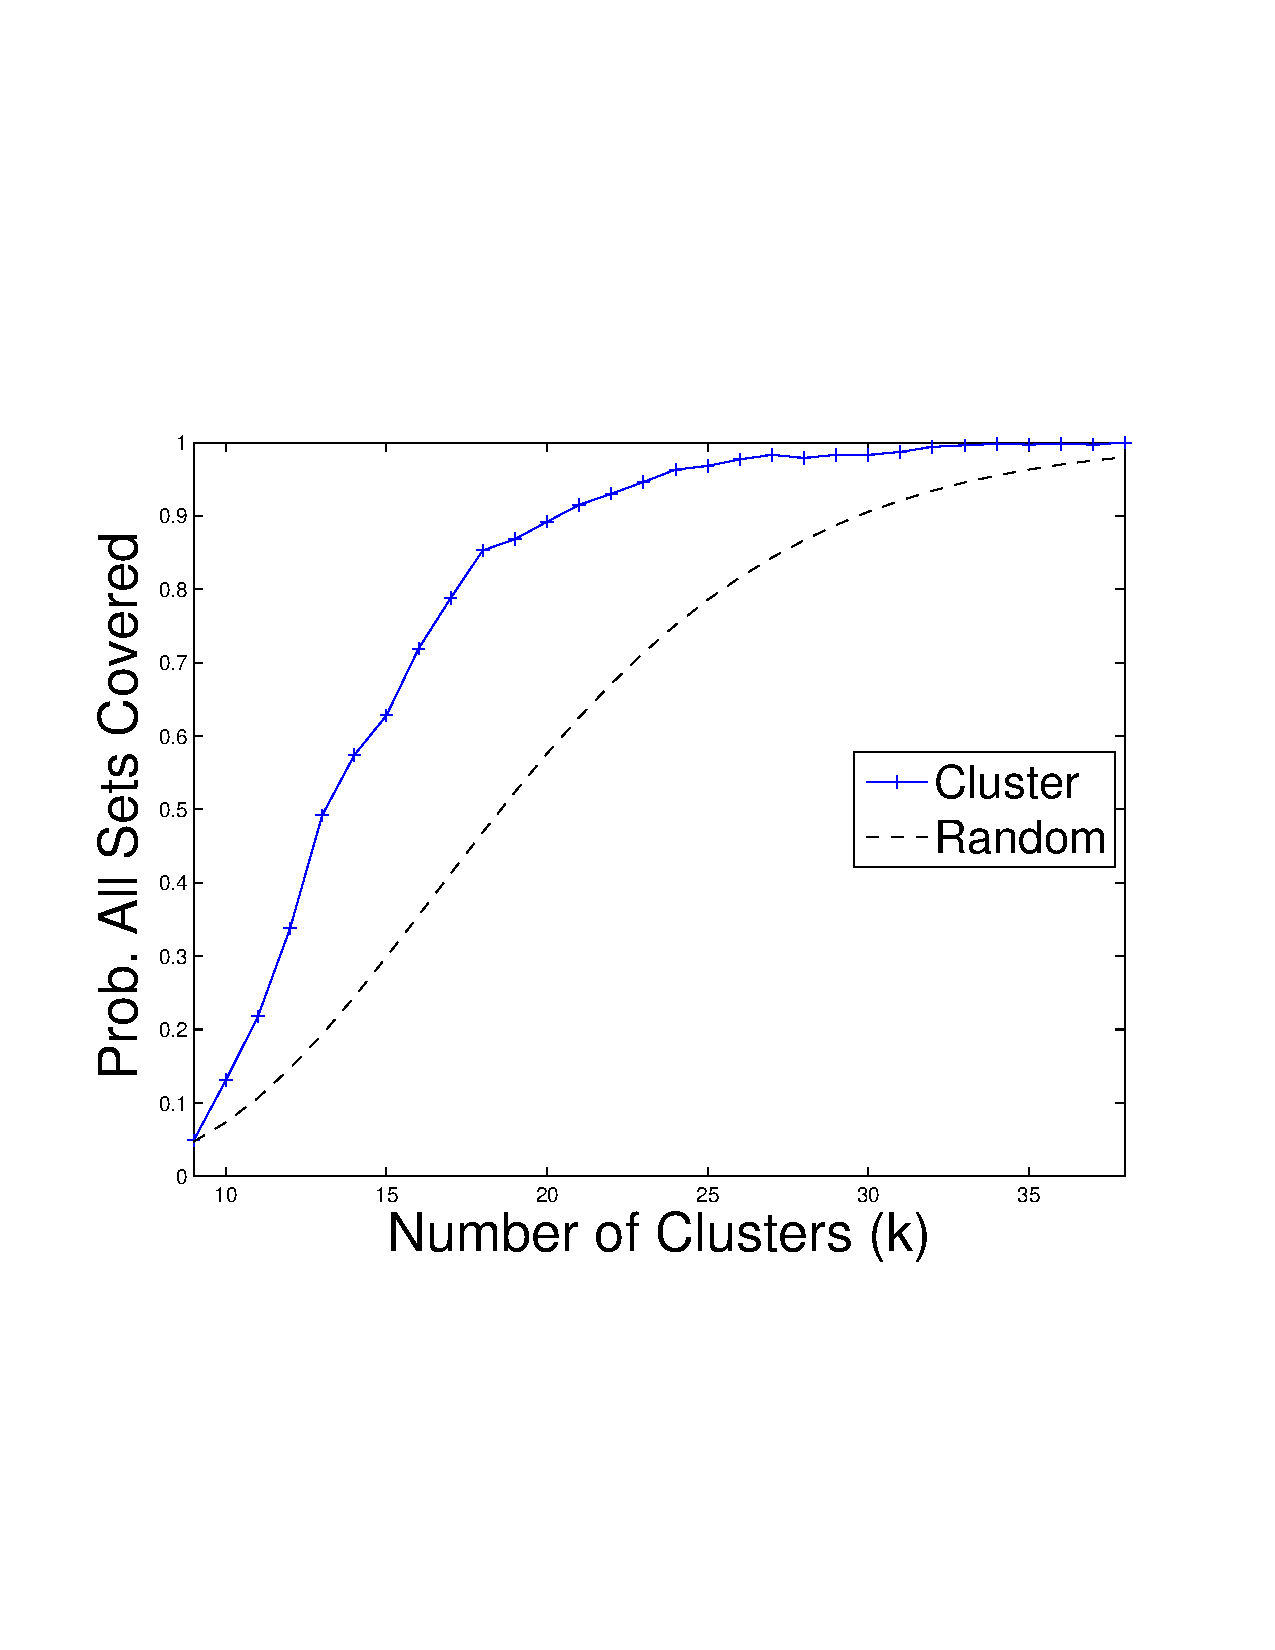
\includegraphics[clip=true, trim = 16mm 65mm 25mm 70mm, scale=0.23]{figures/cluster/perc_all_sets_covered_vary_k_color.pdf}
        \label{fig:clusterAvgNumSetsCov}
        }        
   \caption{Completeness metrics for the three image selection algorithms. Each exhibits a diminishing return as more images are added.}
   \label{fig:completeness_exp_results}
\end{figure*}

QoI is a multi-dimensional metric that can be defined for an application to give a more meaningful measure of the value of information.  It consists of attributes such as  timeliness, freshness, completeness, accuracy, precision, etc.  
For example, information that contributes to a decision-making process may only be useful if it arrives before the decision must be made, or it may have varying usefulness based on how similar or dissimilar it is to other data already collected.

The specific details of which attributes are considered and how they contribute to QoI is application-dependent.  Chosen QoI metrics are stored as a vector associated with a data item.  
Here, as in \cite{qoi_aware_tactical_mil_nets}, we specify a vector of minimum values for each QoI metric, and 
information is evaluated based on whether it satisfies all of the QoI requirements or not.  We use this approach to establish the edges of QoI satisfiability for the vector of metrics, which defines the boundaries of maximum achievable QoI regions in the metric space.

We choose to use two QoI attributes, one that is time-based and one that is information-content-based.  The first attribute is timeliness, $T$, of data.  For the second attribute, we present a notion of \emph{completeness}, $C$, which we show can be defined multiple ways, depending on the application and context.  Together, a QoI requirement of $\mathbf{q} = \{C,T\}$ specifies a quantity of data that must be delivered as well as a deadline by which it must arrive to be useful.  Since completeness is a rather new concept, we explain an example image selection algorithm and show how it can be evaluated with completeness.
%REFERENCES THAT USE COMPLETENESS: 1) mentions completeness of information in context of mobile sensor networks; argues that mobility can increase coverage/completeness \cite{qoi_data_collection_mobile_sens_nets};  

\subsection{Example Application: Similarity-based Image Retrieval}

As a motivating example, we choose a network in which nodes store photographs that are to be exchanged or collected at one or more data sinks.  This example covers surveillance missions of military tactical networks or camera sensor networks.  In this model, nodes can act as both clients and servers, issuing queries and serving images in response.  Therefore, as the network size increases, the amount of traffic is also likely to increase, but possibly disproportionately.  This fact exemplifies why the problem of characterizing the scalability limits for an instance is not straightforward.

To satisfy completeness of a query, we utilize measurements of the similarity or dissimilarity between pairs of images as explained in the rest of this section.  To get a similarity measurement, we use the same choice as was shown to be effective in \cite{mediascope}.  A technique called Color and Edge Directivity Descriptor (CEDD) \cite{2008cedd} provides a $54$-byte vector of qualities inherent to a photograph like lightness, contrast, and color.  The similarity between two images can then be given as a scalar by calculating the \emph{Tanimoto Similarity} \cite{tanimoto} between their CEDD vectors.  Dissimilarity is simply defined as $1$ minus the similarity.

\subsubsection{Selecting Similar Images}
One possible query for data is to retrieve images from the network that are similar to an identified target image.
The first type of query we introduce occurs when a user already has one image of a particular area or object of interest and would like to obtain similar images to get a more complete view of that specific scene or object.  
For example, if a user has a picture of an unknown suspicious person entering a building, but the person is not identifiable from that image, it would be useful to collect more images that are similar to that one with the possibility that another picture may have a better view of the person in question that can be used for identification or more context.  Called {\bf Top-K}, the query algorithm used for this application will choose the $k$ images with the most similarity with respect to the target image.  

We can evaluate the completeness of the result in one of two ways.  First, we can use the similarity of the images as a value representing each image's effectiveness in providing a more complete view of the target scene.  If we sum the similarity of all $k$ images returned by the algorithm, we get a representation of completeness, which we naturally call \emph{Sum Similarity}.  While this measure of completeness is abstract, it can be refined in an actual implementation through testing and evaluating.  This definition of completeness is useful, though, because it can be applied without any predetermined knowledge of the environment or pool of images.  

Often, though, we can partition the environment in which the network operates into a number, $n$, of distinct settings or areas.  In those cases, we can utilize a second method of quantifying completeness.  Assume that each image belongs to one of these $n$ sets, %$Q_i$, 
related to the setting it depicts.  Naturally, then, when executing a Top-K query, the goal is for the algorithm to return images from the same set as the target image.  Completeness can then be given by the fraction of images returned that are in the same set as the target image.

\subsubsection{Selecting Diverse Images}

In contrast, given the set of all photographs available in the network, we might want to return the set of $k$ images that exhibits the most diversity, ideally providing a user with a good sampling, or \emph{complete view}, of available images.  For instance, such a result would be quite useful in a surveillance mission.  We present two query algorithms that can be used to achieve this goal.

One query that provides diverse images is known as the {\bf Spanner} of the set of known photographs.  For the Spanner algorithm, we employ a greedy algorithm similar to that in \cite{mediascope}.  Here, the algorithm simply chooses images that provide the greatest minimum distance from all images already chosen.  This minimum distance can be added to a running sum to provide a completeness metric of \emph{Sum Dissimilarity}.  This value represents a measure of completeness because a higher level of dissimilarity provides a more complete view of the feature space.

%Here, the algorithm first chooses the two images with the greatest dissimilarity between them from all available images.  Then, each successive image is chosen to be the one with the greatest minimum distance between it and all images already chosen, until $k$ images are selected.  This minimum distance between the image being selected and the images in the collected set is the value added to the running cumulative completeness metric of \emph{Sum Dissimilarity}.  Since the Spanner algorithm's goal is to provide images at the edges of the available feature space, the Sum Dissimilarity represents a measure of its completeness because a higher level of dissimilarity is providing a more complete view of the feature space.

The other query that can achieve a complete view over all images is {\bf Clustering}.  In the Clustering algorithm, all images are separated into $k$ clusters based on their pairwise distances using any version of a k-means clustering algorithm, where $k$ is given by the user.  Then, the most central image from each cluster is returned.  
Here, assuming that the photographs of the same settings or objects of interest exhibit similar characteristics, 
Clustering also provides a complete view of the network's environment.

Both Spanner and Clustering algorithms can also be evaluated using a model assuming the environment is split into $n$ sets.  With this model, we can define completeness as either the number of sets represented by at least one of the $k$ images returned or the probability of all $n$ sets being represented by at least one image when $k$ are returned.  Here, though, we only show results for the second definition.

\subsection{Experimental Results}

To provide example values of these completeness metric definitions, experiments applying each query algorithm were run on a set of pictures taken at $n = 9$ different settings around the Penn State campus.  Each of these $9$ settings is of a pictorially different area, e.g. a particular building, a downtown street, or a lawn setting, and over $20$ images of each was taken.  Then, for individual trials, $10$ images from each set were randomly selected to create an image pool of $90$ pictures.  The three algorithms were run over these $90$ images, with the target image being randomly selected in the case of Top-K.  Results for each of the different completeness metrics were averaged over $1,000$ trials are shown in Figure \ref{fig:completeness_exp_results}. % Figures \ref{fig:topkSumSim} to \ref{fig:clusterAvgNumSetsCov}.

Figure \ref{fig:topkSumSim} shows the average sum similarity of images returned by the Top-K algorithm.  Figure \ref{fig:topkAvgNumSameSet} provides the second definition of completeness for the Top-K algorithm, the number of images matching the set that the target image was randomly chosen from.  Completeness results when dissimilarity is the objective are shown in Figures \ref{fig:spanSumDissim} and \ref{fig:clusterAvgNumSetsCov}.  Specifically, Figure \ref{fig:spanSumDissim} depicts the average Sum Dissimilarity returned by the Spanner algorithm, and Figure \ref{fig:clusterAvgNumSetsCov} represents the empirical probability of all $9$ sets being represented in the $k$ returned images.   For reference, we also include expected values for the metrics in Figures \ref{fig:topkAvgNumSameSet} and \ref{fig:clusterAvgNumSetsCov} if the images were selected from the entire image pool at random, i.e., without regard for image similarity or dissimilarity.  Details on these expected values given random selection are in Appendix \ref{sec:expl_exp_qoi}.

These figures exhibit the diminishing returns of completeness as more images are collected.  This effect visually shows how QoI differs from throughput.  As seen in these graphs, transmission of successive images does not result in a linear gain in completeness.  For example, in Figure \ref{fig:topkAvgNumSameSet}, it is evident that a value of only $k \approx 10$ is needed to collect $5$ images matching the target content, while collecting an additional $2$ from the same set usually requires collecting over twice that number of pictures.  
%For comparison, Figure \ref{fig:topkAvgNumSameSet} also shows the completeness achieved by random selection.
Similarly, Figure \ref{fig:clusterAvgNumSetsCov} shows that jumping from $k=10$ to $k=20$, the likelihood of capturing at least one image of every setting grows substantially from just over $10\%$ to approximately $90\%$.  To approach probabilities close to gaining that final $10\%$, however, requires a jump to $k\approx30$.  

The relationship between the number of images and completeness in each of these graphs also shows that obtaining a certain value of QoI or completeness requires a different number of images depending on the set available and their similarities.  We can denote the number of images required to achieve a level of completeness, $C$, as $k_{req} = Q(C)$.  This relationship will be useful later in determining capacity and scalability limits.

%\subsection{Other Applications}
%In our work, we also studied and experimented with two other algorithms in \cite{mediascope} that provide completeness by returning images that are dissimilar from each, providing a representative view of available data.  These completeness definitions resulted in very similar relationships as seen in Figure \ref{fig:completeness_exp_results} and are omitted for space.  We also note that the formulation in Section \ref{sec:qoi_scalability} is not restricted to just completeness, but can be used with any QoI metric that can be translated into a data requirement.
\subsection{Further Discussion of QoI}
We have defined and provided examples for a number of ways that completeness can be defined and used to obtain a concrete data requirement from a contextual QoI requirement.  Throughout the rest of the paper, we use sum similarity and the probability of covering all sets using clustering as completeness metrics, but we note that any of the definitions of completeness used here, or any other QoI requirement that can be translated into a data requirement, for that matter, can be used. % in the formulation in Section \ref{sec:qoi_scalability}.

%Also, note that QoI and its usage in understanding networks is not exclusive to these metrics and applications.  On the contrary, the model used in the capacity and scalability analysis of Section \ref{sec:qoi_scalability} is meant to be an in-depth example of this concept.  Modifications to account for different data size requirements should be quite straightforward, and extensions to other time-based metrics should be possible with careful extensions to the framework.

Also, while metadata associated with photographs may be useful in obtaining similar goals to those given in this section, relying on such information is problematic because metadata is not guaranteed to be available, and it is not as universally applicable as content-based retrieval.  For example, tags describing the image contents would require users to participate by entering this information, which is time-consuming and unreliable.  Location and time stamps may be automatically applied by the device allowing an application to filter images accordingly, but these tags often do not account for factors such as the direction of the camera or obstructed views.  Content-based processing, though, can be applied to any set of images.





\section{QoI Scalability}
\label{sec:qoi_scalability}

Given the nonlinear returns of completeness and importance of timeliness outlined in the previous section, we contend that establishing limits of throughput is insufficient.  A non-QoI-aware approach ignores very useful information such as how changes in achievable data rates affect the actual utility of information at its destination as well as how changes in one QoI requirement can affect satisfiability of other requirements.  

For these reasons, we set the goal of determining the capacity of a network, and relatedly, the scalability achievable with respect to QoI requirements.  Previous methods that predict scalability do so by singling out a single bottleneck node and determining when it will be overloaded and drop packets. Here, we are forced to look at end to end flows and determine all contributors to delay, including MAC access, queuing delays, and multi-hop propagation to find the point at which timeliness requirements are violated or traffic load must be reduced thus adversely affecting completeness, leading to a more comprehensive analysis.

\subsection{QoI Satisfiability Framework}
In order to establish the framework, we examine an arbitrary flow, $F_1$, in the network that has a QoI requirement of $\mathbf{q} = \{C, T\}$, where $C$ is the minimum required completeness metric of choice, such as sum similarity as explained above, and $T$ is the required timeliness.  This flow will have a data size requirement, which is given by a chosen QoI function $Q(C)$.  Using the example application from \ref{sec:qoi_model}, for example, $Q(C)$ can return the number of images, $k_{req}$, required to achieve the requested completeness $C$. For simplicity, in this section, we use a fixed value for the data size requirement, but we expand our consideration to use a distribution for the data size requirement in our applications in Section \ref{sec:example_applications}.

Assuming each image has a size of $I_S$, then we can also use $B$ to describe the total number of bits required by the flow, $B=k_{req}*I_S$.  To match realistic network implications, we assume this data will be transmitted in a series of packets with size $P_S$ bits each. This packet size should include any bits necessary to implement techniques of error detection or correction that the network is utilizing. The number of packets per flow, then, is simply $P_N = \lceil B/P_S \rceil$.  We assume that each node in the network can transmit at $W$ bits per second when it is allocated media access.

Our goal is to establish the limits at which this arbitrary flow can no longer be completed with the QoI requirements satisfied.  {\color{blue}We build and explain our model for achieving this goal by working through an example TDMA line network, a portion of which is shown in Figures \ref{fig:delay_expl_fig_3} and \ref{fig:delay_expl_fig_4}. In this network, we assume a simple 3-slot TDMA scheme, which allows each node equal time access to the medium and, in this explanation, we remove any potential interference or hidden terminal issues. Recall that packet losses and retransmissions can be captured in this framework by using an \emph{effective} channel rate based on the physical channel rate and loss probability. Also, we discuss addressing non-TDMA networks, such as those that use a CSMA protocol, in Section \ref{sec:discussion}. }

The TDMA Slot assignments are labeled above each node in Figures \ref{fig:delay_expl_fig_3} and \ref{fig:delay_expl_fig_4}.  For simplicity, we will assume that one slot is appropriately sized to transmit a single packet, i.e., $T_{slot} = P_S/W$ and that packets use static routes calculated beforehand such that the overhead is not a consideration here.

{\color{blue}When calculating overall delay, four sources of delay are generally considered: processing, queuing, transmission, and propagation. We focus on transmission and queuing delay here and ignore processing and propagation delay, because the latter two are negligible compared to the former two for the wireless channel rates we are targeting in this work (on the order of MBs/sec or lower). If a higher level of precision is desired, however, propagation and processing delays can be added to the time to transmit each packet, which we adopt as the time duration of a time slot, $T_{slot}$ below, without changing the formulation of the framework. Furthermore, we do not incorporate consideration of excessive queuing delays since, as we stated in the model, our aim is to evaluate stable network traffic, which implies relatively small queue backlogs. %, and cases in which traffic is causing high queueing delays will not be providing timely delivery of data, and, thus is also out of the scope of this work.

%Similarly, delays associated with processing of packets may be added to this emission delay. We also ignore these delays here, though, and assume that packets can be just forwarded with a minimal amount of processing, e.g., only decoding the header to determine the next hop.

In developing our framework, we find it more intuitive to split the total delay into two functional parts, which we call $D_1$ and $D_2$. These two components do not separate queuing and transmission delays, but considering parts of each simultaneously. }
%We split the components of delay that contribute to the total delay of completing flow $F_1$ into two parts, $D_1$ and $D_2$. Each of these components capture part of the queuing delay and part of the transmission delay. 
The first contributor, $D_1$, is the end to end delay incurred by sending the $B$ bits across the designated path in the network. To quantify this delay, we must consider several factors beyond just the available bandwidth and number of packets in a flow. First, each node must share the channel with its one-hop neighbors, creating a factor of delay inversely proportional to the percentage of time access that it is allocated for a channel. We call this factor of delay the Channel Factor, which in this case is given by $CF = N_{frame}/N_{i}$, where $N_{i}$ is the number of slots allocated to node $i$ and $N_{frame}$ is the total number of slots in each frame. In this case, $N_{i} = 1, \forall i$ and $N_{frame} = 3$. 

The second factor to consider for $D_1$ is the fraction of allocated slots that are utilized by the node to serve flows other than $F_1$ that are either originating in or being routed through nodes on the path of flow $F_1$.  We call the total number of flows competing at node $i$ the Traffic Factor, $TF_i$, of that node.  For any flow, the maximum contributor to delay is the node along the path with the maximum $TF_i$, which we will just call $TF$ here.  More detail about determining this $TF$ is outlined in Appendix \ref{sec:derivation_TFs}.  Incorporating these considerations into a calculation for $D_1$, we achieve the following expression:  % NOTE: Maybe want to add a max-flow, min-cut argument here to help clarify?
\begin{equation}
	D_1 = T_{slot} \cdot P_N \cdot CF \cdot TF
\end{equation}

\begin{figure}
\begin{centering}
    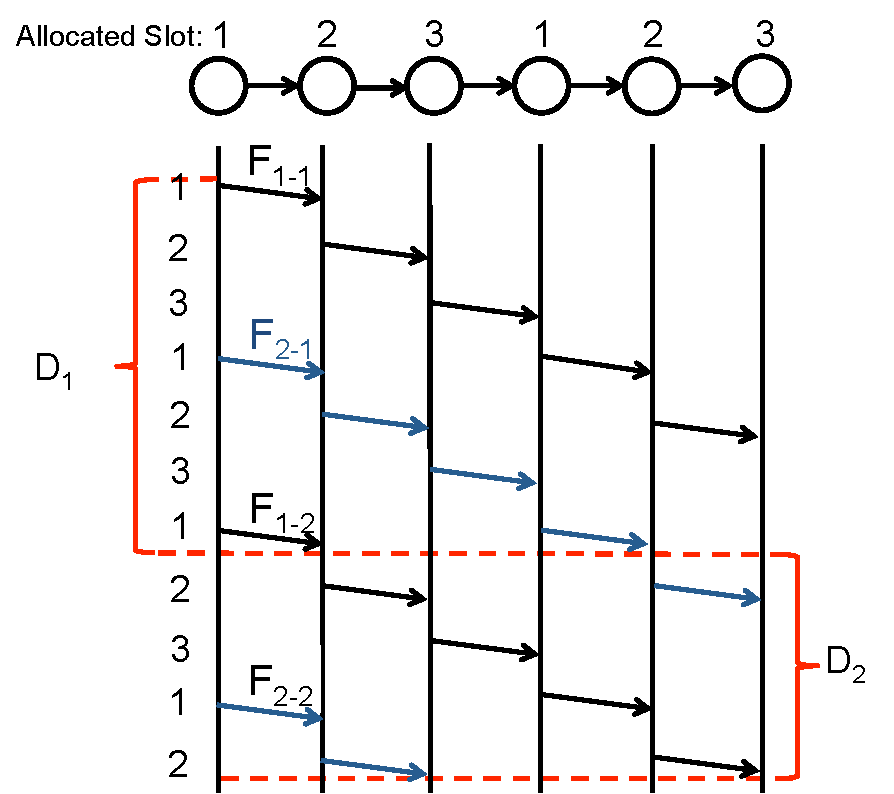
\includegraphics[scale=0.33]{figures/delay_limit_expl/fig_1_2.pdf}
    \caption{Example of line network using TDMA highlighting source of delays, $D_1$ and $D_2$.  (Node labels are slot assignments.)  Here, $TF = 2$, $CF = 3$, and $DF = 1$. }
    \label{fig:delay_expl_fig_3}
    \vspace{-6mm}
\end{centering}
\end{figure}

Figure \ref{fig:delay_expl_fig_3} depicts the delay of $D_1$ in a simple case of only two flows, $F_1$ and $F_2$, being present, in which case $TF = 2$.  In this example we use flows that consist of only $2$ ($F_{i-j}$ is packet $j$ in flow $i$) packets to portray the delay.  In most real applications, $P_N$ will be much larger, making $D_1$ a good approximation of this delay component.

\begin{figure}
\begin{centering}
    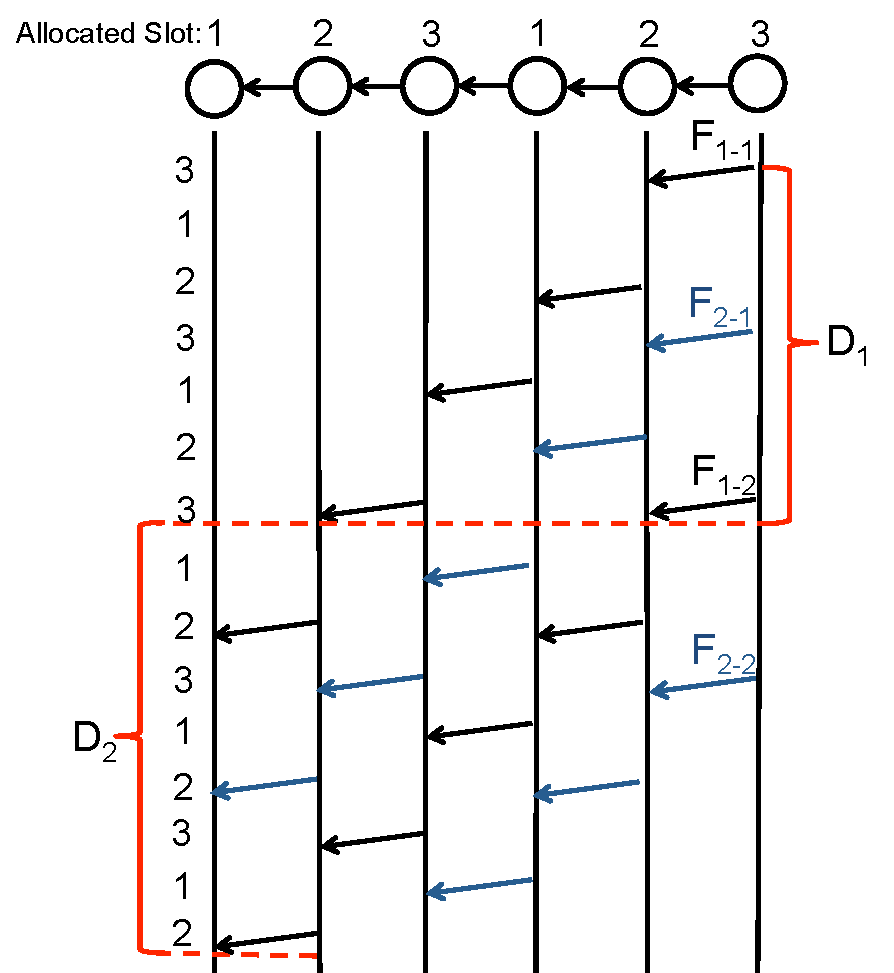
\includegraphics[scale=0.35]{figures/delay_limit_expl/fig_2_2.pdf}
    \caption{In the opposite direction, $DF = 2$. ($TF$ and $CF$ are unchanged here.)}
    \label{fig:delay_expl_fig_4}
    \vspace{-6mm}
\end{centering}
\end{figure}



\begin{table*}[]
\centering
\begin{tabular}{l|l|l|l|l|l|}
\cline{2-6}
%                            					 & \boldmath{$CF$}  			& \boldmath{$TF_{\mu}$}   			& \boldmath{$TF_{\sigma}$}										& \boldmath{$DF$}			& \boldmath{$PL_{max}$}	\\ \hline
                            					 & \boldmath{$CF$}  			& \boldmath{$\mu_{TF}$}   			& \boldmath{$\sigma_{TF}$}										& \boldmath{$DF$}			& \boldmath{$PL_{max}$}	\\ \hline
\multicolumn{1}{|l|}{\textbf{Clique}} & $N-1$ & $1$ & $0$ & $1$ & $1$ \\ \hline
\multicolumn{1}{|l|}{{\color{blue}\textbf{Star}}} & ${\color{blue}N-1}$ & ${\color{blue}N-2}$ & ${\color{blue}\sqrt{N-2}}$ & ${\color{blue}\frac{N}{2}}$ & ${\color{blue}2}$  \\ \hline
\multicolumn{1}{|l|}{\textbf{Line}} & $3$ & $\frac{N-1}{2}$ & $\sqrt{\frac{N-1}{2}}$ & $1.5$ & $N-1$ \\ \hline
\multicolumn{1}{|l|}{\textbf{Grid}} & $5$ & $\sqrt{N}$ &$N^{\frac{1}{4}}$ &  $2.5$ & $2 \cdot \sqrt{N}$ \\ \hline
\multicolumn{1}{|l|}{{\color{blue}\textbf{NSFNET}}}  & {\color{blue}$4$}  & {\color{blue}$2.15$}  & {\color{blue}$1.47$} &  {\color{blue}$2$}  & {\color{blue}$4$}  \\ \hline
\end{tabular}
\vspace{1mm}
\caption{CF, TF, DF, and PL values for example topologies}
\label{table:rf_ff_sf_values}
    \vspace{-4mm}
\end{table*}

\begin{table*}[]
\centering
\begin{tabular}{l|l|}
\cline{2-2}
                             & \multicolumn{1}{c|}{{\bf Equation}} \\ \hline
\multicolumn{1}{|l|}{\textbf{Clique}} & \multicolumn{1}{c|}{$W \cdot T - I_S \cdot k_{req} \cdot (N-1) \geq 0$}            \\ \hline
\multicolumn{1}{|l|}{{\color{blue}\textbf{Star}}}   & \multicolumn{1}{c|}{{\color{blue}$W \cdot T - (N-1) \cdot I_S \cdot k_{req} \cdot ( 1 + \frac{-\ln(\epsilon)}{2(N-1)(N-2)} \pm \sqrt{\frac{\ln(\epsilon)^2}{4(N-1)^2(N-2)^2} - 2\frac{\ln(\epsilon)}{(N-1)(N-2)}} )\cdot((N-1)(N-2)) - P_S \cdot N \geq 0$}}      \\ \hline
\multicolumn{1}{|l|}{\textbf{Line}}   & \multicolumn{1}{c|}{$W \cdot T - 3 \cdot I_S \cdot k_{req} \cdot (1 + \frac{-\ln(\epsilon)}{N-1} \pm \sqrt{\frac{\ln(\epsilon)^2}{(N-1)^2} - 4\frac{\ln(\epsilon)}{N-1}} ) \cdot \frac{N-1}{2} - P_S \cdot 1.5 \cdot (N-1) \geq 0$}       \\ \hline
\multicolumn{1}{|l|}{\textbf{Grid}}   & \multicolumn{1}{c|}{$W \cdot T - 5 \cdot I_S \cdot k_{req} \cdot (1 + \frac{-\ln(\epsilon)}{2\sqrt{N}} \pm \sqrt{\frac{\ln(\epsilon)^2}{4 \cdot N} - 2\frac{\ln(\epsilon)}{\sqrt{N}}} ) \cdot \sqrt{N} - P_S \cdot 2.5 \cdot (2 \cdot \sqrt{N} - 1) \geq 0$}      \\ \hline
\multicolumn{1}{|l|}{{\color{blue}\textbf{NSFNET}}}   & \multicolumn{1}{c|}{{\color{blue}$W \cdot T - 4 \cdot I_S \cdot k_{req} \cdot ( 1 + (\frac{-\ln(\epsilon)}{2 \cdot 2.15} \pm \sqrt{\frac{\ln(\epsilon)^2}{4 \cdot 2.15^2} - 2\frac{\ln(\epsilon)}{2.15}} ) \cdot 1.47) - P_S \cdot 2 \cdot 4 \geq 0$}}      \\ \hline
\end{tabular}
\vspace{1mm}
\caption{Scalability equations}
\label{table:scal_eqs}
    \vspace{-6mm}
\end{table*}

The second delay that exists is due to the packets travesing multi-hop paths. This delay is simply the time for a single packet to traverse the path length. Note that this delay is not necessarily just the path length multiplied by $T_{slot}$, because of possible channel contention and/or ordering constraints. We show here how ordering constraints impact this TDMA network. A node cannot forward a packet from the flow until it receives that packet from the previous hop. In our line network example, when the direction of the flow matches the nodes' schedule of slots $1-2-3-1-2-3$, as in Figure \ref{fig:delay_expl_fig_3}, each successive node receives a packet on the time slot before it is scheduled, resulting in no extra delay. For a flow in the opposite direction, though, where nodes are scheduled $3-2-1-3-2-1$, as in Figure \ref{fig:delay_expl_fig_4}, the first slot $1$ is not utilized, because the first node scheduled in time slot $1$ has not yet received a packet in the flow. Every other slot is wasted, on average, for the initialization of the flow, resulting in approximately twice the delay. We will use a term that we call the \emph{Delay Factor}, or $DF$, to account for this effect where it exists. The multi-hop queuing delay, then, is modeled by

\begin{equation}
	D_2 = T_{slot} \cdot DF \cdot (PL - 1)
\end{equation}
where $PL$ is the average path length.

We note several points about this delay factor.  First, in a loaded network, the nodes can and will serve other flows while awaiting the arrival of packets in this flow of focus. That utilized bandwidth does not, however, preclude this $DF$ impact on delay for the flow of interest, $F_1$.  Any node cannot serve $F_1$ until a packet from that flow has been received. Second, this delay is only accounted for once per flow because all other packets are pipelined. All other packets' delay is captured by the end to end delay, $D_1$.  This effect is best illustrated by examining the difference between $D_2$ in Figures \ref{fig:delay_expl_fig_3} and \ref{fig:delay_expl_fig_4}. Here, we see the multi-hop propagation requires twice the number of slots because every other slot is unused in $F_1$'s propagation.  In a TDMA model, the average delay factor is the average of all possible waiting times, which is equal to the number of slots in the schedule divided by $2$.
%To calculate a $DF$ for an entire network, we can calculate a $DF$ for each possible sample path and find the average of these values.  %For example, in the case of the line network with a $3$-slot schedule, $DF = 1$ in the direction for Figure \ref{fig:delay_expl_fig_3} and $DF = 2$ in the opposite direction shown in Figure \ref{fig:delay_expl_fig_4}, so the average $DF$ used to approximate average delay in the network is $DF_{line-avg}=1.5$.  

By adding the two components of delay, we can give a relation for a network that will successfully achieve an average flow's data and timeliness requirements:
\begin{equation*}
	T_{slot} \cdot P_N \cdot CF \cdot TF + T_{slot} \cdot DF \cdot (PL-1) \leq T
\end{equation*}
Recalling that the time of a slot is determined by %the size of a packet, $P_S$, and available channel rate, $W$, in the relation 
$T_{slot} = P_S/W$ %we can substitute to get
%\begin{equation*}
%	\frac{P_S}{W} \cdot P_N \cdot CF \cdot TF + \frac{P_S}{W} \cdot DF \cdot (PL-1) \leq T
%\end{equation*}
and that the total number of bits required for a flow $P_S \cdot P_N =  k_{req} \cdot I_S$ (where $k_{req}$ is given by a function of required QoI), we can get the following expression:
\begin{equation}
	W \cdot T - k_{req} \cdot I_S \cdot CF \cdot TF - P_S \cdot DF \cdot (PL-1) \geq 0	
	\label{eq:general_scal}
\end{equation}

Every network will have its own set of parameters that can be substituted into this general formula, providing a tool to approximate limitations and sensitivity to changes in specific parameters. To provide concrete examples of how the framework is used, next we give derived values of factors for a TDMA-based wireless network with a number of different topologies.






\section{Defining Traffic Factor}
\label{sec:def_tf}

The Traffic Factor will depend on the traffic pattern and routing scheme used in the network, but here we outline a general formula for modeling it with a random variable.  In our formulation, we will focus on an application in which all nodes generate queries that request data of a given size from a randomly chosen destination.  We assume that these queries are generated according to a Poisson distribution with an average rate of $\lambda$.  

Let $\rho(x)$ be the number of shortest paths of all other nodes that include node $x$.  Let $F_{ij}$ represent the existence of a flow existing from node $i$ to node $j$.  We assume that $F_{ij}$ is equal to $1$ with probability $p_f$ and $0$ otherwise.  Then, the traffic factor of a node $x$, $TF_x$, is given by the sum of $F_{ij}$ for all $\rho(x)$ pairs $(i,j)$ in which $x$ is along the shortest path.  Assuming that $F_{ij}$ is i.i.d. for all pairs $(i,j)$, then $TF_x$ can be approximated by a Normal RV with mean $\mu_x = \rho(x) p_f$ and variance $\rho(x) p_f (1-p_f)$:

\begin{equation}
	f_{TF_x} = \mathcal{N}(\rho(x) p_f, \rho(x) p_f (1-p_f)) 
\end{equation}

When characterizing the largest contributor to delay, we need to determine the maximum expected Traffic Factor through which the flow will be forwarded.  For a given flow from $i$ to $j$, we will use $TF_{x' | i,j}$ to represent that maximum expected Traffic Factor for that flow, where $x'$ is given by  

\begin{equation}
\label{eq:max_tf_node}
	x' = \argmax_{x \in \mbox{ \emph{Path from i to j}} } \mu_x % which is also = \rho(x) 
\end{equation}

More specifically, we can focus on just the distribution of the traffic factor with the maximum mean along the path from $i$ to $j$, $f_{TF_{x' | i,j}}$.  We will shorten the notation for this traffic factor distribution to $f_{TF_{i | j}}$.  %We will use this traffic factor distribution to get a distribution for delay next.  



\section{Example of Applying Framework}
\label{sec:example_applications}

We illustrate the application of Equation (\ref{eq:general_scal}) using an $N$-node TDMA network with three different topologies: clique, line, and grid, also known as a ``Manhattan grid.''  Discussion of other network control protocols and topologies are addressed in Section \ref{sec:discussion}.  We adopt a traffic model that uses Top-K queries as an example application.  We assume that all nodes have a set of collected images that are used to respond to Top-K queries.  Each node produces queries according to a Poisson process with exponential interarrival times with parameter $\lambda$, each with a target image and target QoI, $\mathbf{q} = \{C, T\}$, describing the required completeness (here, we use sum similarity) and timeliness, and sends it to another node chosen at random.  
%\footnote{This application is not necessarily intended to model a known operational scenario, only a generic example to illustrate our model in a simple manner.}  
Here, the actual size of the response fulfilling the query can be given by a distribution that incorporates the number of images required, $k_{req}$, and the size of each image.  The details of this distribution can be given from empirical observations of experiments like those in Section \ref{sec:qoi_model}.
%The queried node will respond with the required number of images, $k_{req}$, which can also be described by a distribution according to the empirical relation in Figure \ref{fig:topkSumSim}.

\subsection{Defining Traffic Factor}
\label{sec:def_tf}

The Traffic Factor will depend on the traffic pattern and routing scheme used in the network, but here we outline a general formula for modeling it with a random variable based on the traffic model described above.  
%In our formulation, we will focus on an application in which all nodes generate queries that request data of a given size from a randomly chosen destination.  We assume that these queries are generated according to a Poisson distribution with an average rate of $\lambda$.  

Let $\rho(x)$ be the number of shortest paths of all other nodes that include node $x$.  Let $\chi_{ij}$ represent the existence of a flow from node $i$ to node $j$.  We assume that $\chi_{ij}$ is equal to $1$ with probability $p_{f}$ and $0$ otherwise.  Then, the traffic factor of a node $x$, $TF_x$, is given by the sum of $\chi_{ij}$ for all $\rho(x)$ pairs $(i,j)$ in which $x$ is along the shortest path.  If $\chi_{ij}$ is i.i.d for all pairs $(i,j)$, then $TF_x$ is a Binomial random variable with $n=N$ and $p=p_{f}$.  Depending on the traffic pattern of the application(s) in the network, the conditions for using an approximation for $TF_x$ are likely to be satisfied as we show in the next section where we approximate it with a Poisson distribution.

%Assuming that $\chi_{ij}$ is i.i.d. for all pairs $(i,j)$, then, using the de Moivre-Laplace theorem, $TF_x$ can be approximated by a Normal RV with mean $\mu_{TF_x} = \rho(x) p_f$ and variance $\sigma_{TF_x}^2 = \rho(x) p_f (1-p_f)$ if the network is sufficiently large:
%\begin{equation}
%	f_{TF_x} = \mathcal{N}(\rho(x) p_f, \rho(x) p_f (1-p_f)) 
%\end{equation}
%For increased accuracy, especially in network setups that project to small maximum network sizes, continuity corrections may be useful.  Since our overall goal of estimating scalability and QoI limits allows for approximation, though, we will use this distribution as is for the $TF$.  
%When characterizing the largest contributor to delay, we need to determine the maximum expected Traffic Factor through which the flow will be forwarded.  For a given flow from $i$ to $j$, we will use $TF_{x' | i,j}$ to represent that maximum expected Traffic Factor for that flow, where $x'$ is given by  

%\begin{equation}
%\label{eq:max_tf_node}
%	x' = \argmax_{x \in \mbox{ \emph{Path from i to j}} } \mu_x % which is also = \rho(x) 
%\end{equation}

%More specifically, we can focus on just the distribution of the traffic factor with the maximum mean along the path from $i$ to $j$, $f_{TF_{x' | i,j}}$.  We will shorten the notation for this traffic factor distribution to $f_{TF_{i | j}}$.  

With a goal of determining maximum scalability and QoI-satisfiability limits, we choose to focus on the bottleneck node, $b$, which is the node that results in the largest mean $\mu_{TF_x}$ value.  While some non-uniform topologies may require some processing or calculation to determine this bottleneck node, in the topologies we explore in depth here, finding the bottleneck is intuitive.  
Next, we derive the $TF$ expression for the bottleneck node in line and grid topologies.  

\subsubsection{Line Network Traffic Factor}

First, let us look at the number of paths that go through the bottleneck node, which is the center node for a line network.  We will assume that $N$ is odd here, for simplicity of notation, but the logic is the same for even values of $N$.  Since there are $\frac{N-1}{2}$ nodes on each side the center node, the total number of paths that go through it is
\begin{equation*}
%	\rho(\frac{N}{2}) = 2(\frac{N}{2}-1)^2
%	\rho(b) = 2(\frac{N}{2}-1)^2
	\rho(b) = 2(\frac{N-1}{2})^2
\end{equation*}

Then, since there are $N$ flows and $N*(N-1)$ total paths in the network, we can approximate the probability of each path containing a flow as $p_f = \frac{1}{N-1}$.  Then, $TF_x$ will be a Binomial random variable with $n=\rho(b)$ and $p=\frac{1}{N-1}$.  Therefore, since $np$ remains fixed and $p$ approaches zero for a given network size $N$, we can use a Poisson approximation for $TF_x$ in this case, giving the following distribution:  
%We note that in other traffic patterns, e.g., when $p$ does not approach $1$ or $0$, a normal approximation may be used instead.   
\begin{equation*}
	f_{TF_b}(t) = e^{-(\frac{N-1}{2})}\frac{(\frac{N-1}{2})^{t}}{t!}
\end{equation*}
While a Poisson approximation is appropriate here, in other applications, $TF_x$ may be approximated using a Normal distribution instead, especially when $p$ does not approach zero or one for a given network size.   
%The traffic factor of the center node in a line network can then be approximated by a normal distribution as follows:
%\begin{equation*}
%	f_{TF_b} = \mathcal{N}( \frac{2(\frac{N}{2}-1)^2}{N-1}, \frac{2(\frac{N}{2}-1)^2}{N-1} \cdot ( 1 - \frac{1}{N-1} )  )
%\end{equation*}

%Next, we can determine the maximum mean of the traffic factor along the path from $i$ to $j$.  We will give the expression for values of $i < \frac{N}{2}$ here for simplicity, but note that since the network is symmetrical, it holds for all nodes.  It is easy to show that $\rho(x)$ is increasing in the domain $[1,N/2)$ with the maximum at $N/2$.  Therefore, the value of $x'$ is given by: 
%
%\begin{eqnarray*}
%	x' &=&
%		\left\{\begin{array}{ll}
%		i & \mbox{    } j < i \\
%		j & \mbox{    } i < j < \frac{N}{2} \\
%		\frac{N}{2} & \mbox{    } \frac{N}{2} \leq j \leq N \\ 
%		0 &\mbox{o.w.}
%		\end{array}\right.
%\end{eqnarray*}
%
%Therefore, we can give the expression for $f_{TF_{i | j}}$ in Equation (\ref{eq:tf_pdf_i_given_j}) where $\mu(x) = \frac{2(x-1)(N-x)}{N-1}$ and $\sigma(x) = \sqrt{\frac{2(x-1)(N-x)}{N-1} \cdot (1 - \frac{1}{N-1} )}$:
%
%\begin{eqnarray}
%	f_{TF_{i | j}} (tf) &=&
%		\left\{\begin{array}{ll}
%		\mathcal{N}( \mu(i), \sigma(i) ) & \mbox{    } j < i \\
%		\mathcal{N}( \mu(j), \sigma(j) ) & \mbox{    } i < j < \frac{N}{2} \\
%		\mathcal{N}( \mu(\frac{N}{2}), \sigma(\frac{N}{2}) ) & \mbox{    } \frac{N}{2} \leq j \leq N 
%		\end{array}\right.
%		\label{eq:tf_pdf_i_given_j}
%\end{eqnarray}

\subsubsection{Grid Network Traffic Factor}

Again, the bottleneck node, i.e., the node with the highest number of paths going through it is the center node, and we give the derivation for when $\sqrt{N}$ is odd, but the logic follows similarly for even values.  As proved in \cite{lattice_nets_cap_opt_routing}, the most optimal routing scheme for maximum capacity is ``Row-First, Column-Second" routing, so we assume paths follow this approach.  Again, we adopt a traffic pattern in which each node is the source of exactly one flow and that the destination is uniformly chosen from all other $N-1$ nodes.  
%Node $i$, then, has a $\frac{1}{N-2}$ chance of choosing each non-center node.  
For each source node, we can determine the number of destinations that route through the center.  We separate nodes into two categories for this counting.

\begin{figure}
\begin{centering}
    \includegraphics[scale=0.39]{figures/TF_proof_fig_color.pdf}
    \caption{Sources and destinations used in proving TF for grid networks}
    \label{fig:TF_proof_fig}
\end{centering}
\end{figure}

First, we consider the nodes circled in set $A$ in Figure \ref{fig:TF_proof_fig}, of which there are $\sqrt{N} \cdot \frac{\sqrt{N}-1}{2}$.  Through manual inspection, one can deduce that the only destination nodes in the figure that result in a path that is relayed by the center node are the two bottom nodes in the center column in the figure, marked with blue.  
%The probability of a node in set $A$ choosing one of these destinations is $P_{A} = \frac{\frac{\sqrt{N}-1}{2}}{N-2}$.
%Now, we can count the total number of nodes for which this probability holds.  From the figure, we can quantify the number of circled nodes, but we must also consider the reverse, i.e. imagine the figure rotated vertically, so the total number of nodes falling into set $A$, including the mirror of those circled in the figure, is $N_A = \sqrt{N} \cdot (\sqrt{N}-1)$.
There are $\frac{\sqrt{N}-1}{2}$ of these destination nodes for the nodes in set $A$, so the total number of paths from the nodes in set $A$ is $\sqrt{N} \cdot (\frac{\sqrt{N}-1}{2})^2$.  Now, if we also consider the reverse, i.e. imagine the figure rotated vertically, then we can give the total number of paths from nodes not in the same row as the center node as $2 \cdot \sqrt{N} \cdot (\frac{\sqrt{N}-1}{2})^2$.
%Now, we can count the total number of nodes for which this probability holds.  From the figure, we can quantify the number of circled nodes, but we must also consider the reverse, i.e. imagine the figure rotated vertically, so the total number of nodes falling into set $A$, including the mirror of those circled in the figure, is $N_A = \sqrt{N} \cdot (\sqrt{N}-1)$.
%Then, the contribution to the TF by nodes in set $A$ is simply the product of $P_A$ and $N_A$:
%\begin{equation}
%	E[TF_{A}] = \frac{\frac{\sqrt{N}-1}{2}}{N-2}  \cdot  \sqrt{N} \cdot (\sqrt{N}-1)
%\end{equation}

Next, we consider the nodes in the same row as the center node, which we call set $B$.  
Here, all destinations on the ``opposite" side of the center as well as those in the same column of the center require being routed through the center node when originating from any nodes in set $B$.  Just as above, we can count the number of paths from the nodes in set $B$ that route through the center and double it to count the reverse.  The resulting number of paths is $2 \cdot (\sqrt{N} \cdot \frac{\sqrt{N}+1}{2}-1) \cdot (\frac{\sqrt{N}-1}{2})$.
%Just as above, we can relate the probability of choosing one of these destinations as $P_{B} = \frac{\frac{\sqrt{N}+1}{2} \cdot \sqrt{N} - 1}{N-2}$ and $N_{B} = \sqrt{N}$, so the expected contribution to TF from set $B$ is
%\begin{equation}
%	E[TF_{B}] = \frac{\frac{\sqrt{N}+1}{2} \cdot \sqrt{N} - 1}{N-2} \cdot 2 \cdot (\frac{\sqrt{N}-1}{2})
%\end{equation}
%
%Since sets $A$ and $B$ account for all non-center nodes in the network, the overall expected traffic factor is just the sum of $E[TF_A]$ and $E[TF_B]$, which simplifies to
%\begin{equation}
%	E[TF] = \frac{\sqrt{N}(N - 2) + 1}{N-2}
%\end{equation}
%which is effectively $\sqrt{N}$ for large $N$.

Adding together these paths and simplifying gives us the following expression for the total number of paths that go through the center node: 
\begin{equation}
%	\rho(\frac{N}{2}) = \sqrt{N} \cdot (N-2) + 1
	\rho(b) = \sqrt{N} \cdot (N-2) + 1
\end{equation}
Just as with line networks, the probability of each path containing a flow is $p_f = \frac{1}{N-1}$, so the traffic factor for the center node of a grid network is approximated with a Poisson distribution:
\begin{equation*}
%	f_{TF_b} = \mathcal{N}( \frac{\sqrt{N} \cdot (N-2) + 1}{N-1}, \frac{\sqrt{N} \cdot (N-2) + 1}{N-1} \cdot ( 1 - \frac{1}{N-1} )  )
	f_{TF_b}(t) = e^{-(\frac{\sqrt{N}\cdot(N-2)+1}{N-1})}\frac{(\frac{\sqrt{N}\cdot(N-2)+1}{N-1})^{t}}{t!}
\end{equation*}
which can be approximated by the following for large values of $N$.  
\begin{equation*}
%	f_{TF_b} = \mathcal{N}( \sqrt{N}, \sqrt{N} \cdot ( 1 - \frac{1}{N-1} )  )
	f_{TF_b}(t) = e^{-(\sqrt{N})}\frac{(\sqrt{N})^{t}}{t!}
\end{equation*}

%Since our goal is to determine the point at which an average flow is no longer sustainable, we derive expressions for $TF$, $CF$, and $DF$ for the network.  In the case of $TF$, we use the value for the node with the largest expected $TF_i$ since flows that are routed through this node are expected to experience that largest delay and are likely to be the first that fail to meet their timeliness requirements.  Values for this example are shown in Table \ref{table:rf_ff_sf_values}. A derivation of $TF$ for a grid network is included in Appendix \ref{sec:grid_tf_proof}.  Details about deriving the other values are explained in \cite{symptotics_journal}.  The equations in Table \ref{table:scal_eqs} can be used to determine QoI and network size limitations.


\subsection{Scalability Equations}

Once an expression for the Traffic Factor ($TF$) is derived, we can use it along with expressions for the Channel Factor ($CF$), Delay Factor ($DF$), and Path Length ($PL$) for the network to create specific instances of Equation (\ref{eq:general_scal}) that estimate the scalability and QoI-satisfiability limits of the particular network of interest.  Since our goal is to determine the point at which the system is unable to support the offered traffic load within the timeliness constraints, we use maximum values for these factors where applicable, specifically $TF_{max}$ and $PL_{max}$.  

\begin{table*}[]
\centering
\begin{tabular}{l|l|l|l|l|l|}
\cline{2-6}
%                            					 & \boldmath{$CF$}  			& \boldmath{$TF_{\mu}$}   			& \boldmath{$TF_{\sigma}$}										& \boldmath{$DF$}			& \boldmath{$PL_{max}$}	\\ \hline
                            					 & \boldmath{$CF$}  			& \boldmath{$\mu_{TF}$}   			& \boldmath{$\sigma_{TF}$}										& \boldmath{$DF$}			& \boldmath{$PL_{max}$}	\\ \hline
\multicolumn{1}{|l|}{\textbf{Clique}} 	& $N-1$ 						& $1$                            				& $1$                            												& $1$  						& $1$ 					\\ \hline
\multicolumn{1}{|l|}{\textbf{Line}}   	& $3$   							& $\frac{N-1}{2}$ 					& $\sqrt{\frac{N-1}{2}}$ 		& $1.5$						& $N-1$				\\ \hline
\multicolumn{1}{|l|}{\textbf{Grid}}   	& $5$   							& $\sqrt{N}$                       			&$N^{\frac{1}{4}}$							&  $2.5$					& $2 \cdot \sqrt{N}$   	\\ \hline
\end{tabular}
\caption{CF, TF, DF, and PL values for example topologies}
\label{table:rf_ff_sf_values}
\end{table*}

\begin{table*}[]
\centering
\begin{tabular}{l|l|}
\cline{2-2}
                             & \multicolumn{1}{c|}{{\bf Equation}} \\ \hline
\multicolumn{1}{|l|}{\textbf{Clique}} & \multicolumn{1}{c|}{$W \cdot T - I_S \cdot k_{req} \cdot (N-1) \geq 0$}            \\ \hline
\multicolumn{1}{|l|}{\textbf{Line}}   & \multicolumn{1}{c|}{$W \cdot T - 3 \cdot I_S \cdot k_{req} \cdot (\frac{N-1}{2} + \eta \cdot \sqrt{\frac{N-1}{2}}) - 1.5 \cdot P_S \cdot (N-1) \geq 0$}       \\ \hline
\multicolumn{1}{|l|}{\textbf{Grid}}   & \multicolumn{1}{c|}{$W \cdot T - 5 \cdot I_S \cdot k_{req} \cdot (\sqrt{N} + \eta\cdot N^{\frac{1}{4}}) - 2.5 \cdot P_S \cdot (2 \cdot \sqrt{N} - 1) \geq 0$}      \\ \hline
\end{tabular}
\caption{Scalability equations}
\label{table:scal_eqs}
\end{table*}

The $PL_{max}$ is usually quickly determined by an examination of the topology, such as $PL_{max} = N-1$ for a line network and $PL_{max} = 2 \cdot \sqrt{N}$ for a grid network.  To get a good estimate of $TF_{max}$, we can simply utilize the mean and standard deviation of the distribution derived above to create the following: $TF_{max} = \mu_{TF} + \eta \cdot \sigma_{TF}$ where $\eta$ is a factor that can adjust how conservative the estimates should be.  This notion of $\eta$ is analogous to the z-score of a standard normal distribution, and is applicable here since $TF_x$ approaches a Normal distribution as the network size, $N$, grows.  As an example, we use $\eta = 3.5$ in the validation results below, which captures approximately $99.7\%$ of the maximum of the $TF$ distribution.  

Table \ref{table:rf_ff_sf_values} shows expressions for clique, line, and grid networks as derived above and in \cite{symptotics_journal}.  Then, substituting the factors into equation \ref{eq:general_scal}, we achieve the scalability equations for each topology in Table \ref{table:scal_eqs}.  


To find the limitation of a particular parameter or QoI component, the scalability equation can be solved for the variable of interest.  Then all known values can be substituted to get the limit of the variable of interest.  For example, given a network size and completeness requirement, we can determine a clique network's minimum sustainable timeliness with the equation $T  \geq \frac{I_S \cdot k_{req} \cdot (N-1)}{W}$, where $k_{req}$ is given by the completeness function $Q(C)$.  In practice, solutions for these equations will most likely need to be made numerically, but doing so is rather straightforward using any number of commonly available tools.  As we will show in Section \ref{sec:network_design}, these equations can also be easily used to determine the impact of other network parameters on this timeliness limit. 

\subsection{Minimum Timeliness/Maximum Query Rate}

Solving the Scalability equations for $T$ reveals the minimum satisfiable timeliness value for which all queries are expected to complete within the deadline constraint, which we will call $T_{min}$.  Consequently, this minimum satisfiable timeliness value also correlates to the maximum traffic rate that can be served by the network, $\lambda_{max} = \frac{1}{T_{min}}$.  If the average rate of queries, $\lambda$, is greater than $\frac{1}{T_{min}}$, then the traffic will exceed the network capacity and the number of active queries in the system will grow without bound, causing packets to be dropped and/or delays to grow without bound.  Therefore, the maximum query rate is $\lambda_{max} = \frac{1}{T_{min}}$, and, consequently, the minimum timeliness for which \emph{all} flows can be expected to complete before the deadline is $T_{min}$.

%To determine maximum expected delay, $d_{max}$, of a flow in the network, which occurs at the delay $d$ at which $F_{D}$ reaches its maximum value of $1$.  If the average rate of queries, $\lambda$, is greater than $\frac{1}{d_{max}}$, then the traffic will exceed the network capacity and the number of active queries in the system will grow without bound, causing packets to be dropped and/or delays to grow without bound.  Therefore, the maximum query rate is $\lambda_{max} = \frac{1}{d_{max}}$, and, consequently, the minimum timeliness for which \emph{all} flows can be expected to complete before the deadline is $d_{max}$.

In some applications, having a certain amount of queries not complete by the timeliness requirement may be acceptable.  As we show in Section \ref{sec:delay_char}, we can develop a more detailed characterization of the delay equation than the Scalability Equations here for these applications. 
%In some applications, having a certain amount of queries not complete by the timeliness requirement may be acceptable.  In these situations, more useful information can be extracted from the delay distribution in Equation (\ref{eq:full_delay_cdf}).  Specifically, this delay distribution can be interpreted as the expected percentage of queries that will finish within the timeliness constraint if the timeliness constraint was $d$.  As we will show in Section \ref{sec:example_applications}, this relationship follows a Normal distribution CDF.

\subsection{Validation of Scalability Equations}
\label{sec:validation}

%\setcounter{MYtempeqncnt}{\value{equation}}
\begin{figure*}[!t]
\setcounter{equation}{9}
\begin{equation}
\label{eq:full_delay_cdf}
	F_D(d) = \frac{1}{N} \cdot \sum\limits_{i = 1}^N \sum\limits_{j \neq i} \sum\limits_{tf=1}^{tf_{max}}  F_{P_N}( \frac{d - C_2 \cdot PL(i,j)}{C_1 \cdot p_N} ) \cdot f_{TF_{i | j}}( tf ) \cdot p(j)
\end{equation}
\end{figure*}
\setcounter{equation}{5}
%\setcounter{equation}{\value{MYtempeqncnt}}

\begin{figure}[]
\centering
       \subfigure[Line Network, $I_S = 18 KB$]{
        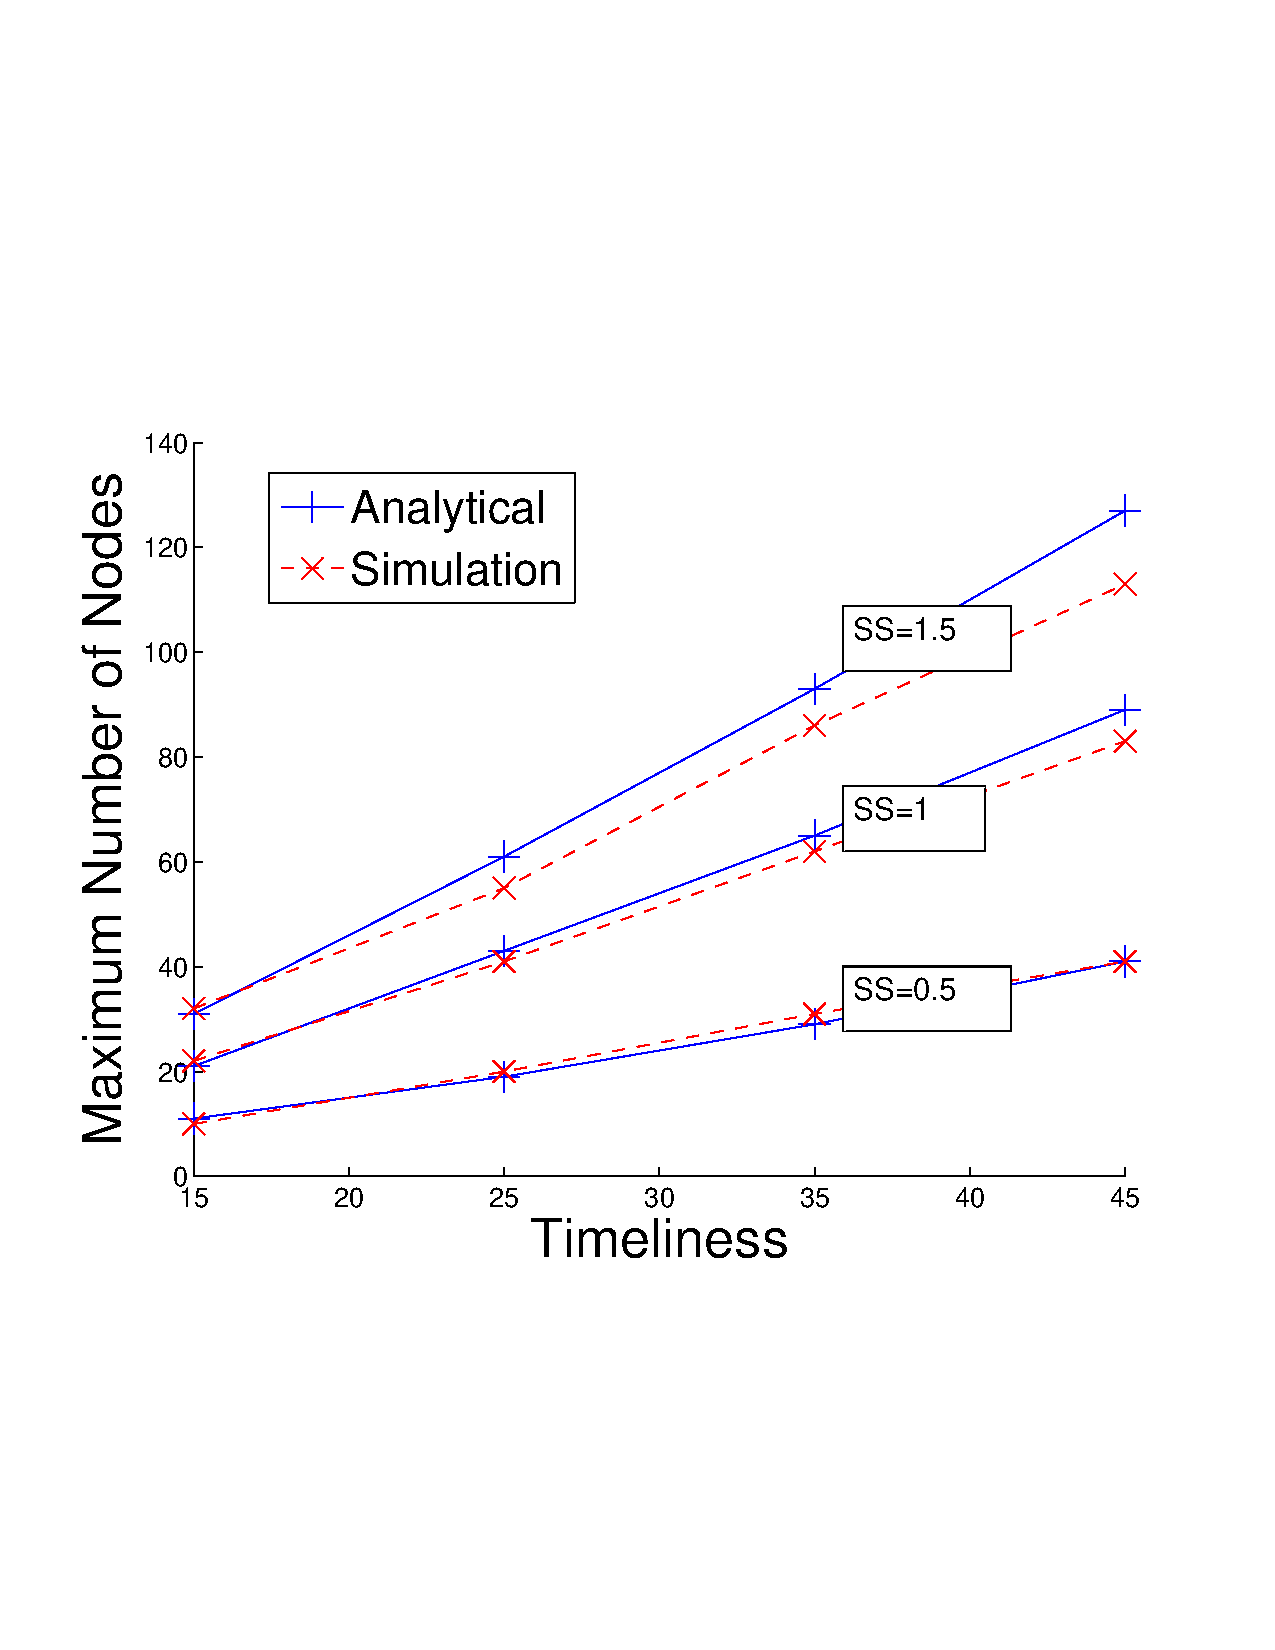
\includegraphics[scale=0.40, clip=true, trim=12mm 65mm 20mm 65mm]{figures/scal_sim_results/line_scal_anal_vs_sim_color.pdf}
%        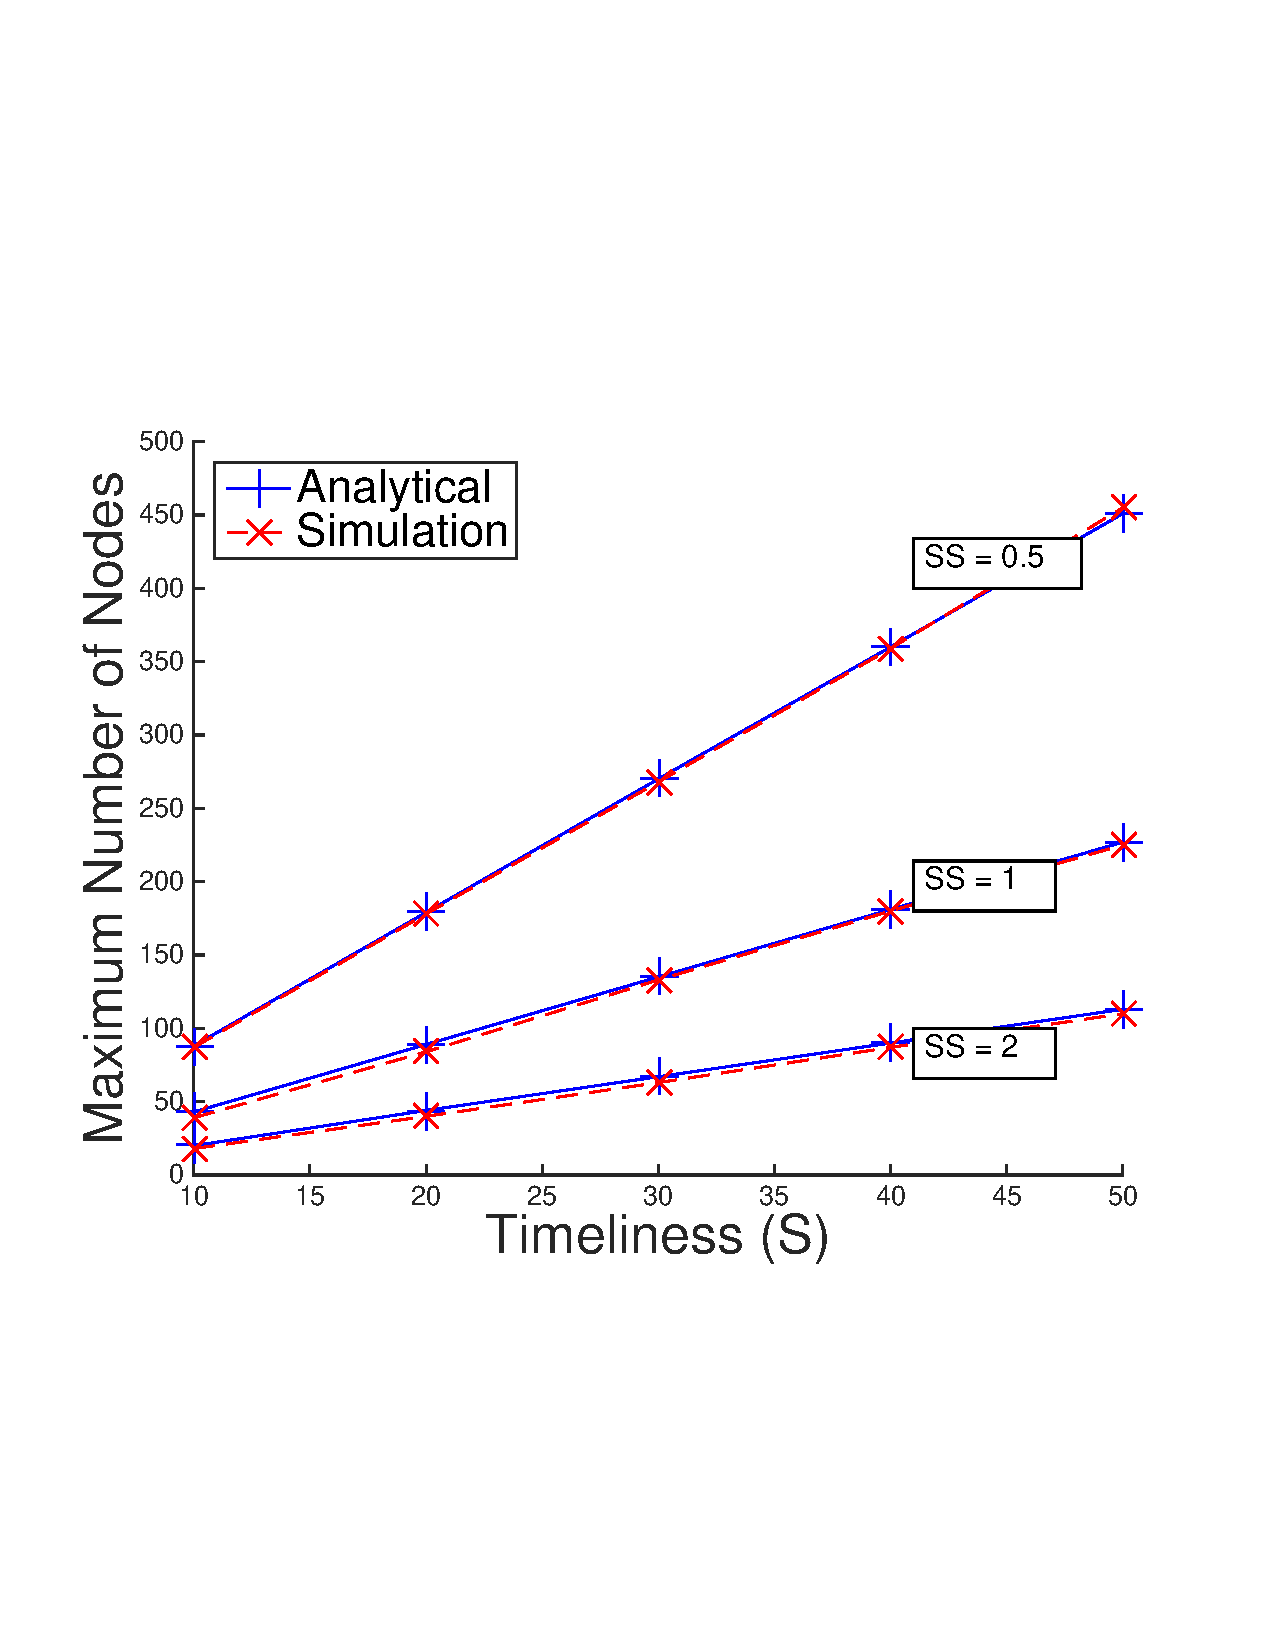
\includegraphics[scale=0.40, clip=true, trim=12mm 65mm 20mm 65mm]{figures/scal_sim_results/color_2d/line_uni_2d_qoi_vs_non_color_multiple.pdf}
        \label{fig:scal_vs_qoi_line}
        }
    \subfigure[Grid Network, $I_S = 48 KB$]{
%        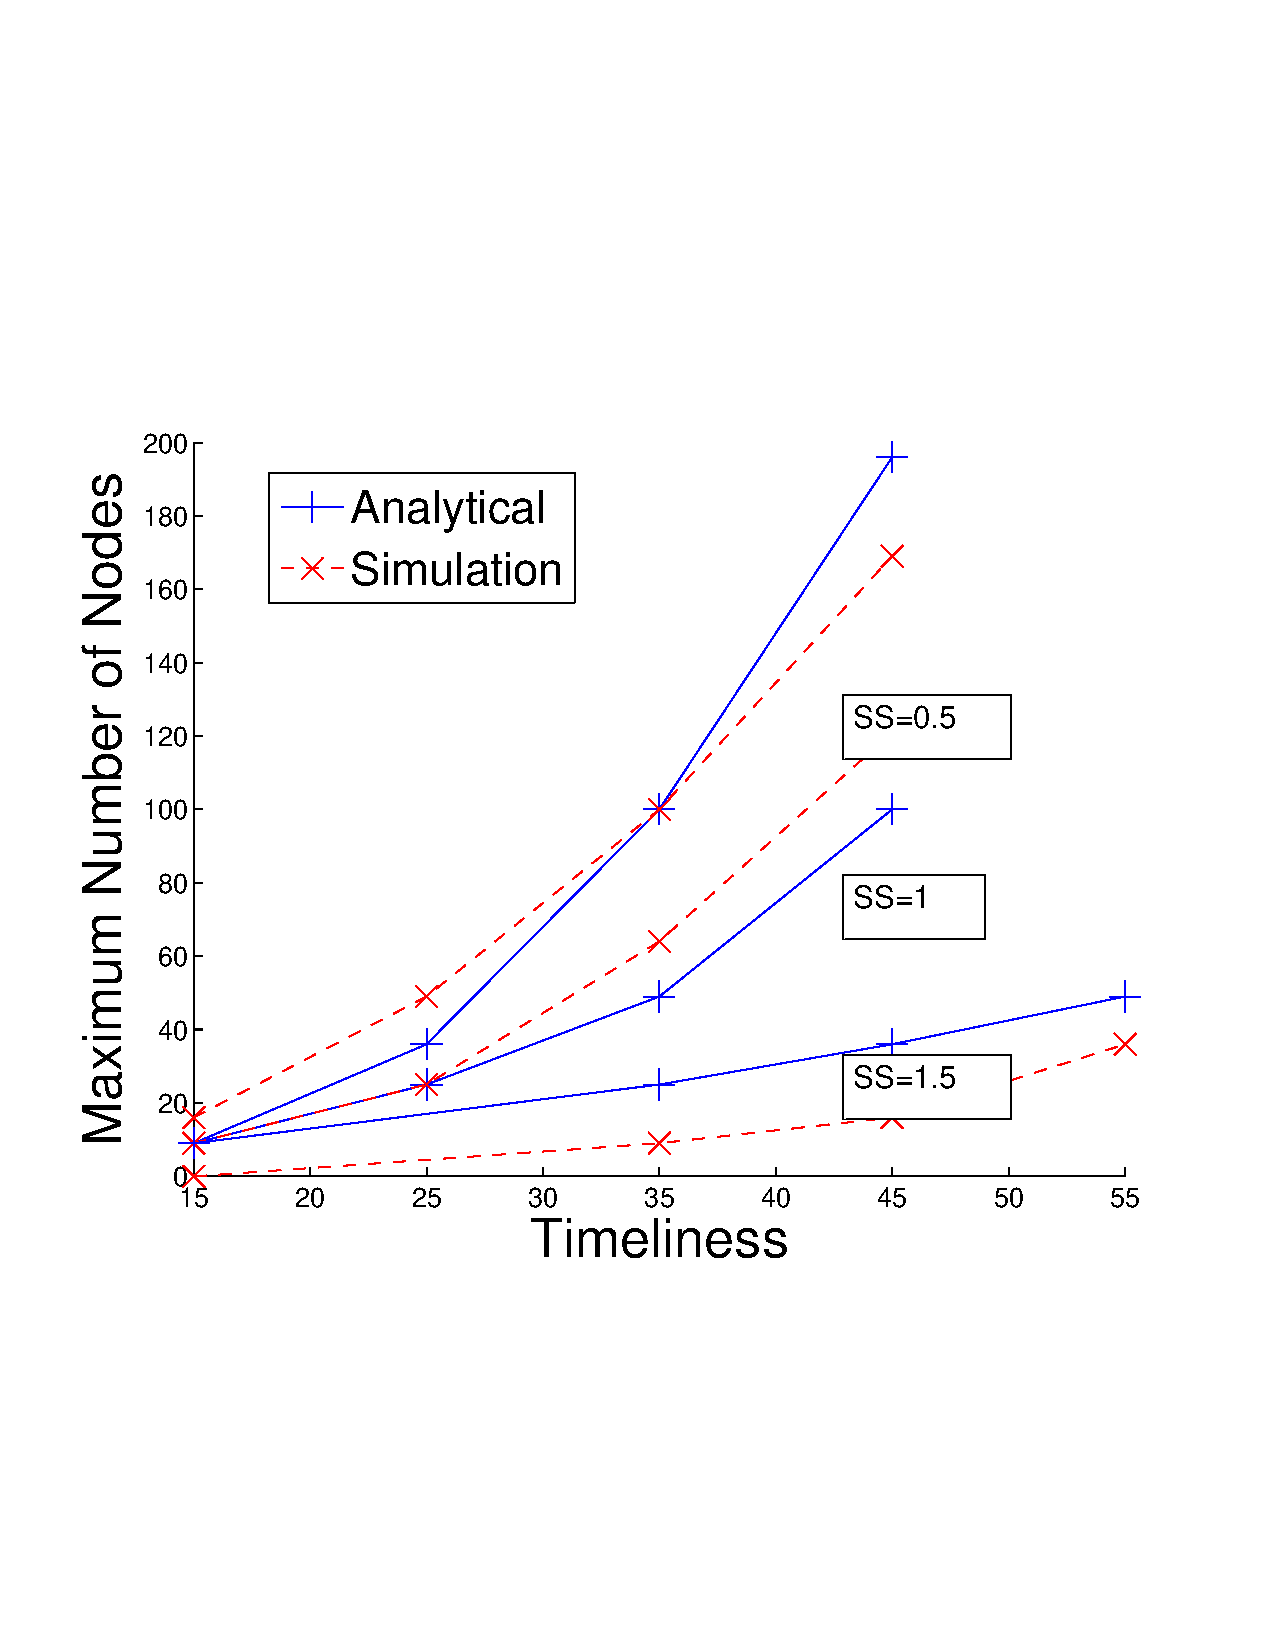
\includegraphics[scale=0.40, clip=true, trim=12mm 65mm 20mm 65mm]{figures/scal_sim_results/grid_scal_anal_vs_sim_color.pdf}
        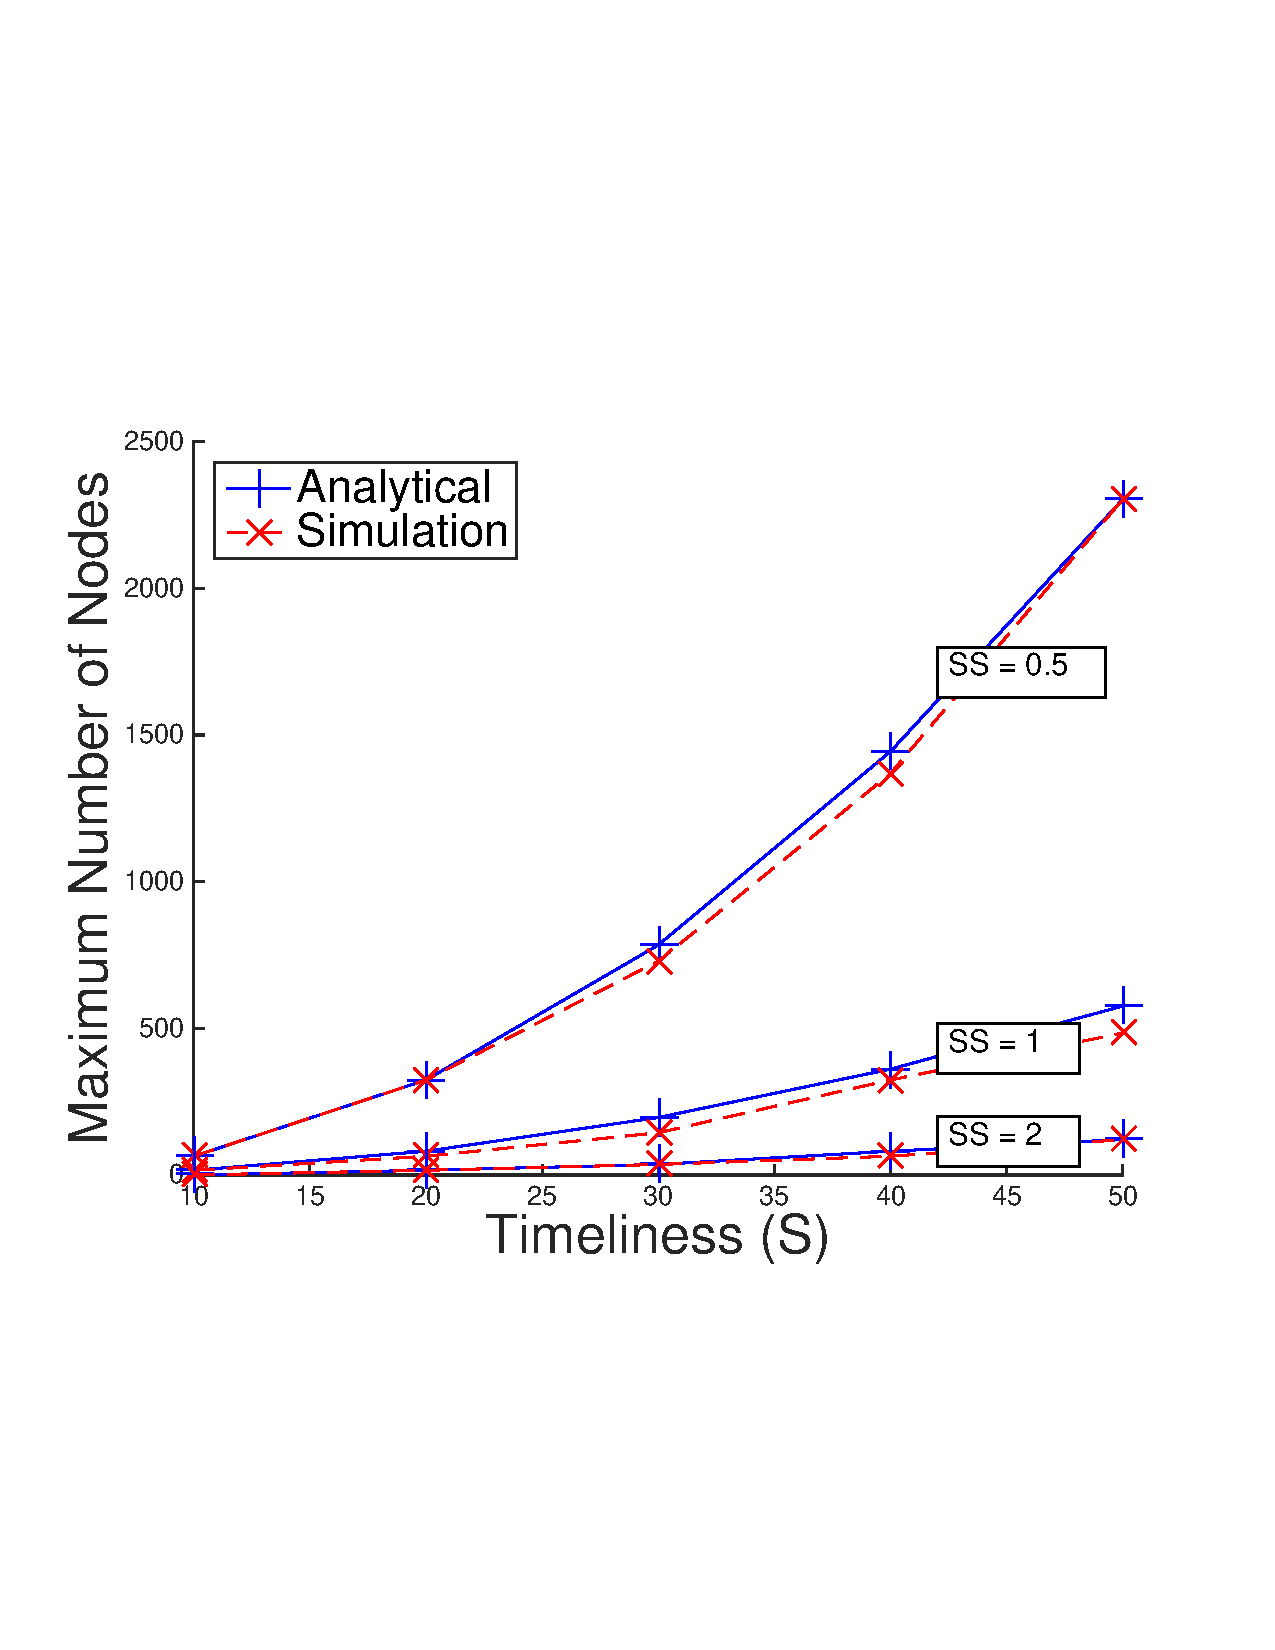
\includegraphics[scale=0.40, clip=true, trim=12mm 65mm 20mm 65mm]{figures/scal_sim_results/color_2d/grid_uni_2d_qoi_vs_non_color_multiple.pdf}
        \label{fig:scal_vs_qoi_grid}
        }
   \caption{Empirical results match analytical results closely for all tests.}
   \label{fig:scal_vs_qoi}
\end{figure}

To show how effective estimates using this framework can be, we simulated the network topologies and traffic described above in Section \ref{sec:example_applications} in the ns3 network simulator, comparing empirical results to those generated analytically with this framework, labeled \emph{Analytical}.  
%Due to space concerns, we only show a subset of results in Figure \ref{fig:scal_vs_qoi} to provide evidence of the effectiveness of the methodology.  All results generated, however, exhibit very similar trends of proximity between empirical and the analytical values.
We use a channel rate of $W= 2 Mbps$, packet sizes of $P_s = 1500$ bytes, and image sizes of $18$ and $48$ Kbytes.  As above, the correlation between Sum Similarity and $k_{req}$ is taken from the actual observed relation in Figure \ref{fig:topkSumSim}.  All values of parameters ($SS$, $T$, $I_S$, etc.) were chosen to test a variety of network sizes and QoI requirements while remaining within realistic network sizes, both with respect to real-world deployments and simulations with feasible run-times.



\section{Validation}
\label{sec:validation}

\begin{figure}[]
\centering
       \subfigure[Line Network, $I_S = 18 KB$]{
        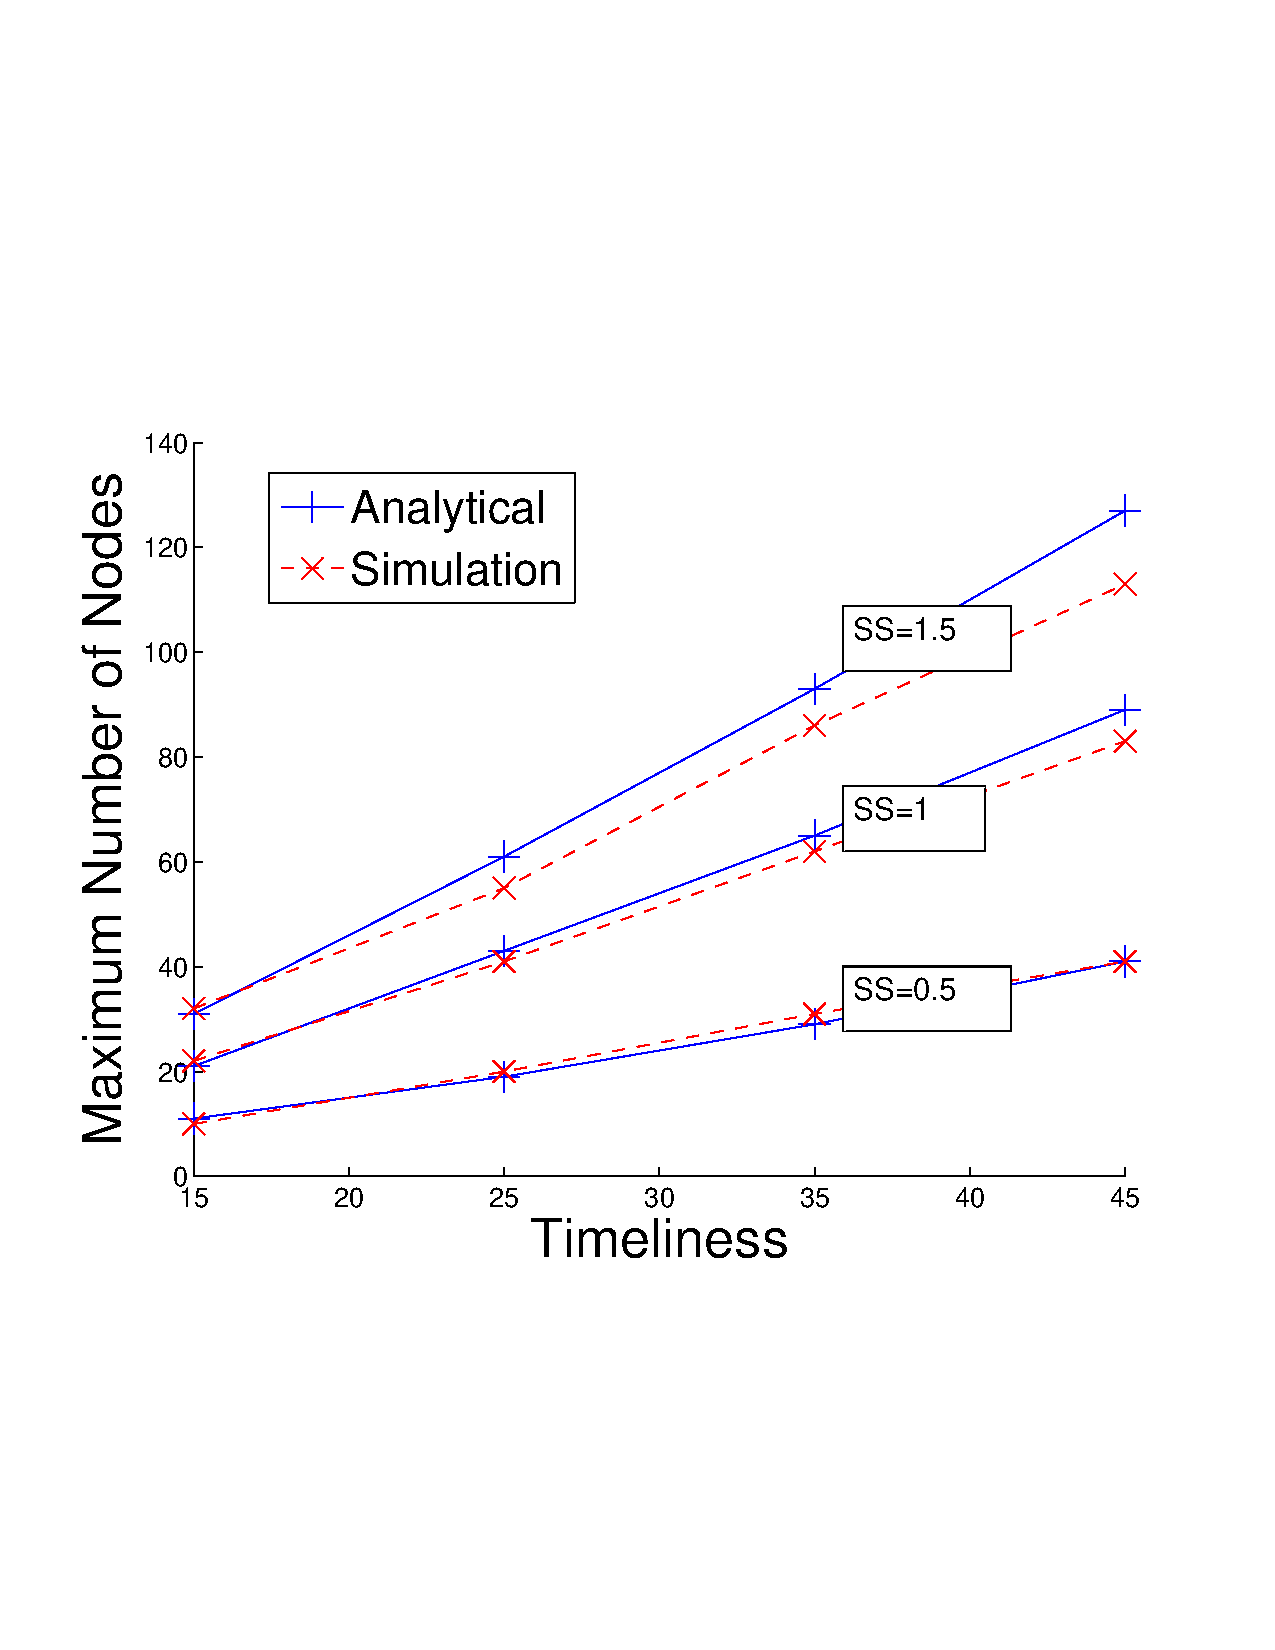
\includegraphics[scale=0.40, clip=true, trim=12mm 65mm 20mm 65mm]{figures/scal_sim_results/line_scal_anal_vs_sim_color.pdf}
        \label{fig:scal_vs_qoi_line}
        }
    \subfigure[Grid Network, $I_S = 48 KB$]{
        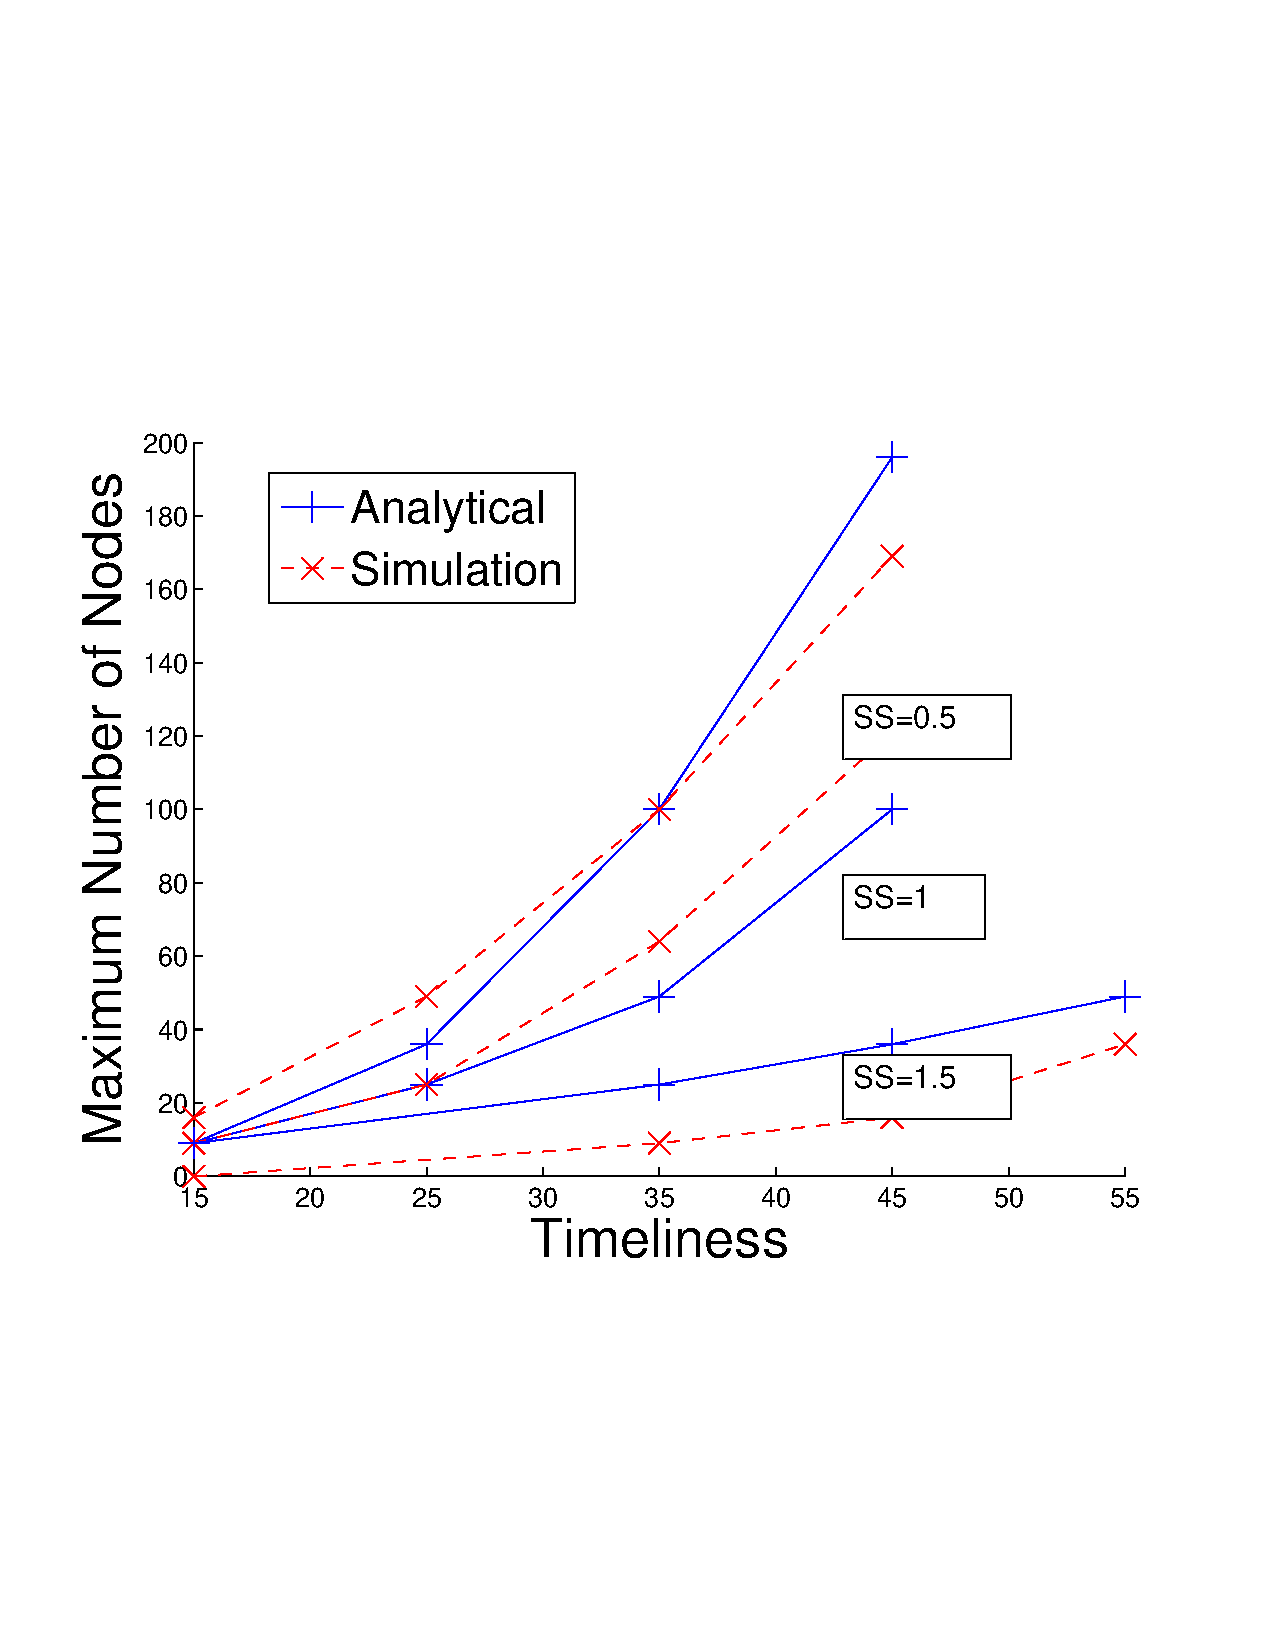
\includegraphics[scale=0.40, clip=true, trim=12mm 65mm 20mm 65mm]{figures/scal_sim_results/grid_scal_anal_vs_sim_color.pdf}
        \label{fig:scal_vs_qoi_grid}
        }
   \caption{Empirical results match analytical results closely for all tests.}
   \label{fig:scal_vs_qoi}
\end{figure}

To show how effective estimates using this framework can be, we simulated the network topologies and traffic described above in Section \ref{sec:example_applications} in the ns3 network simulator, comparing empirical results to those generated analytically with this framework, labeled \emph{Analytical}.  
%Due to space concerns, we only show a subset of results in Figure \ref{fig:scal_vs_qoi} to provide evidence of the effectiveness of the methodology.  All results generated, however, exhibit very similar trends of proximity between empirical and the analytical values.
We use a channel rate of $W= 2 Mbps$, packet sizes of $P_s = 1500$ bytes, and image sizes of $36$ and $72$ Kbytes.  As above, the correlation between Sum Similarity and $k_{req}$ is taken from the actual observed relation in Figure \ref{fig:topkSumSim}.  All values of parameters ($SS$, $T$, $I_S$, etc.) were chosen to test a variety of network sizes and QoI requirements while remaining within realistic network sizes, both with respect to real-world deployments and simulations with feasible run-times.

%Figure \ref{fig:scal_vs_qoi} shows the maximum scalability projected by solving inequalities (\ref{eq:clique_gen})-(\ref{eq:grid_gen}) and the maximum scalability observed in our experiments.  In our simulations, we defined \emph{scalable} as a network in which all of the requested queries were entirely fulfilled within the specified timeliness requirement.  Small differences arise due to average values being used for $CF$, $TF$, $DF$, and $PL$, but, as the graphs show, in all of these scenarios, our network size estimates are very close to those realized in practical simulations.


%\begin{figure*}[]
%\centering
%    \subfigure[Clique Network, $I_S = 9 MB$]{
%        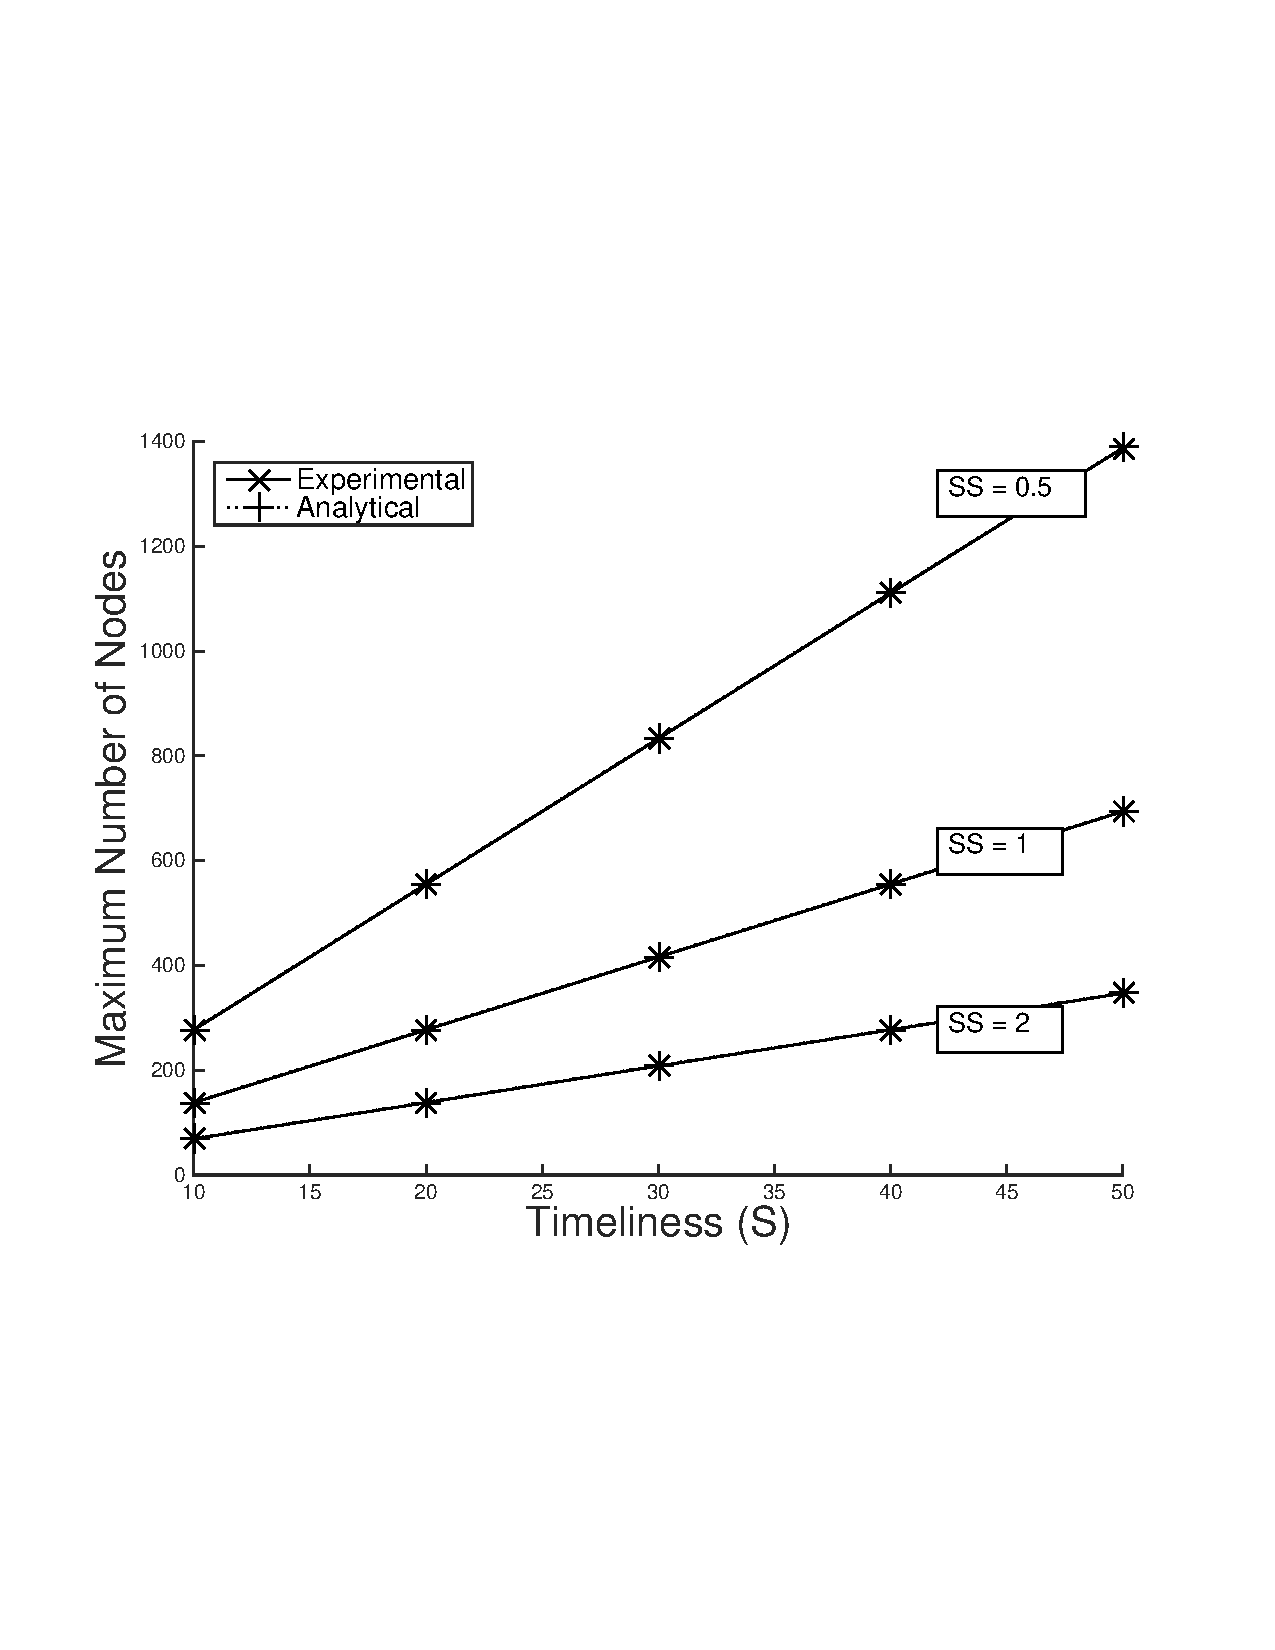
\includegraphics[scale=0.29, clip=true, trim=15mm 65mm 20mm 65mm]{figures/scal_sim_results/clique_uni_2d.pdf}
%        \label{fig:scal_vs_qoi_clique}
%        }
%    \subfigure[Line Network, $I_S = 12 MB$]{
%        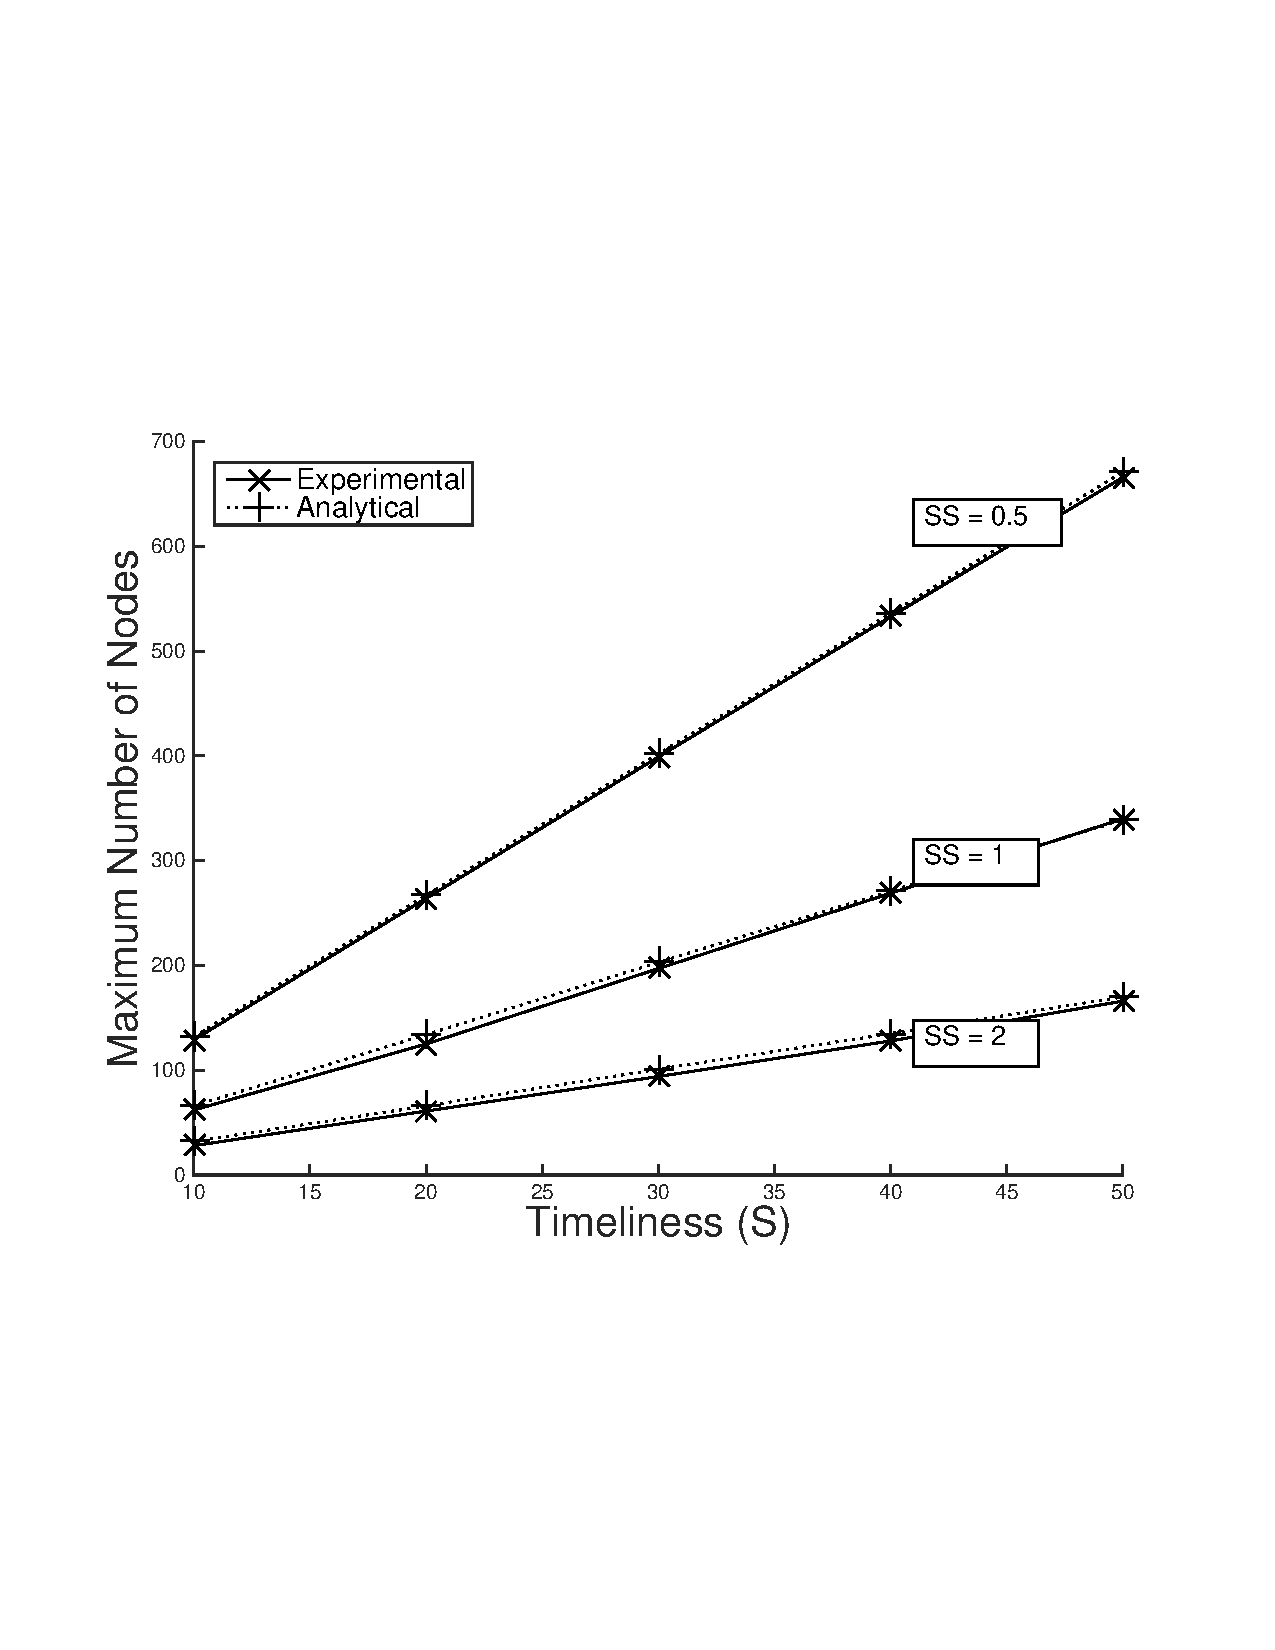
\includegraphics[scale=0.29, clip=true, trim=15mm 65mm 20mm 65mm]{figures/scal_sim_results/line_uni_2d_mhop_2.pdf}
%        \label{fig:scal_vs_qoi_line}
%        }
%    \subfigure[Grid Network, $I_S = 48 MB$]{
%        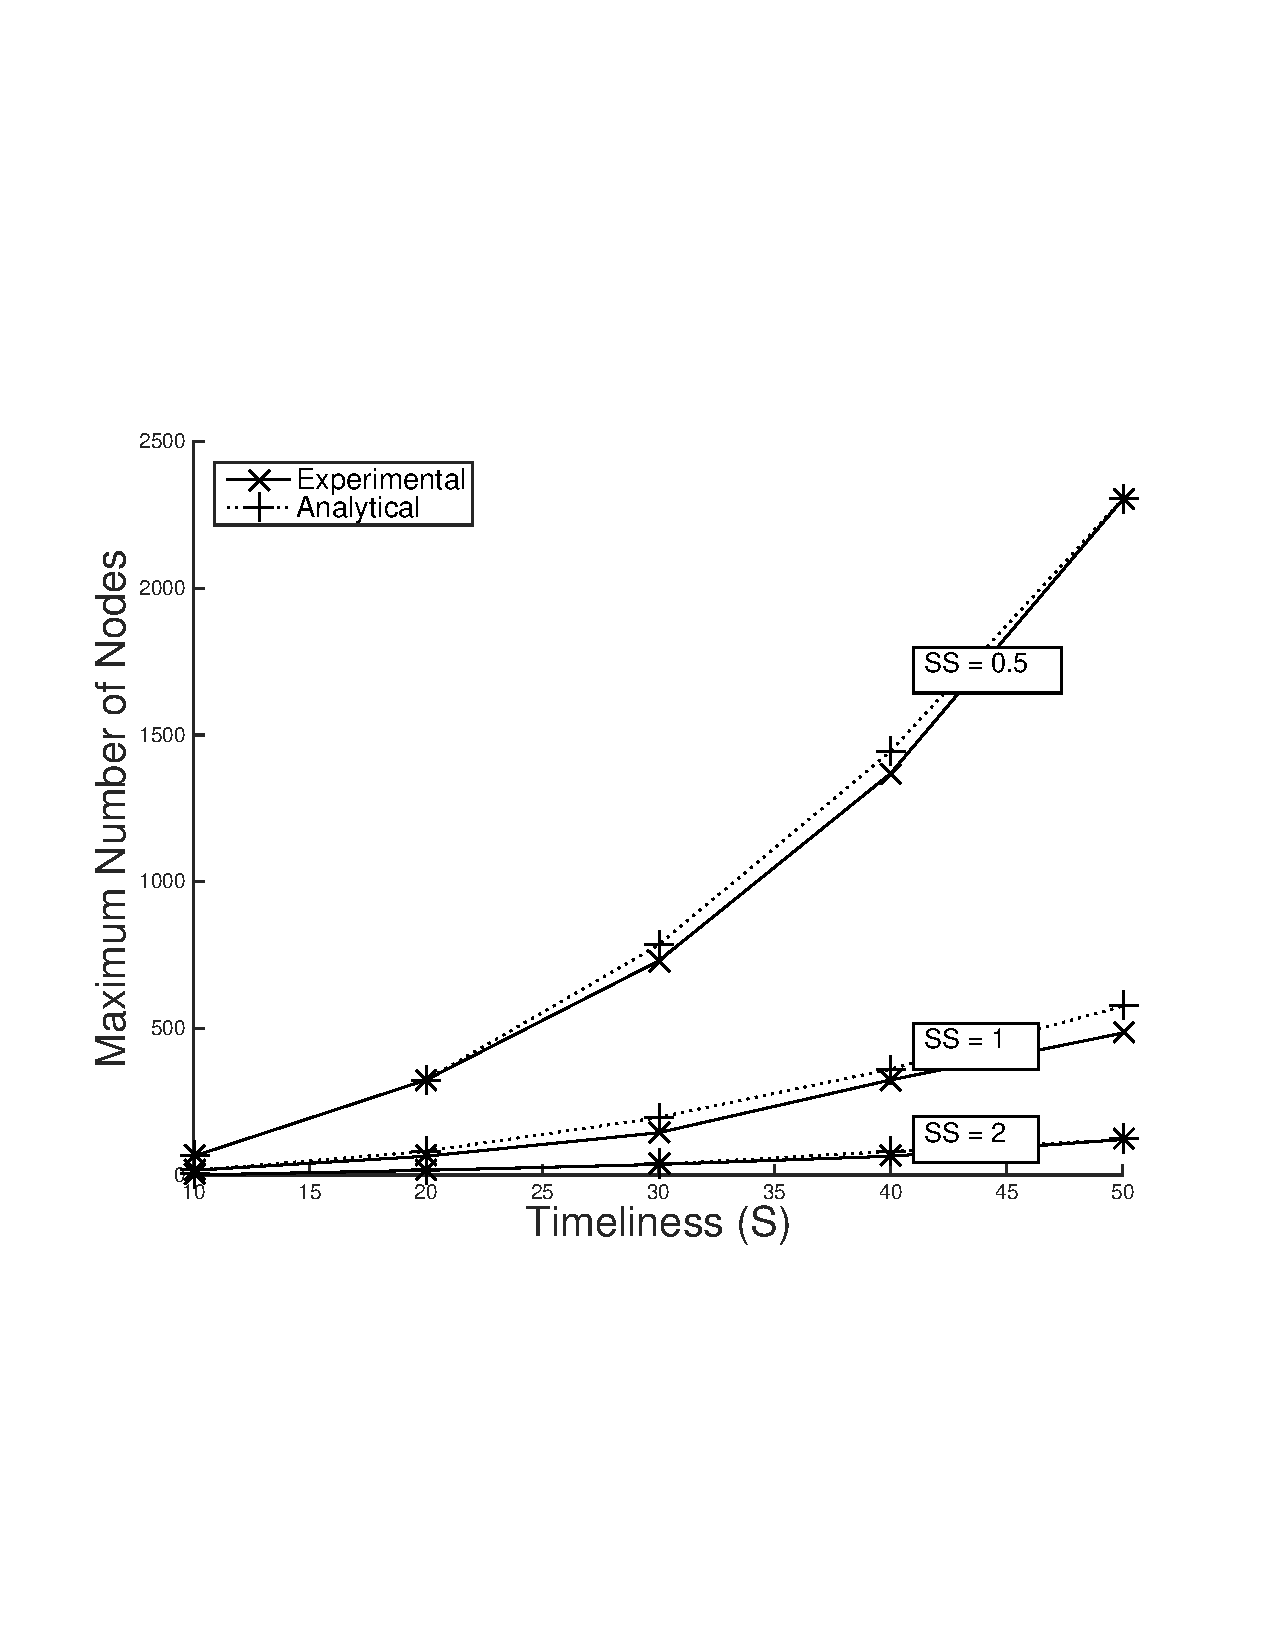
\includegraphics[scale=0.29, clip=true, trim=15mm 65mm 20mm 65mm]{figures/scal_sim_results/grid_uni_2d_mhop_2.pdf}
%        \label{fig:scal_vs_qoi_grid}
%        }
%   \caption{Empirical results match analytical results closely for all performed tests.  Results for each topology and a variety of sum similarity (SS) and timeliness requirements are provided.}
%   \label{fig:scal_vs_qoi}
%\vspace{-6mm}
%\end{figure*}


\section{Finding Limits and Characterizing Delay}
\label{sec:delay_char}
As explained in Section \ref{sec:qoi_model}, delay of a flow can be expressed as
\begin{equation}
	D = \frac{ k_{req} \cdot I_S \cdot CF \cdot TF}{W} + \frac{P_S \cdot DF \cdot (PL-1)}{W}
\end{equation}
%We will make some substitutions to get the following version
%\begin{equation}
%	D = \frac{ P_S \cdot CF \cdot P_N \cdot TF}{W} + \frac{P_S \cdot DF \cdot (PL-1)}{W}
%\end{equation}
%
Let $PL()$ be a function that provides the path length between $i$ and $j$, and let $TF_{i}^{j}$ be a random variable of the Traffic Factor for the bottleneck node between $i$ and $j$, i.e. the node along the path from $i$ to $j$ with the highest $u_x$.  Finally, let $P_N$ be a random variable that describes the number of packets in a given request, capturing both the possible randomness of $k_{req}$ and $I_S$.  
Then, building on the equation for delay above and making some substitutions, we can get the following equation to describe the delay from a node $i$ given a destination of $j$:
\begin{equation}
	D_{i}^{j} = \frac{ P_S \cdot CF \cdot P_N \cdot TF_{i}^{j}}{W}  + \frac{P_S \cdot DF \cdot (PL(i,j)-1)}{W}
\end{equation}

%Also, recall that $TF$ is a random variable of the flows being forwarded at the bottleneck node along the path of the flow.  
Defining two constants to simplify the expression,
\begin{eqnarray*}
	C_1 = \frac{P_S \cdot CF}{W} \\
	C_2 = \frac{P_S \cdot DF}{W}
\end{eqnarray*}
we can express the delay as
\begin{equation}
	D_{i}^{j} = C_1 \cdot P_N \cdot TF_{i}^{j} + C_2 \cdot PL(i,j)
\end{equation}

We can develop an expression for a distribution of delay as follows.  First, we define the cumulative distribution of a source-destination pair $(i,j)$:
\begin{equation*}
	P( D_{i}^{j} \leq d ) = P( C_1 \cdot P_N \cdot TF_{i}^{j} + C_2 \cdot PL(i,j) \leq d )
\end{equation*}
\begin{equation*}
	= P( P_N \cdot TF_{i}^{j} \leq \frac{d - C_2 \cdot PL(i,j)}{C_1}  )
\end{equation*}
Next, conditioning over all possible values of $TF$, we get
\begin{equation*}
	P( D_{i}^{j} \leq d ) = \sum\limits_{\tau = 1}^{\tau_{max}} P( P_N \cdot TF \leq \frac{d - C_2 \cdot PL(i,j)}{C_1} | TF = \tau ) \cdot f_{TF_{i}^{j}}(\tau)
\end{equation*}
\begin{equation*}
	= \sum\limits_{\tau = 1}^{\tau_{max}} P( P_N \leq \frac{d - C_2 \cdot PL(i,j)}{C_1 \cdot \tau} ) \cdot f_{TF_{i}^{j}}(\tau)
\end{equation*}
Substituting the cumulative distribution representing the data load, $F_{P_{N}}$:
\begin{equation*}
	F_{D_{i}^{j}}(d) = \sum\limits_{\tau = 1}^{\tau_{max}} F_{P_N}( \frac{d - C_2 \cdot PL(i,j)}{C_1 \cdot \tau} ) \cdot f_{TF_{i}^{j}}(\tau)
\end{equation*}
Then, we can generalize the expression to give a distribution for a flow originating in node $i$ with an unknown destination by conditioning over all possible destinations, $j$.
\begin{equation}
\label{eq:delay_dist_pdf_i}
	F_{D_i} = \sum\limits_{j \neq i} [ \sum\limits_{\tau = 1}^{\tau_{max}} F_{P_N}( \frac{d - C_2 \cdot PL(i,j)}{C_1 \cdot \tau} ) \cdot f_{TF_{i}^{j}}(\tau) ] \cdot p(j)
\end{equation}
Finally, we can get an average distribution of all flows' delays by summing over all sources and dividing by the the number of sources.  This average delay distribution is in Equation (\ref{eq:full_delay_cdf}).

%\begin{figure*}[!t]
%\begin{equation}
%\label{eq:full_delay_cdf}
%	F_D(d) = \frac{1}{N} \cdot \sum\limits_{i = 1}^N \sum\limits_{j \neq i} \sum\limits_{tf=1}^{tf_{max}}  F_{P_N}( \frac{d - C_2 \cdot PL(i,j)}{C_1 \cdot p_N} ) \cdot f_{TF_{i | j}}( tf ) \cdot p(j)
%\end{equation}
%\end{figure*}

\begin{figure}[]
\centering
       \subfigure[Line Network, $N = 40$, $I_S = 36 KB$]{
%        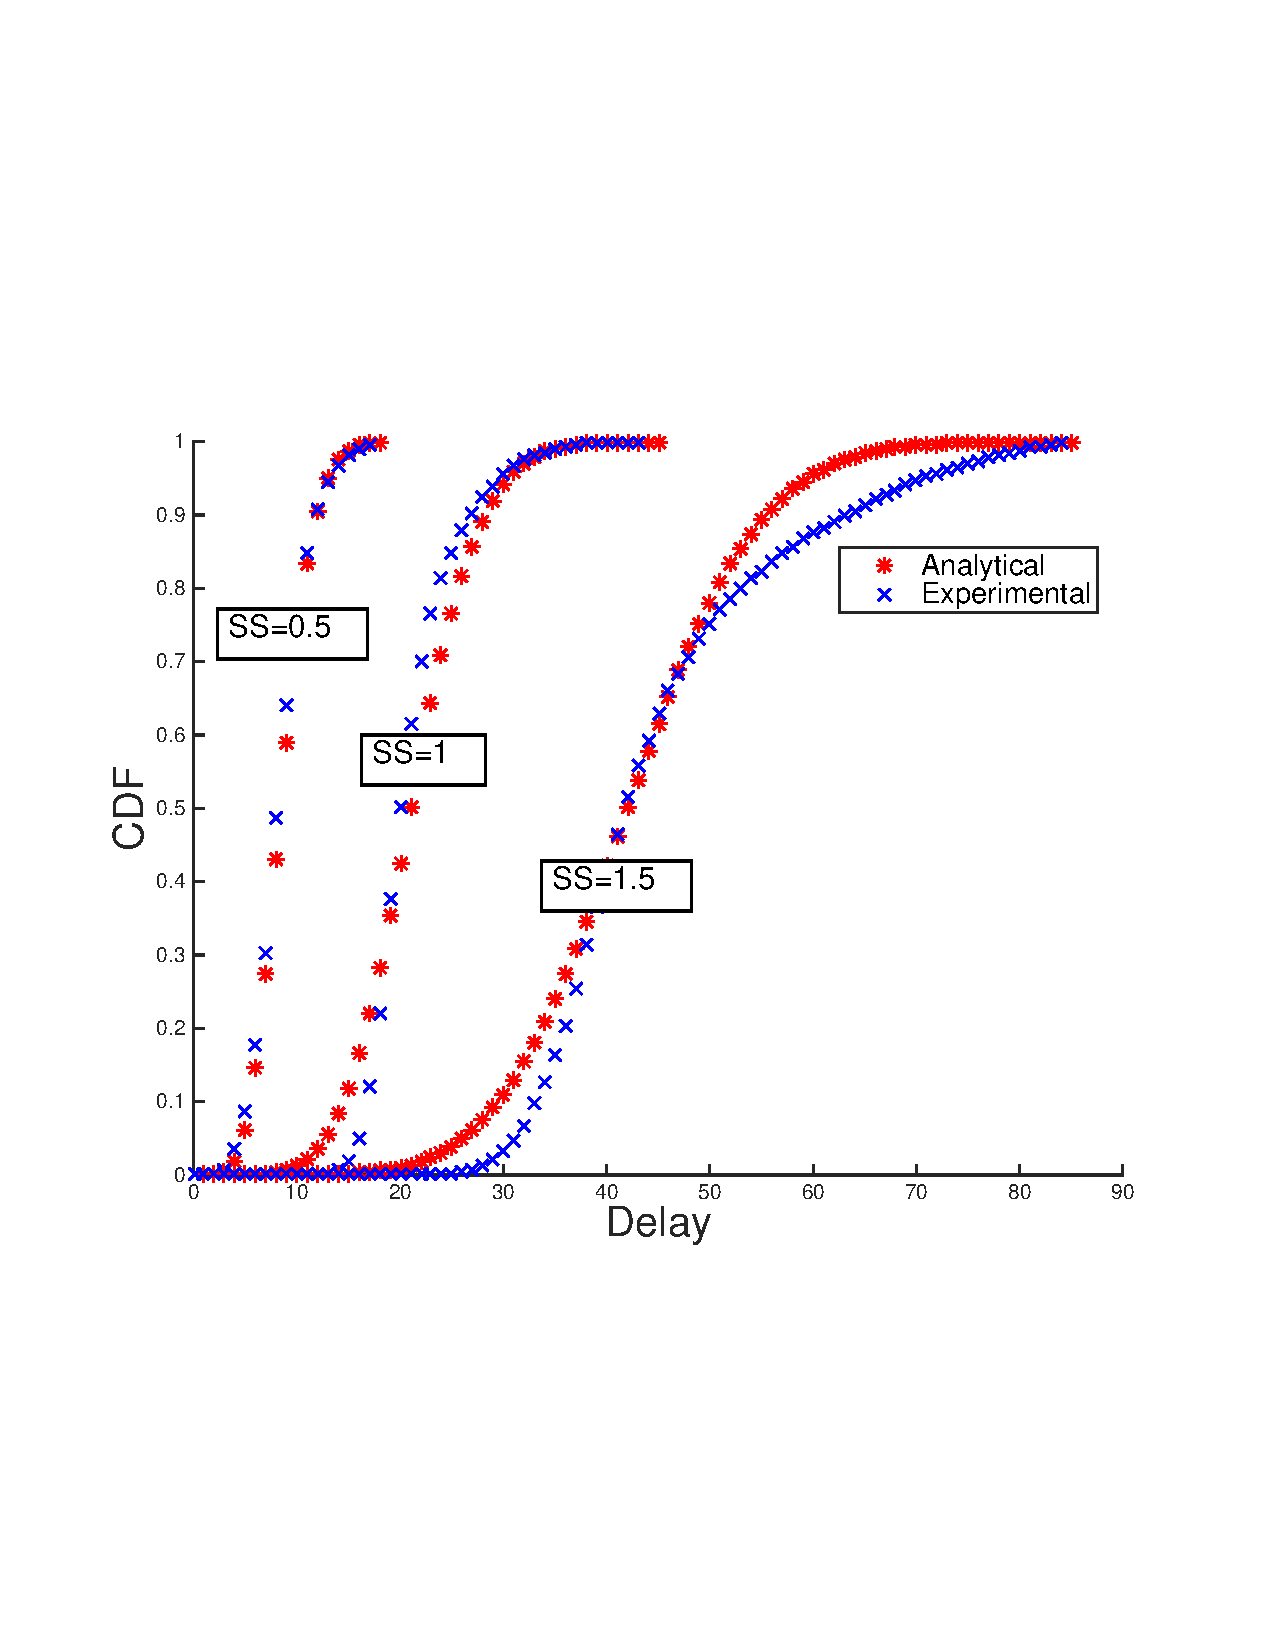
\includegraphics[scale=0.40, clip=true, trim=12mm 65mm 20mm 65mm]{figures/delay_cdfs/delay_cdf_line.pdf}
%        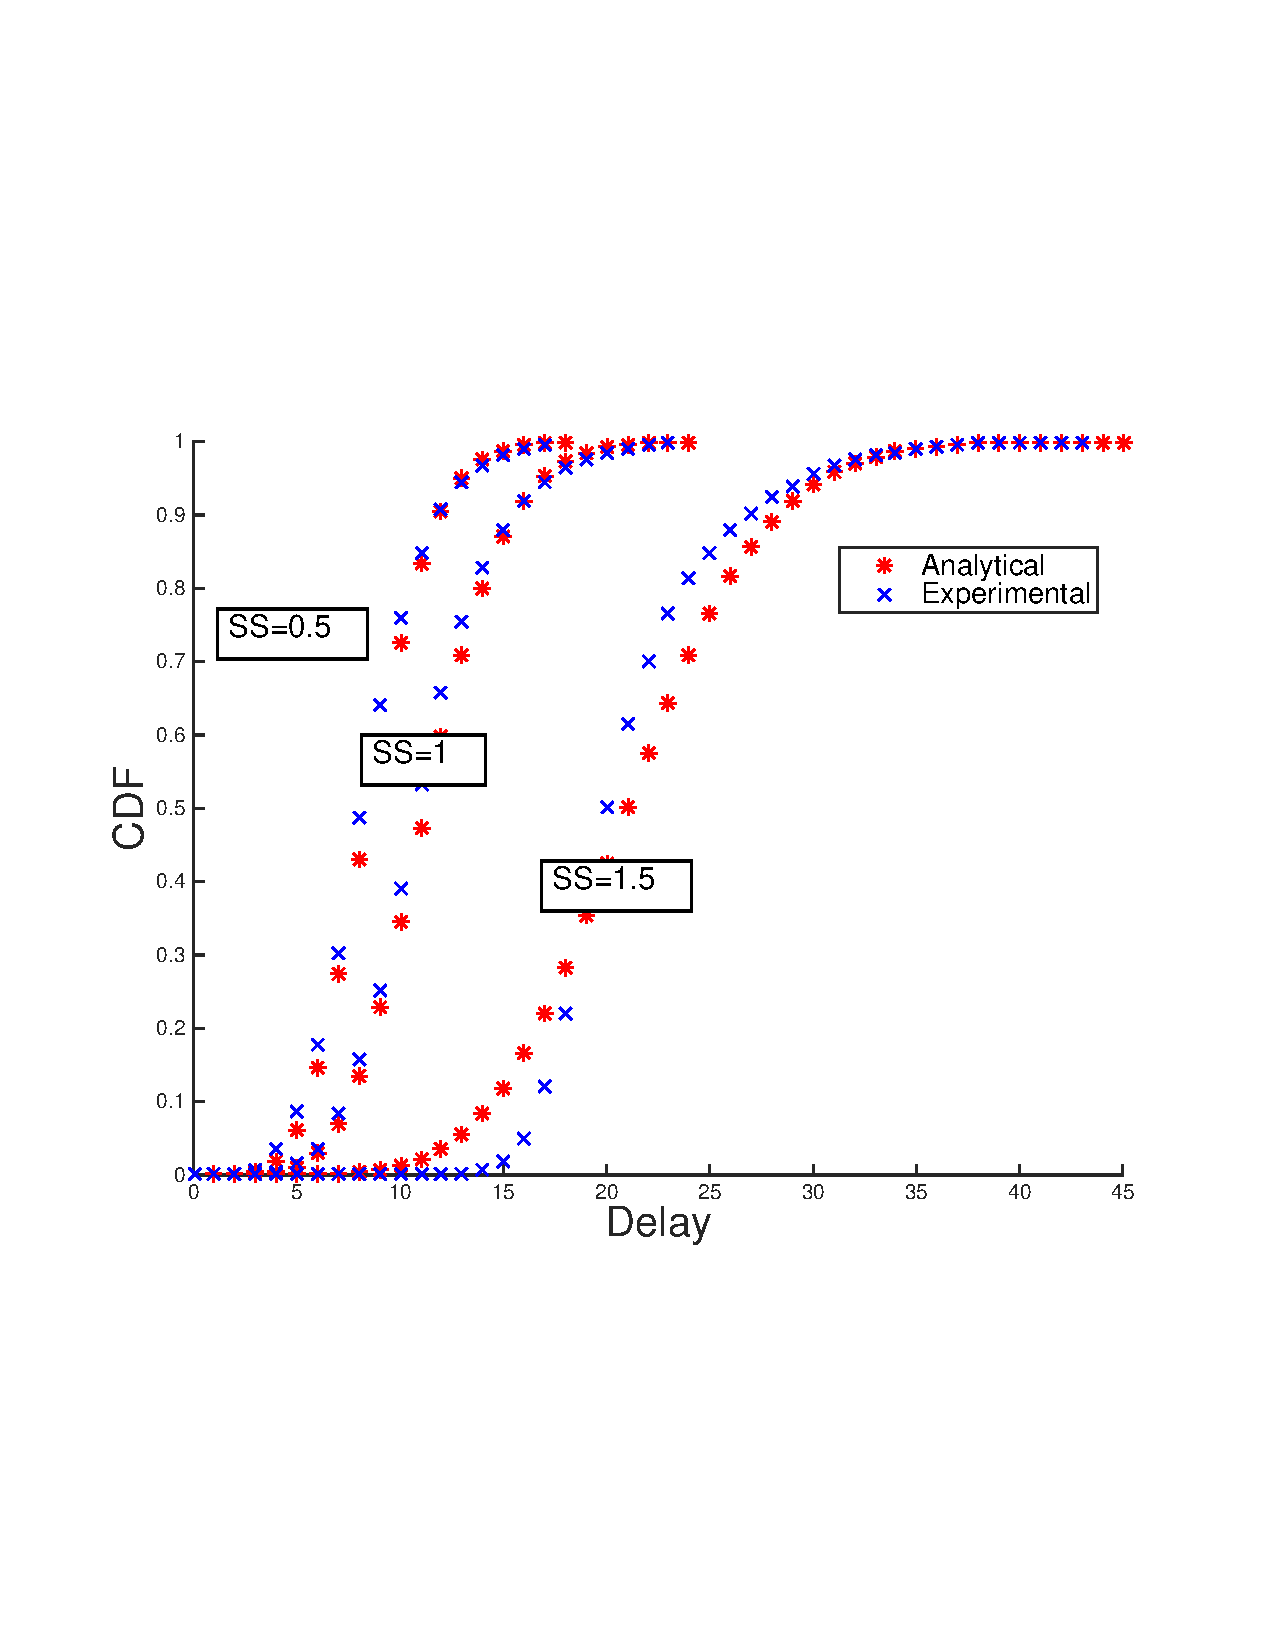
\includegraphics[scale=0.40, clip=true, trim=12mm 65mm 20mm 65mm]{figures/delay_cdfs/delay_cdf_line_full_2.pdf}
        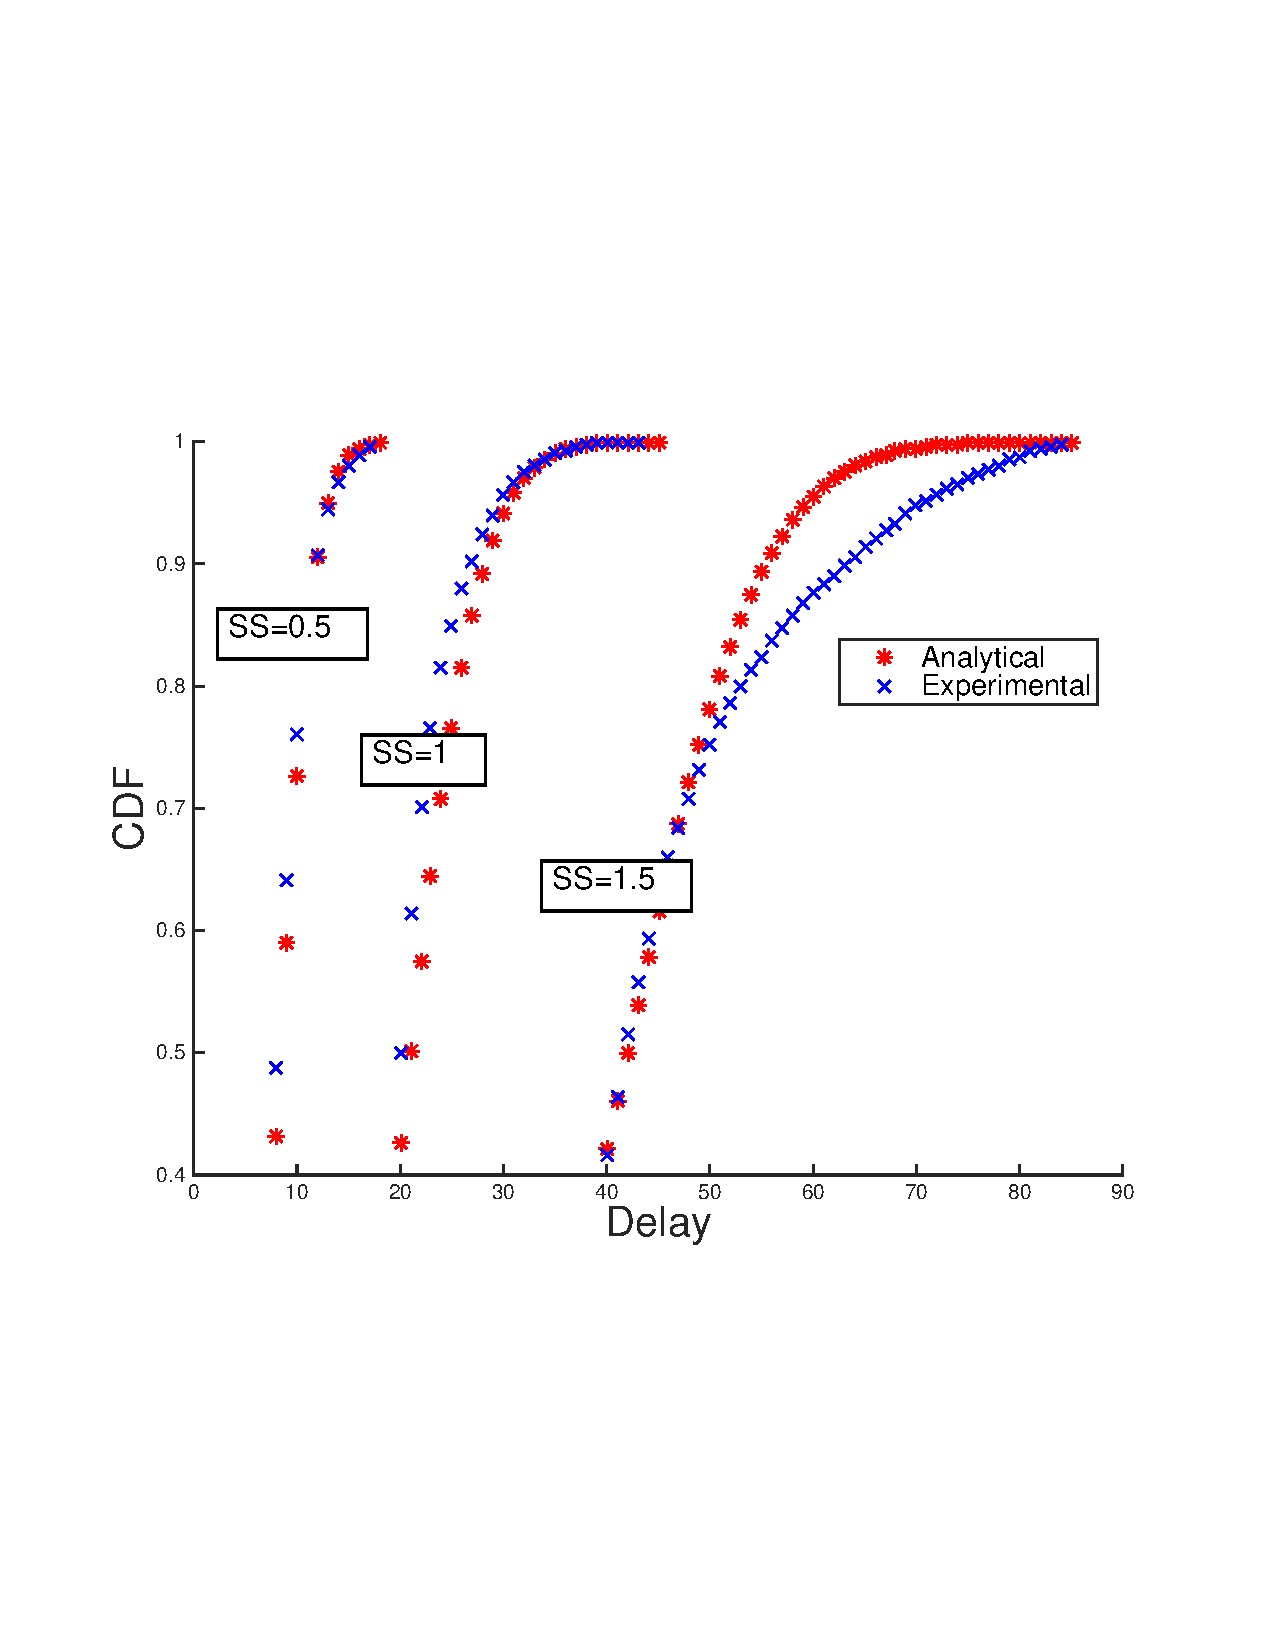
\includegraphics[scale=0.40, clip=true, trim=12mm 65mm 20mm 65mm]{figures/delay_cdfs/delay_cdf_line_half.pdf}
        \label{fig:scal_vs_qoi_line}
        }
    \subfigure[Grid Network, $N = 49$, $I_S = 72 KB$]{
%        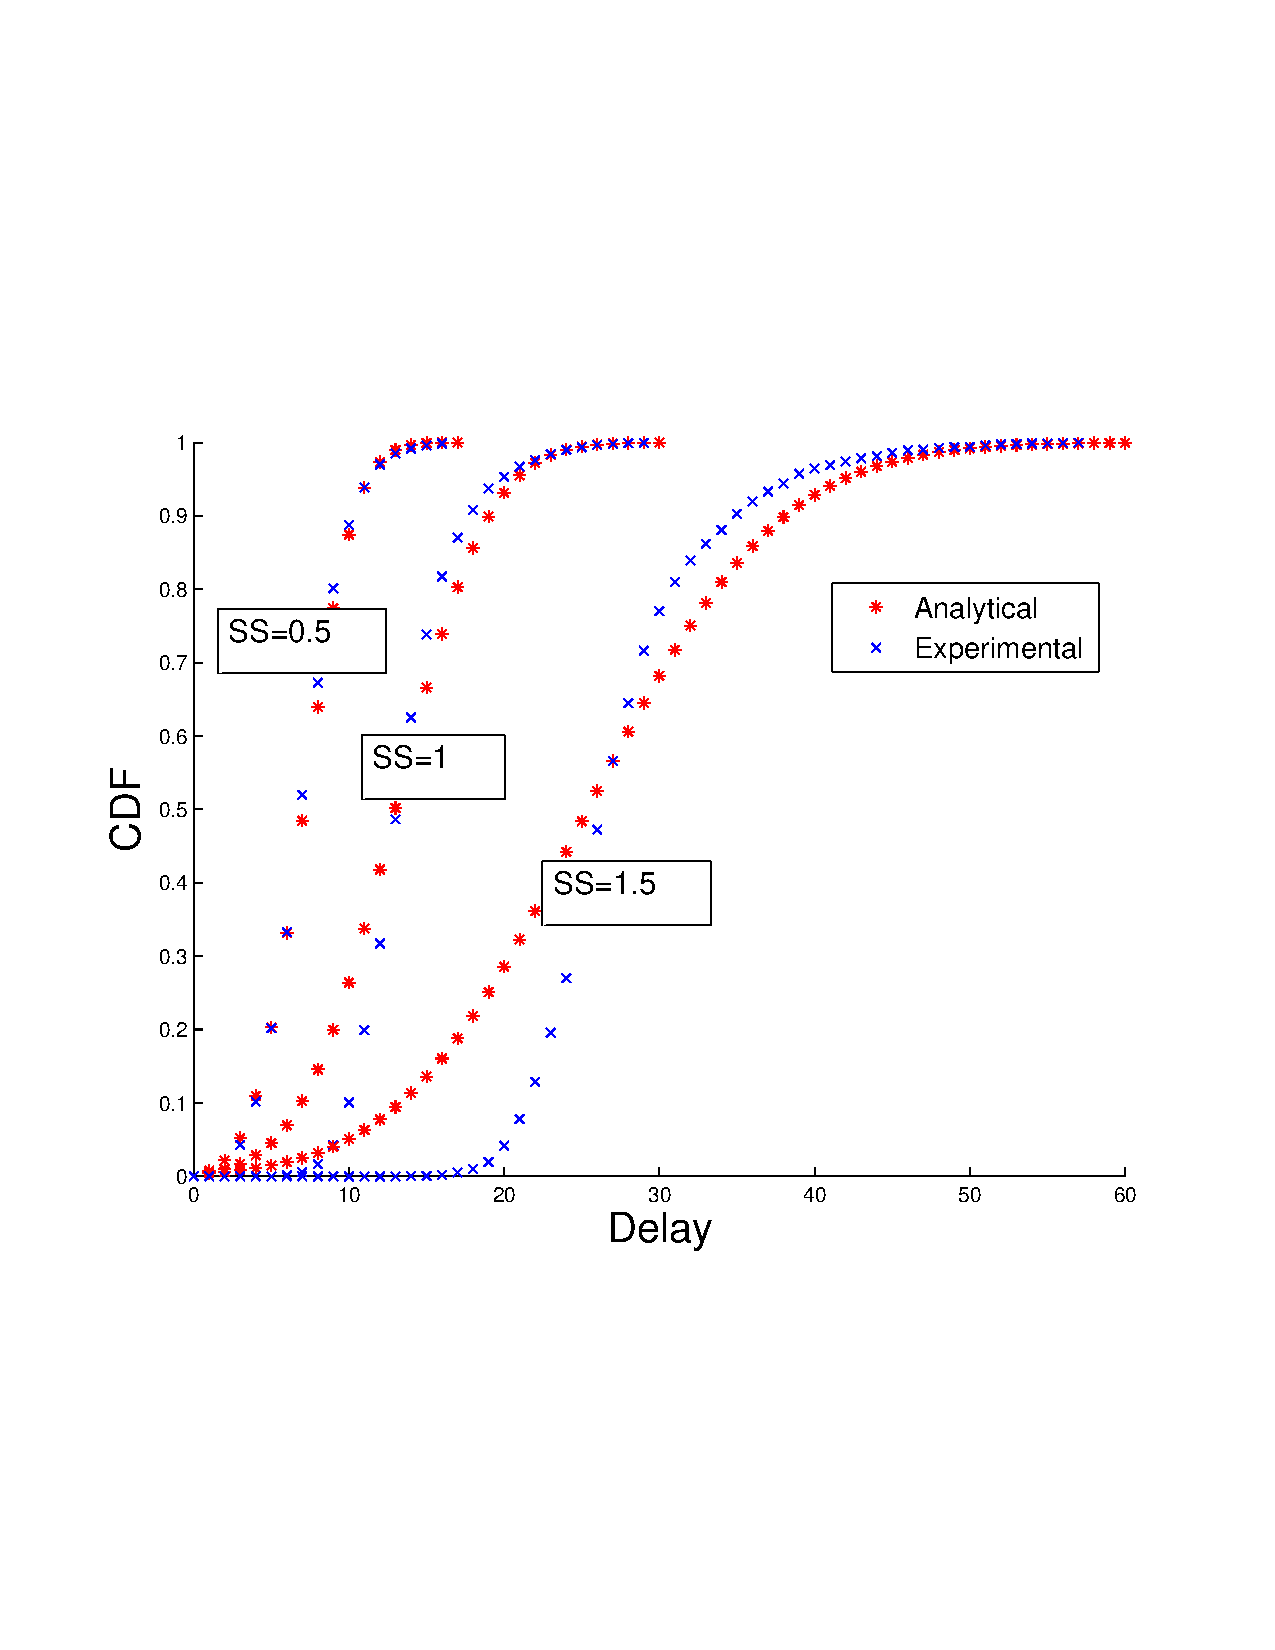
\includegraphics[scale=0.40, clip=true, trim=12mm 65mm 20mm 65mm]{figures/delay_cdfs/delay_cdf_grid.pdf}
        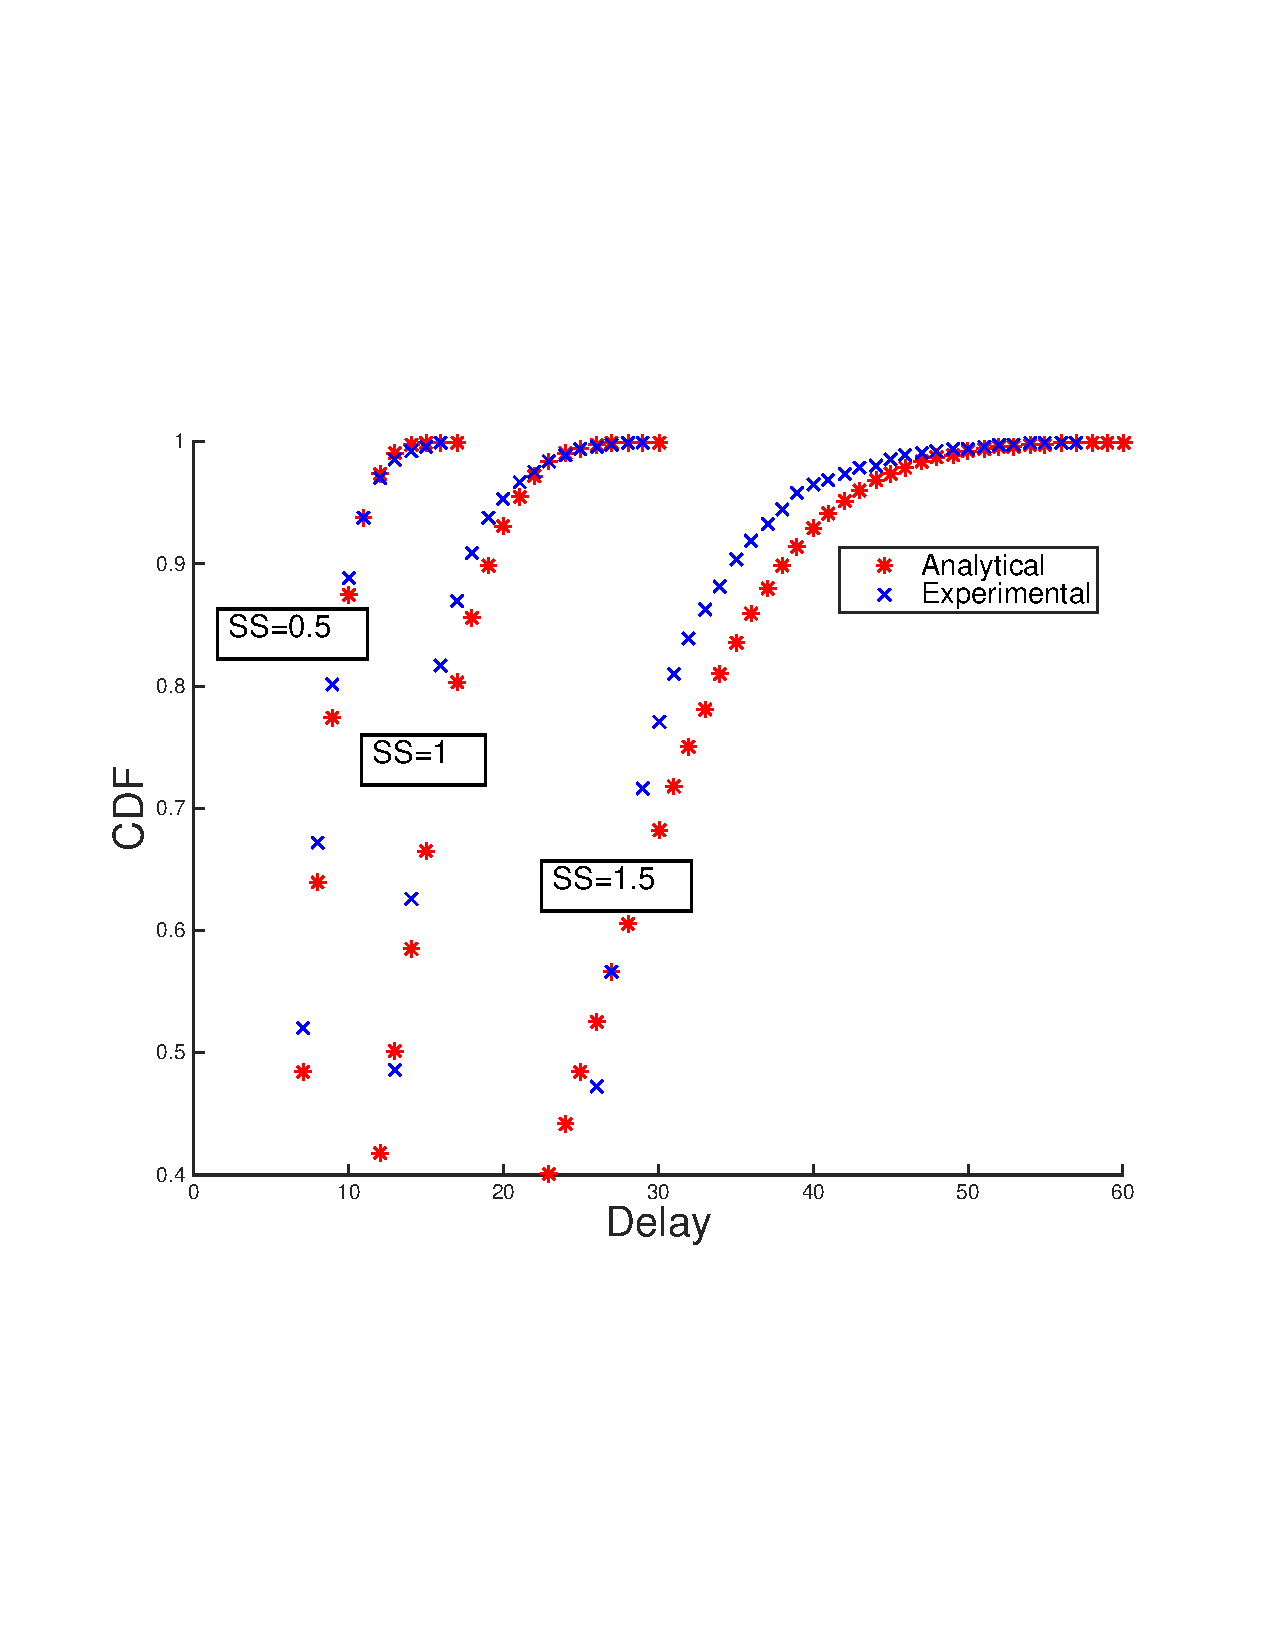
\includegraphics[scale=0.40, clip=true, trim=12mm 65mm 20mm 65mm]{figures/delay_cdfs/delay_cdf_grid_half.pdf}
        \label{fig:scal_vs_qoi_grid}
        }
   \caption{Characterization of delay using framework follows distribution of empirical results in most cases.}
   \label{fig:delay_cdf_anal_vs_sim}
\end{figure}

\subsection{Probability of Timeliness Satisfiability}

While the minimum timeliness at which all flows are expected to complete before their deadlines can be determined by the scalability equations in Section \ref{sec:example_applications}, some applications may benefit from an understanding of what the probability of completing within the timeliness constraints for those below the minimum fully satisfiable timeliness.  For example, if a mission issues a number of queries for information to support decision-making, receiving $80\%$ or $90\%$ of the responses may be sufficient for making the decision.  The question of importance, then, is "How far can we reduce the timeliness constraint and still expect to receive $x\%$ of the queries in time?"  Or, equivalently, we may pose the question, "When the network is operating at the edge of capacity, what is the expected delay for $x\%$ of queries to be completed?"  Since equation \ref{eq:full_delay_cdf} provides the distribution of delays, it provides quality estimates to answer these questions.  

\subsection{Validation of Delay Characterization}

Figure \ref{fig:delay_cdf_anal_vs_sim} shows expected delay distributions from \ref{eq:full_delay_cdf} alongside distributions of delays recorded in ns3 simulations of the same networks.  We argue that minimum QoI requirements for most applications tend to be over $50\%$, and therefore focus on the top half of the delay distribution.  In all cases here, analytical predictions of satisfying the timeliness requirement are within about $10\%$ of empirical results for probabilities above $0.5$.  

%Additionally, in smaller data load requirement cases, analytical predictions match simulation results quite closely along the entire distribution.

%\subsection{Scalability and Maximum QoI Equations}
%
%Once 

% from a different script:
%\subsubsection{Delay}
%
%The delay distribution for a flow beginning in source node $i$ is:
%
%\begin{equation}
%	f_{D_i} = \sum\limits_{j \neq i} [C_1 \cdot f_{TF_{i | j}}(tf) + C_2 \cdot PL(i,j)] \cdot p(j)
%\end{equation}
%which is equivalent to:
%\begin{equation}
%	P(D_i < d) = \sum\limits_{j \neq i} f_{TF_{i | j}}( \frac{d - C_2 \cdot PL(i,j)}{C_1} ) \cdot p(j)
%\end{equation}

%which can be expanded to:
%
%\begin{figure*}[t]
%\begin{eqnarray}
%\nonumber
%	f_{D_i} (d) = &&\frac{i}{N} \cdot \mathcal{N}( \frac{2(i-1)(N-i)}{(N-2)(N-1)} , \sqrt{\frac{2(i-1)(N-i)  (1-\frac{1}{N-1})}{(N-2)(N-1)}} )  \\ \nonumber
%			   &+& \sum\limits_{k=i}^{\frac{N}{2}-1} \cdot \frac{\frac{1}{2}-\frac{i}{N}}{\frac{N}{2} - i}\mathcal{N}( \frac{2(k-1)(N-k)}{(N-2)(N-1)}, \sqrt{\frac{2(k-1)(N-k)}{(N-2)(N-1)} (1-\frac{1}{N-1})} )  \\
%			   &+& \frac{1}{2} \cdot \mathcal{N} ( \frac{N(\frac{N}{2}-1)}{(N-2)(N-1)} , \sqrt{\frac{N(\frac{N}{2}-1)}{(N-2)(N-1)} (1-\frac{1}{N-1})} )
%\label{eq:full_PDF_TF_line_2}
%\end{eqnarray}
%\end{figure*}
% end from different script


\section{Impact on Network Design}
\label{sec:network_design}

\begin{figure*}
\vspace{2mm}
\centering
    \subfigure[Max Timeliness vs. Network Size (Sum Sim. = 5.0)]{
	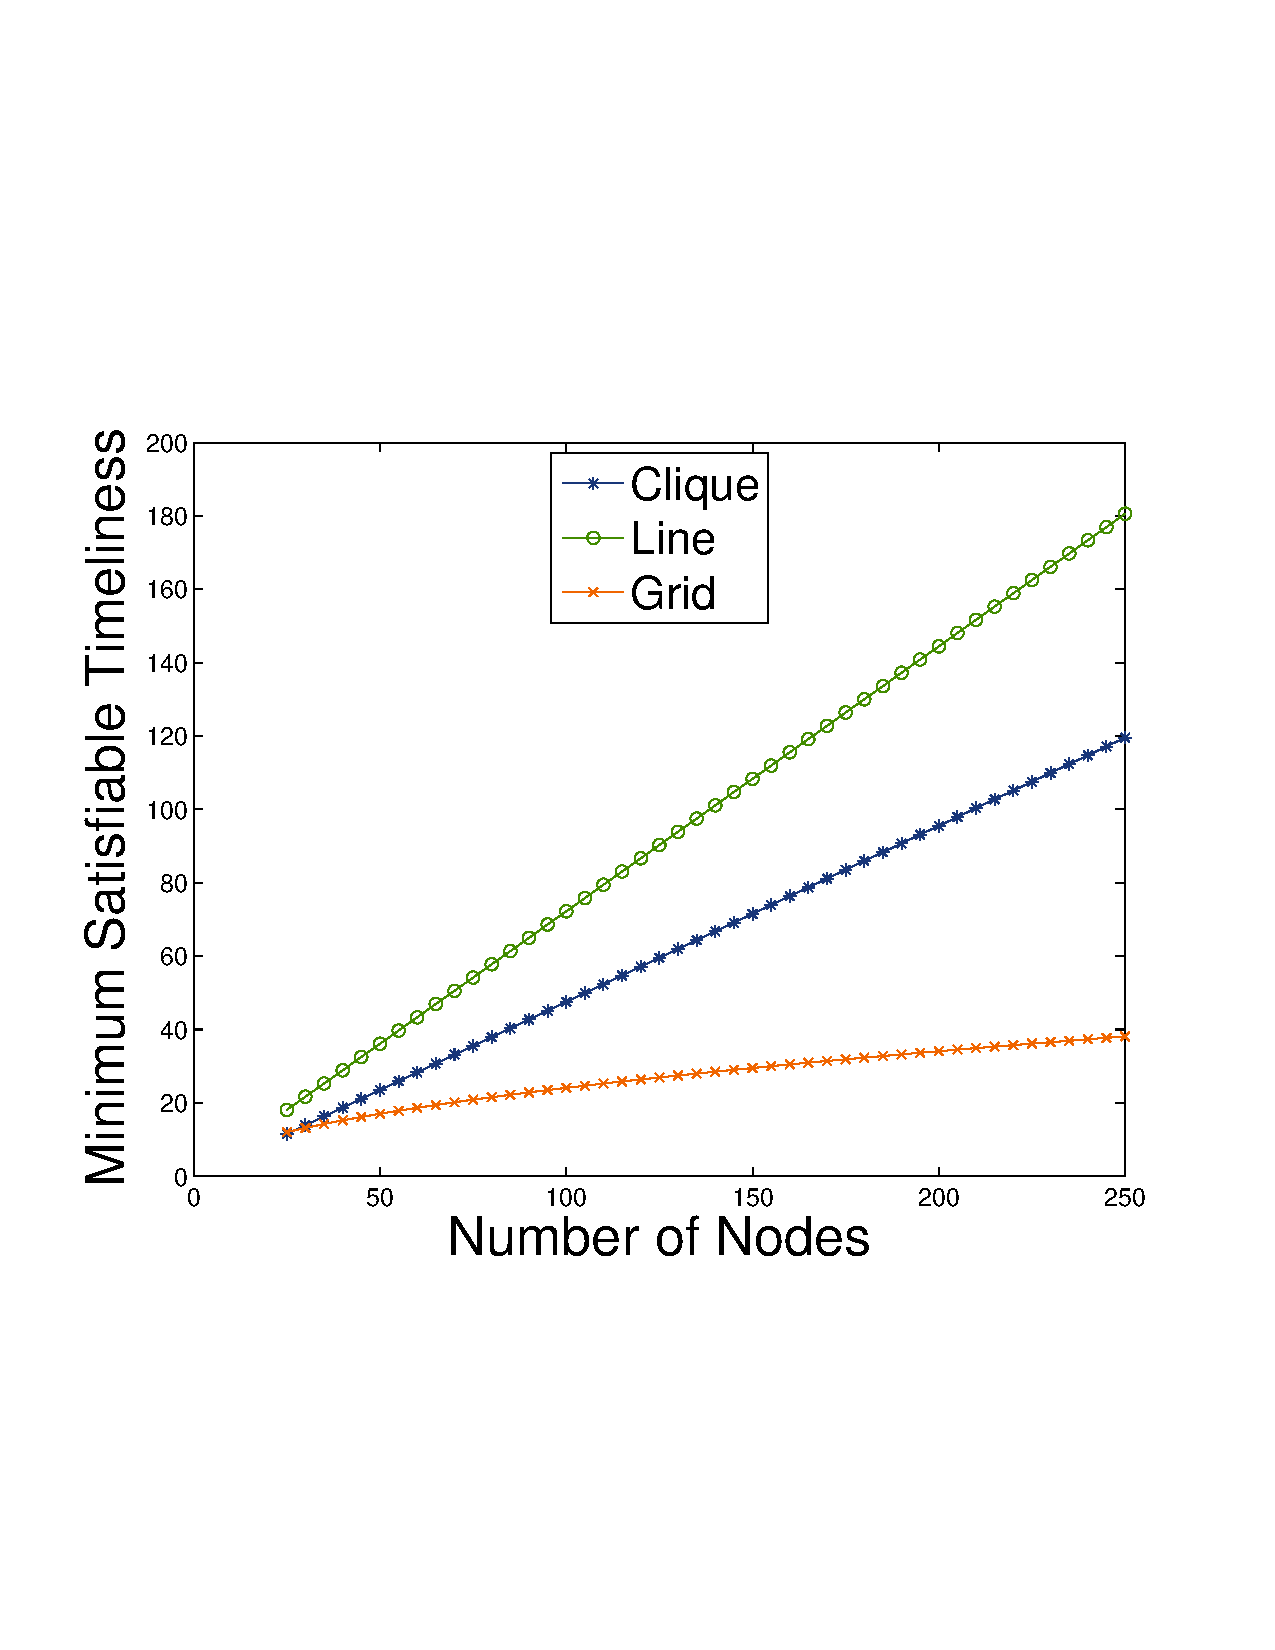
\includegraphics[scale=0.22, clip=true, trim=14mm 65mm 25mm 65mm]{figures/use_cases_examples/tness_vs_num_nodes_5_SS_12_IS_2_W_color.pdf}
        \label{fig:use_case_tness_vs_num_nodes}
        }
    \subfigure[Max Sum Sim. vs. Network Size (Timeliness = 50)]{
	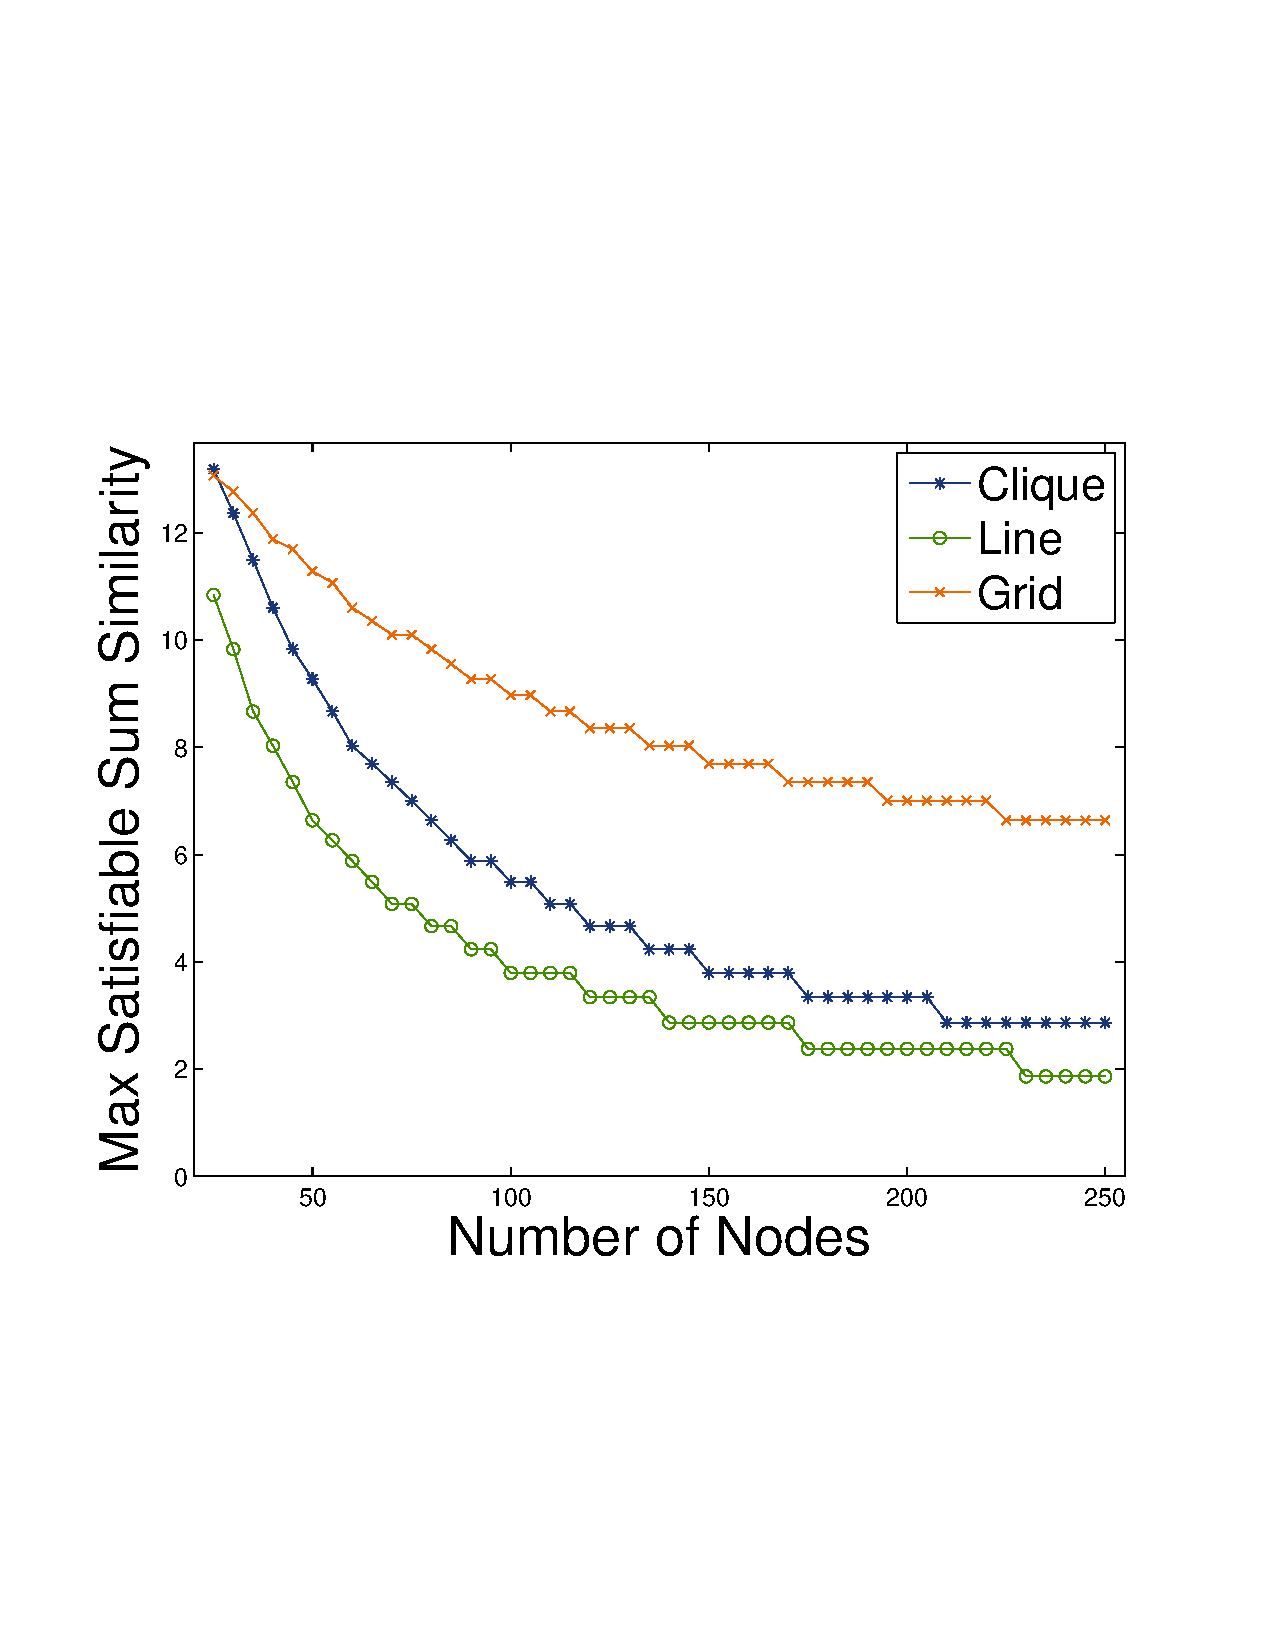
\includegraphics[scale=0.22, clip=true, trim=14mm 65mm 25mm 65mm]{figures/use_cases_examples/sum_sim_vs_num_nodes_50_T_12_IS_2_W_color.pdf}
        \label{fig:use_case_sum_sim_vs_num_nodes}
        }
  \subfigure[Max Network Size vs. Sum Sim. (Timeliness = 10)]{
	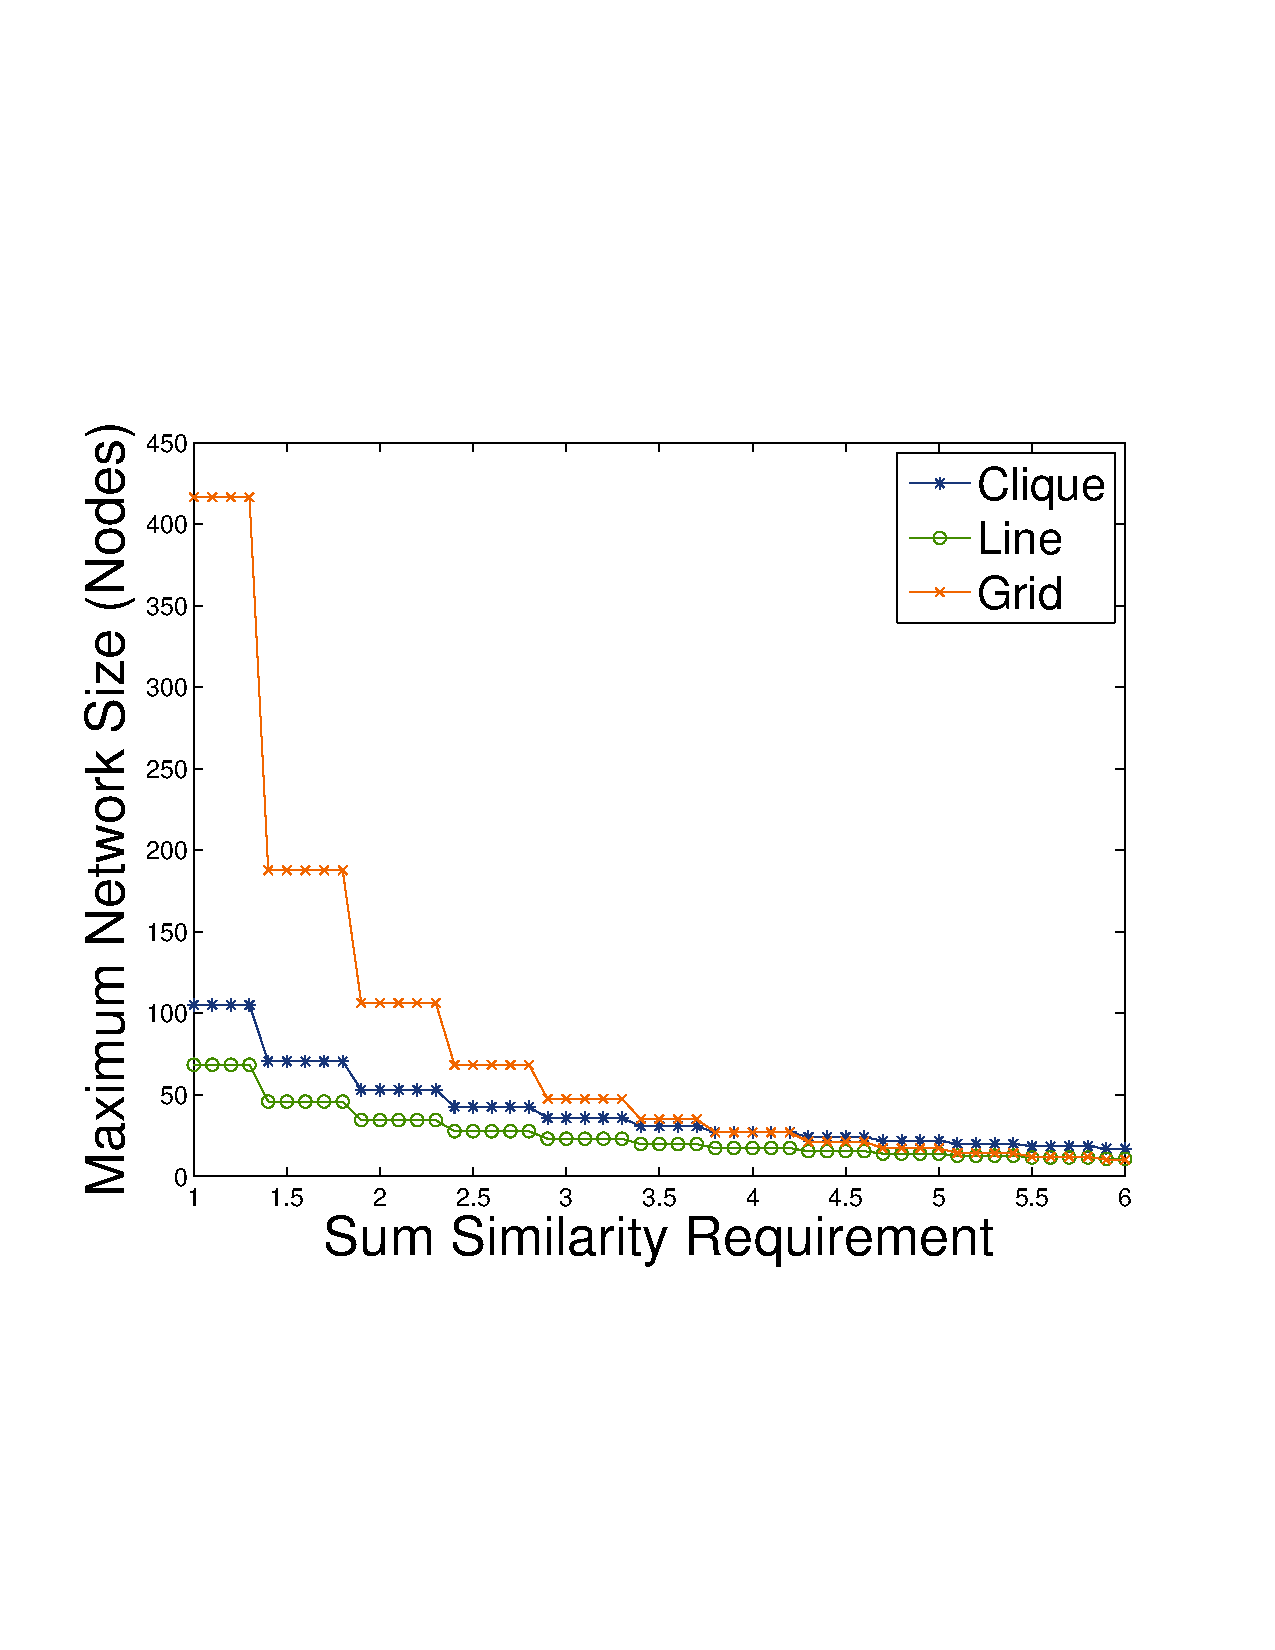
\includegraphics[scale=0.22, clip=true, trim=14mm 65mm 25mm 65mm]{figures/use_cases_examples/num_nodes_vs_sum_sim_10_T_12_IS_color.pdf}
        \label{fig:use_case_num_nodes_vs_qoi}
        }
  \subfigure[Max Network Size vs. Timeliness (Sum Sim. = 5.0)]{
	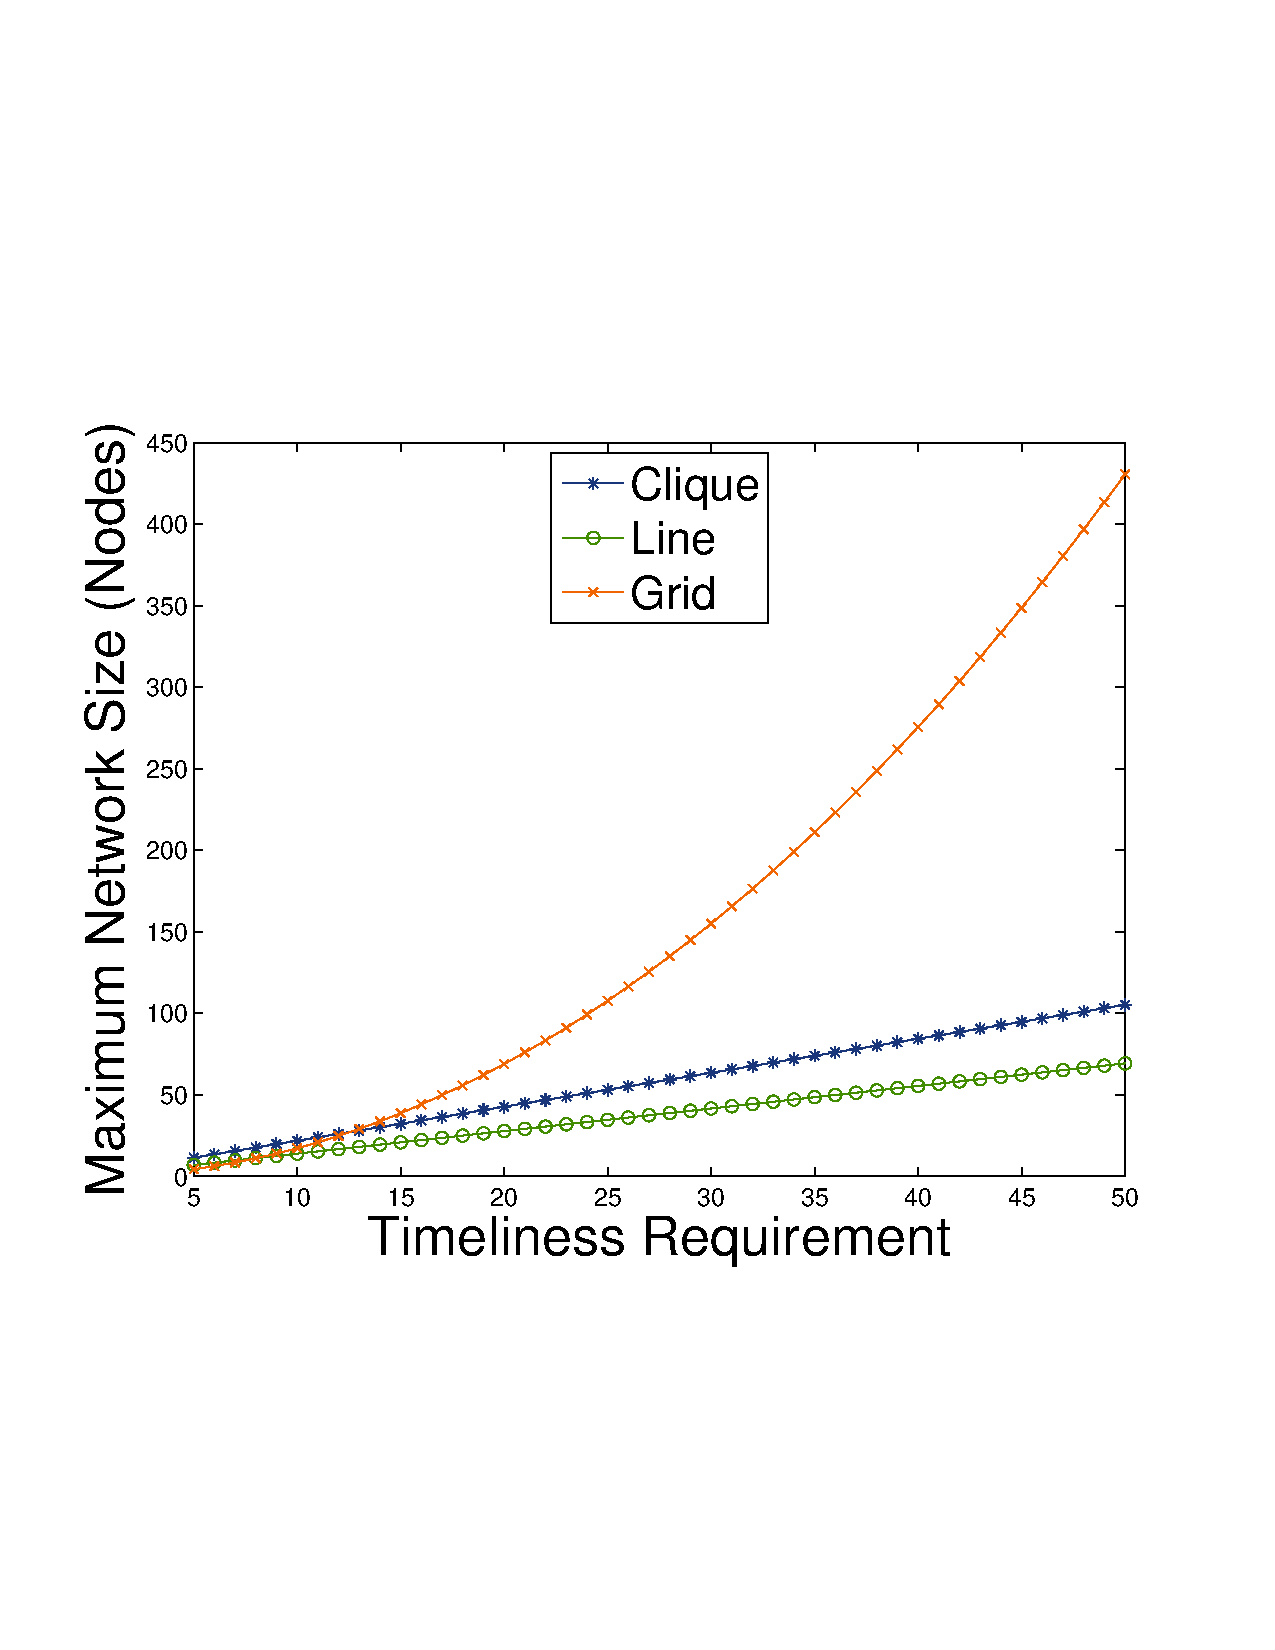
\includegraphics[scale=0.22, clip=true, trim=14mm 65mm 25mm 65mm]{figures/use_cases_examples/num_nodes_vs_tness_5_SS_12_IS_color.pdf}
        \label{fig:use_case_num_nodes_vs_qoi_2}
        }
   \vspace{-1mm}
   \caption{Varying design parameters provide immediate limitations as well as evident trends and comparisons.}
   \label{fig:huh_net_design}
   \vspace{-6mm}
\end{figure*}
 
Now that we have established a model for QoI satisfiability and scalability and shown its accuracy in predicting estimated limits, we show how it can also provide quick, but useful intuition about the impact of various network parameters.  Once an equation for a network's limitations is formulated as was done for equations in Table \ref{table:scal_eqs} %(\ref{eq:clique_gen})-(\ref{eq:grid_gen})
, it can be solved for a single parameter to gain an understanding of its reliance on the other factors.  This analysis can be done very quickly and easily by approximating when appropriate, or by using symbolic and/or numerical solvers.  To exemplify this application in network design, we have applied this process to the equations in Table \ref{table:scal_eqs} % (\ref{eq:clique_gen})-(\ref{eq:grid_gen}) 
and created several figures that provide insight into network limitations and tradeoffs.

Figure \ref{fig:use_case_tness_vs_num_nodes} shows minimum satisfiable timeliness values for different topologies of increasing size.  While it may be intuitive that a grid network should be able to serve flows with lower timeliness constraints than a line network since it will have shorter average path lengths, what is not intuitive is \emph{how much} lower of a timeliness constraint is satisfiable.  Here, we see that a grid network can scale up to over $250$ nodes while supporting flows with $T = 40$.  A line network, on the other hand, can only scale to only approximately $20\%$ of that network size for the same timeliness value.  %In either case, it is intuitive to know how a clique network's timeliness satisfiability should respond to either a grid or line network since its operation is quite different.

Figure \ref{fig:use_case_sum_sim_vs_num_nodes} visualizes sum similarity limits for network instances with timeliness fixed.  Here, again, limits and trends are quickly evident.  In addition, the nonlinearity of completeness requirements are manifested here as the data requirements for the highest completeness requirements are only sustainable for small networks, but as the network size increases, the impact on achievable completeness is not as dramatic.  

%To highlight this example, we can refer back to Figure \ref{fig:topkAvgNumSameSet} and see that in order to obtain $7$ images matching the target image on average, we should collect $~28$ images, which we see from \ref{fig:topkSumSim} equates to a sum similarity of approximately $6.5$.  If we require a timeliness of $50$ seconds and our network topology has $50$ nodes that are in a line, a sum similarity of $6.5$ is the maximum completeness the network can support.  If these same nodes are arranged in a grid network, however, we see that the network still has the capability to support more traffic, closer to a sum similarity of $11.5$, which is twice as many images on average.

Finally, given a topology and application with predetermined requirements of $\mathbf{q}$, we may be simply interested in how large our network can grow before its capacity to deliver the desired QoI is no longer possible.  Values that answer this question are in Figures \ref{fig:use_case_num_nodes_vs_qoi} and \ref{fig:use_case_num_nodes_vs_qoi_2}.  Once again, the graphs show the major impact completeness and timeliness requirements can have on network size.  Figure \ref{fig:use_case_num_nodes_vs_qoi} especially shows the impact of using completeness instead of simply throughput as the non-linear relationship of completeness to data rate pointed out in Section \ref{sec:qoi_model} is evident here.

%In this section, we approximate where appropriate like in (\ref{eq:tness_line_1})-(\ref{eq:tness_line}) below since the insights we seek here are more easily gained with simpler expressions, and are not greatly affected for large values.  In applying the framework in practice, though, numerical solvers can be used, removing the need for approximation.    

%Throughout this section, channel rate and packet size values are again fixed at $W = 2$ Mbps and $P_S = 1,500$ Bytes.  Also, we again choose sum similarity as the illustrative metric of completeness, but any other definition of completeness could be swapped in here.  Specific values of $SS$, $T$, and $N$ are varied to show various effects, so their values are explicitly listed in each figure and/or description.

%\subsubsection{Timeliness}
%Since $\mathbf{q}$ is a composite requirement of both timeliness and sum similarity, the value representing completeness in this application, we can explore the limits and impact of network parameters on each separately.  First, we will substitute appropriate values for each topology, and then solve the inequality for $T$. The result for each is as follows:
%
%\vspace{4mm}
%\noindent
%Clique:
%\begin{equation}
%	T \geq \frac{B}{W} \cdot (N -1) + \frac{P_S}{W}
%\label{eq:tness_clique}
%\end{equation}
%Line:
%\begin{eqnarray}
%\label{eq:tness_line_1}
%	T &\geq& 1.5 \cdot \frac{B}{W} \cdot \frac{(N-1)^2}{N-2} + 1.5 \cdot \frac{P_S}{W} \cdot (\frac{N}{4} - 1) \\
%	&\approx& 1.5 \cdot \frac{B}{W} \cdot (N-1) + 1.5 \cdot \frac{P_S}{W} \cdot (\frac{N}{4} - 1)
%\label{eq:tness_line}
%\end{eqnarray}
%Grid:
%\begin{equation}
%	T \geq 5 \cdot \frac{\sqrt{N}}{W} \cdot (B + \frac{P_S}{3})
%\label{eq:tness_grid}
%\end{equation}

%Using these inequalities, not only can network designers gain estimates of maximum timeliness constraints satisfiable in various network scenarios, but they can also quickly compare the dependency on specific parameters.  By quick examination of these relationships, one can see that timeliness has a $O(N)$ relationship with respect to network size in clique and line topologies, but $O(\sqrt{N})$ in a grid topology.  Figure \ref{fig:use_case_tness_vs_num_nodes} reinforces this lesson.  The graph shows minimum $T$ values for increasing values of $N$ with all other values fixed, showing that a grid network can serve tighter timeliness constraints than other topologies in larger networks.

%While it may have been intuitive that a grid network should be able to serve flows with lower timeliness constraints than a line network since it will have shorter average path lengths, what is not intuitive is \emph{how much} lower of a timeliness constraint is satisfiable.  For example, we see here that a grid network can scale up to over $250$ nodes while supporting flows with $T = 40$.  A line network, on the other hand, can only scale to only approximately $20\%$ of that network size for the same timeliness value.  In either case, it is intuitive to know how a clique network's timeliness satisfiability should respond to either a grid or line network since its operation is quite different.  With the inequalities in (\ref{eq:tness_clique})-(\ref{eq:tness_grid}), though, it is quickly and easily understood.

%\begin{figure}[ht]
%\centering
%\subfigure[Achievable Timeliness vs. Network Size for a fixed Sum Similarity = 5.0]{
%	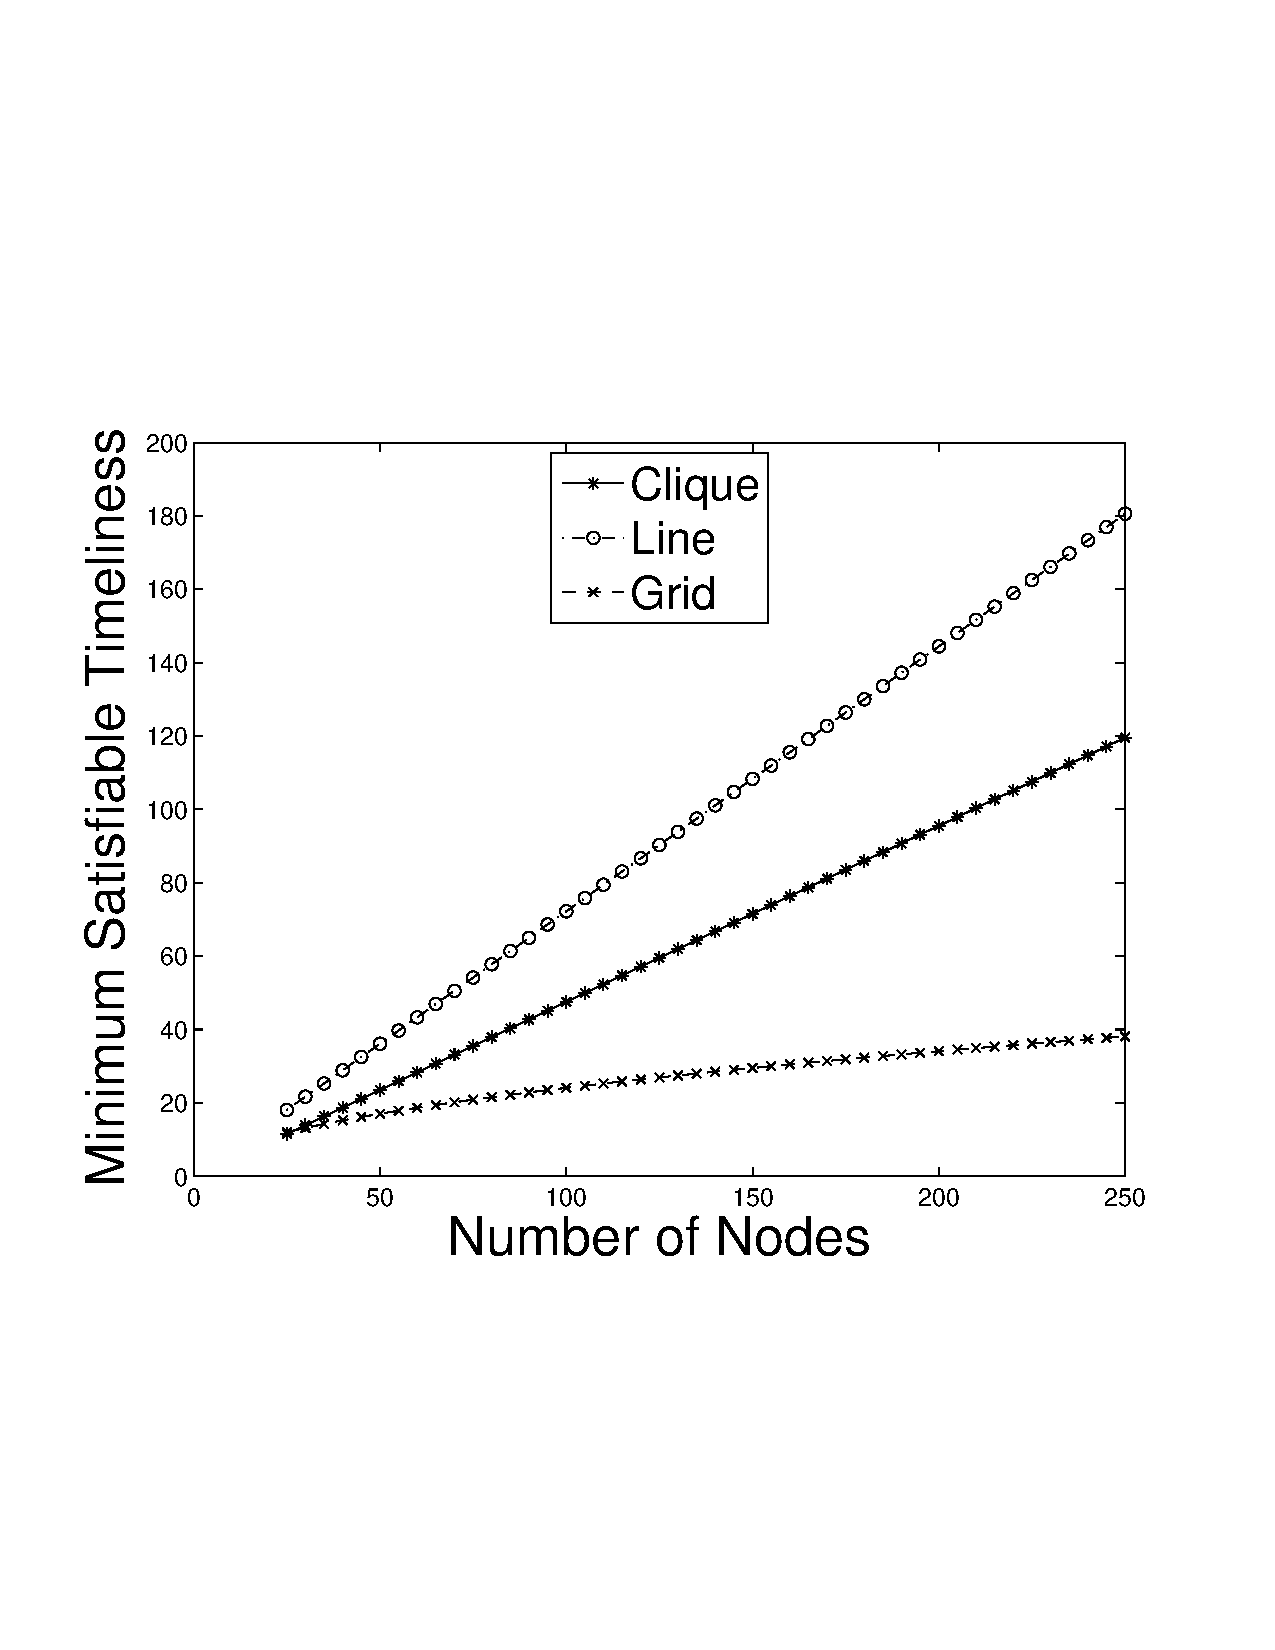
\includegraphics[scale=0.31, clip=true, trim=15mm 65mm 20mm 65mm]{figures/use_cases_examples/tness_vs_num_nodes_5_SS_12_IS_2_W.pdf}
% 	\label{fig:use_case_tness_vs_num_nodes}
%	}
%\subfigure[Achievable Sum Similarity vs. Network Size for a fixed Timeliness = 50]{
%	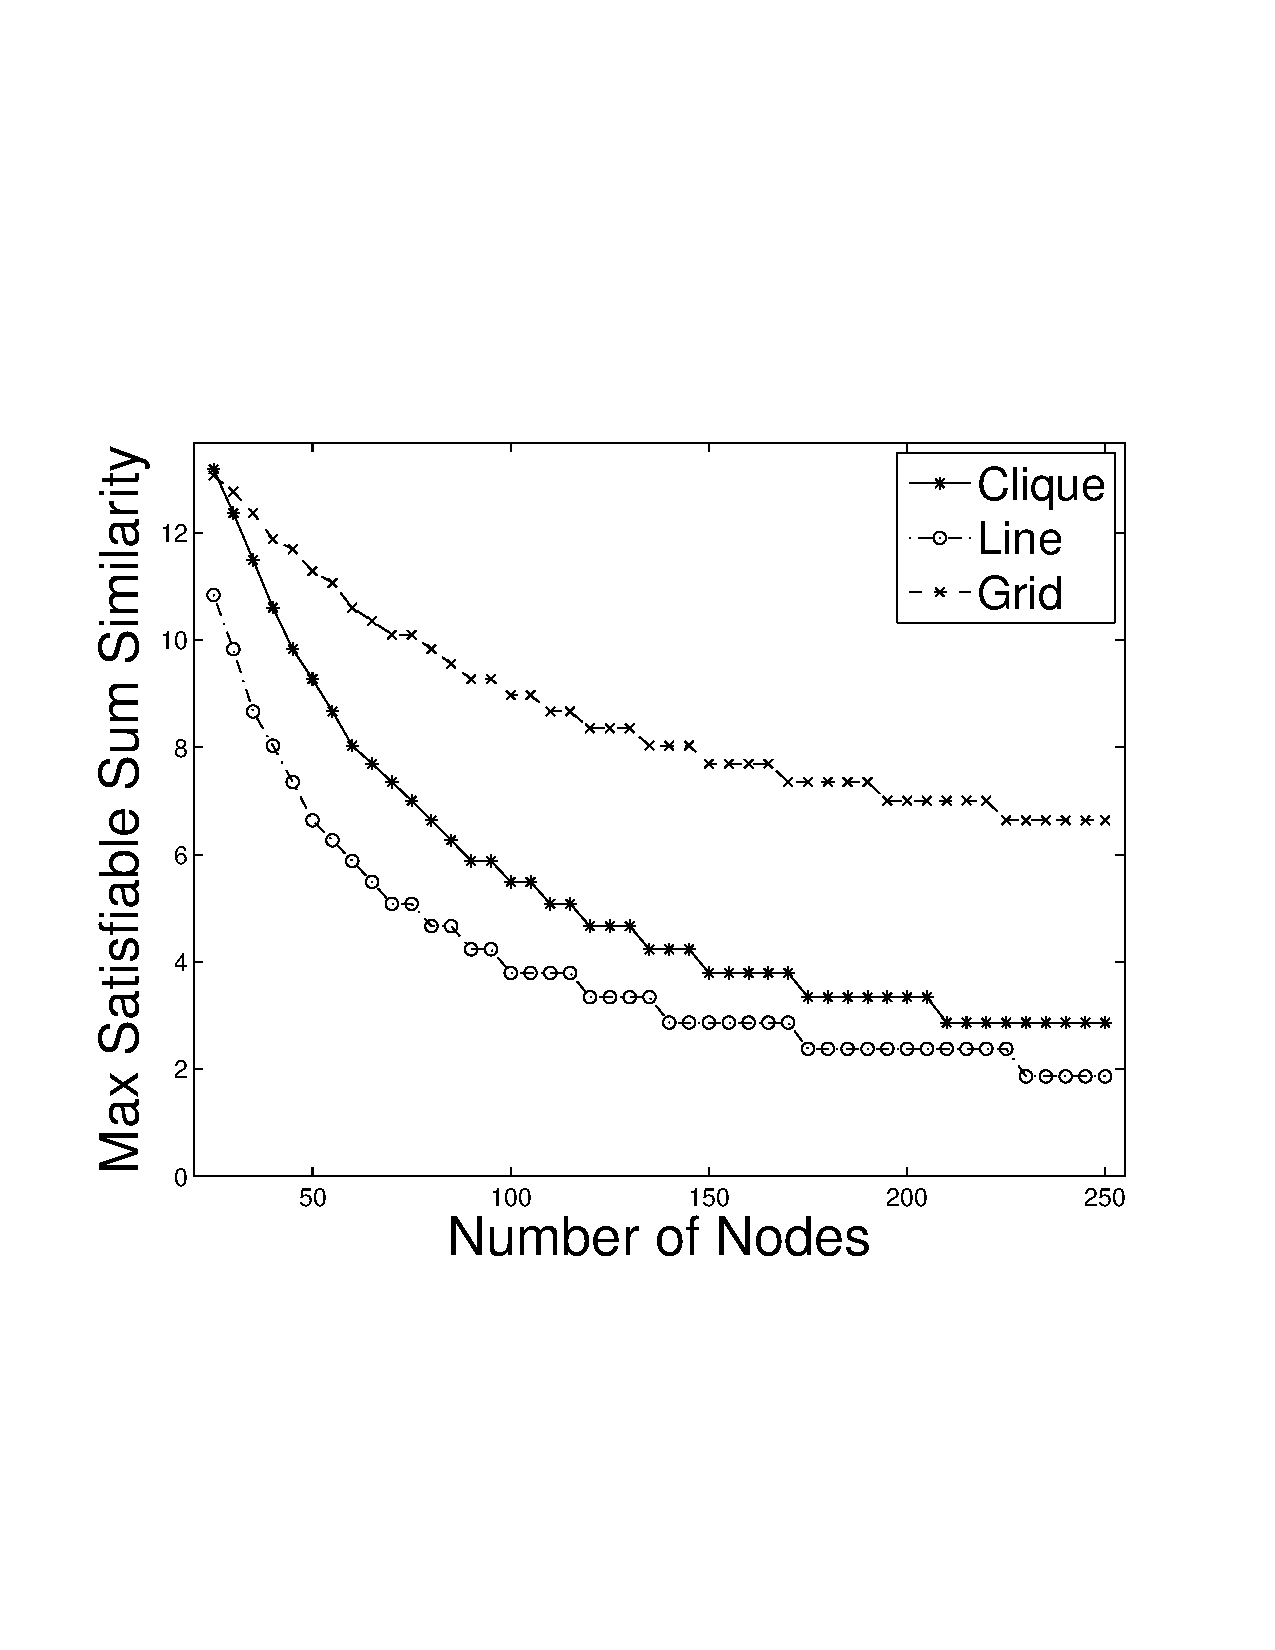
\includegraphics[scale=0.31, clip=true, trim=15mm 65mm 20mm 65mm]{figures/use_cases_examples/sum_sim_vs_num_nodes_50_T_12_IS_2_W.pdf}
%	\label{fig:use_case_sum_sim_vs_num_nodes}
%	}
%\caption{Achievable QoI values are quickly evident for various network sizes and comparisons between topologies are easily made.}
%\vspace{-2mm}
%\end{figure}
%
%\begin{figure}[ht]
%\centering
%  \subfigure[Varying Sum Similarity (T = 10)]{
%	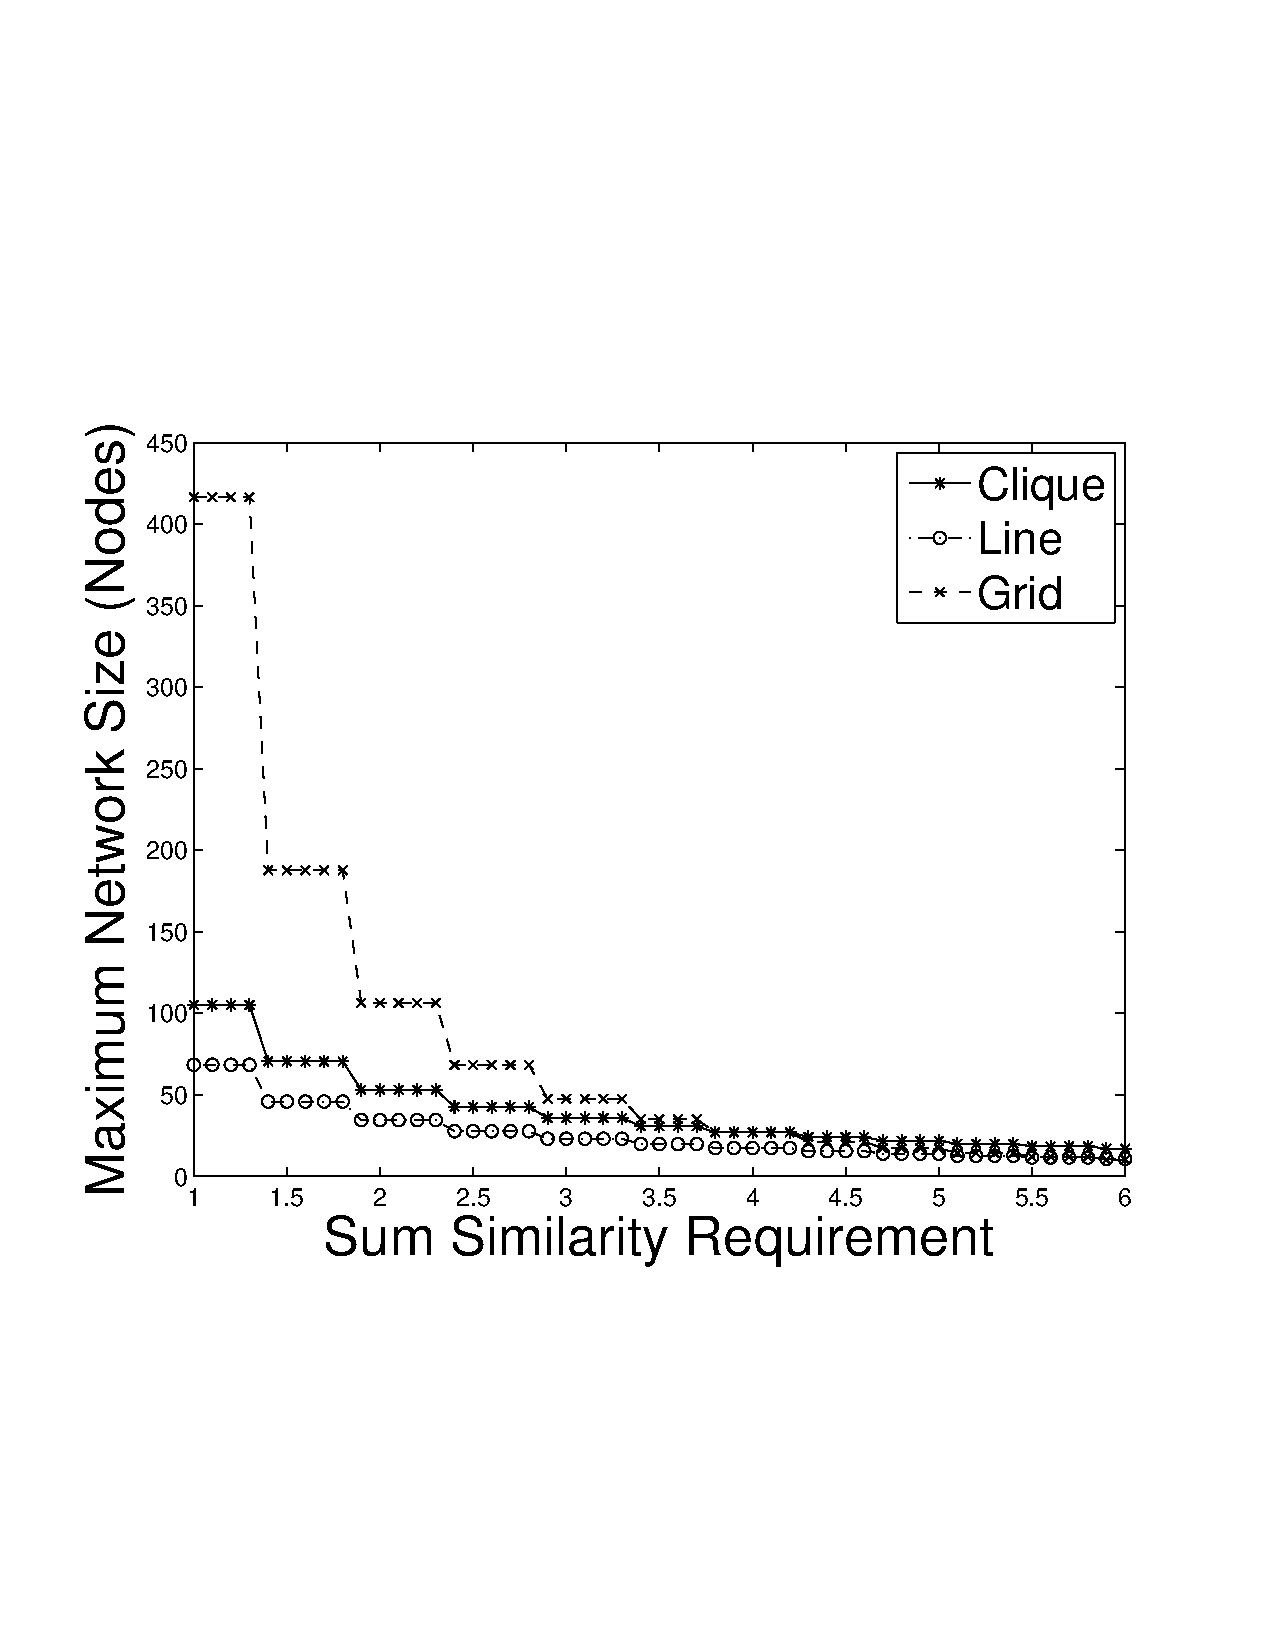
\includegraphics[scale=0.31, clip=true, trim=15mm 65mm 20mm 65mm]{figures/use_cases_examples/num_nodes_vs_sum_sim_10_T_12_IS.pdf}
%	}
%  \subfigure[Varying Timeliness (SS = 5.0)]{
%	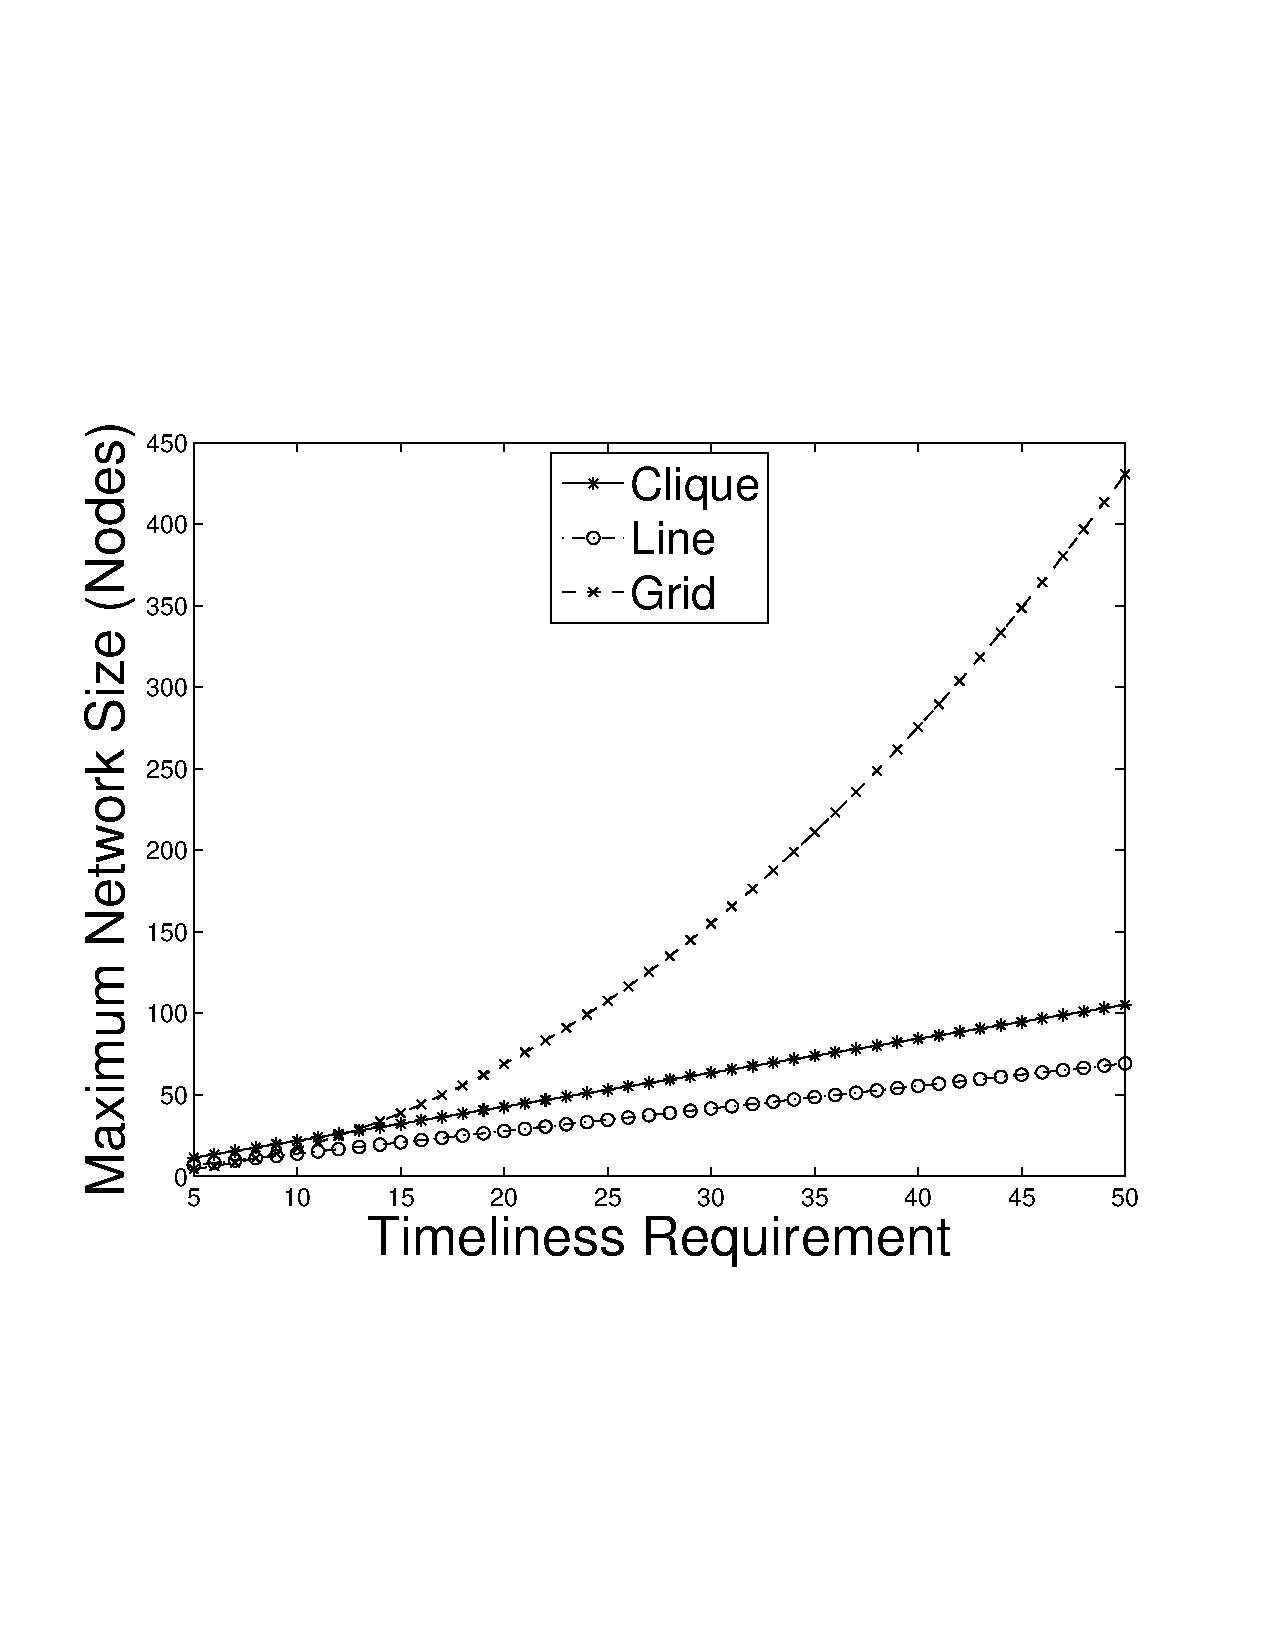
\includegraphics[scale=0.31, clip=true, trim=15mm 65mm 20mm 65mm]{figures/use_cases_examples/num_nodes_vs_tness_5_SS_12_IS.pdf}
%	}
%\caption{Achievable Network Size for Varying QoI Requirements}
% \label{fig:use_case_num_nodes_vs_qoi}
%    \vspace{-7mm}
%\end{figure}

%\subsubsection{Sum Similarity (Completeness)}
%
%In the exact same manner, we can evaluate maximum sum similarity values, $SS$, achievable by a network.  To do so, we define the inverse of the function $Q(SS) = k_{req}$ defined above.  Here, $Q'(k_{req}) = SS$ provides the sum similarity corresponding to the number of images served in each flow.  The relationship for sum similarity for each topology is described with the following relations:
%
%\vspace{4mm}
%\noindent
%Clique:
%\begin{equation}
%	SS \leq Q'( \frac{W \cdot T - P_S}{I_s \cdot (N-1)} )
%\end{equation}
%Line:
%\begin{equation}
%	SS \leq Q'( \frac{W \cdot T - 1.5 \cdot P_S \cdot (\frac{N}{4} - 1)}{3 \cdot I_s \cdot \frac{(N-1)^2}{2(N-2)}} )
%\end{equation}
%Grid:
%\begin{equation}
%	SS \leq Q'( \frac{W \cdot T - 2.5 \cdot P_S \cdot (\frac{2}{3} \cdot \sqrt{N} - 1)}{5 \cdot I_s \cdot \sqrt{N}} )
%\end{equation}
%
%Figure \ref{fig:use_case_sum_sim_vs_num_nodes} visualizes these sum similarity limits for network instances of different numbers of nodes while timeliness is fixed.  Here, again, limits and trends are quickly evident.  In addition, the nonlinearity of completeness requirements are manifested here as the data requirements for the highest completeness requirements are only sustainable for small networks, but as the network size increases, the impact on achievable completeness is not as dramatic.  
%
%To highlight this example, we can refer back to Figure \ref{fig:topkAvgNumSameSet} and see that in order to obtain $7$ images matching the target image on average, we should collect $~28$ images, which we see from \ref{fig:topkSumSim} equates to a sum similarity of approximately $6.5$.  If we require a timeliness of $50$ seconds and our network topology has $50$ nodes that are in a line, a sum similarity of $6.5$ is the maximum completeness the network can support.  If these same nodes are arranged in a grid network, however, we see that the network still has the capability to support more traffic, closer to a sum similarity of $11.5$, which is twice as many images on average.
% 
%\subsubsection{Scalability}
%
%Finally, given a topology and application with predetermined requirements of $\mathbf{q}$, we may be simply interested in how large our network can grow before its capacity to deliver the desired QoI is no longer possible.  The proper relationships to answer this question are below in (\ref{eq:scal_clique})-(\ref{eq:scal_grid}), and Figure \ref{fig:use_case_num_nodes_vs_qoi} gives maximum scalability examples when either component of $\mathbf{q}$ is varied.  Once again, the graphs show the major impact completeness and timeliness requirements can have on network size.
%
%\vspace{4mm}
%\noindent
%Clique:
%\begin{equation}
%	N \leq \frac{W \cdot T - P_S}{B} -1
%\label{eq:scal_clique}
%\end{equation}
%Line:
%%\begin{equation}
%%	W \cdot T - 3 \cdot B \cdot \frac{(N-1)^2}{2(N-2)} - 1.5 \cdot P_S \cdot (\frac{N}{4} - 1)
%%\end{equation}
%%\indent which can be approximated to:
%\begin{equation}
%	N \leq \frac{W \cdot T + \frac{3}{2}P_S}{\frac{3}{2}B+\frac{3}{8}P_S}
%\label{eq:scal_line}
%\end{equation}
%Grid:
%\begin{equation}
%	N \leq (\frac{W \cdot T}{5 \cdot B + \frac{5}{3} \cdot P_S})^2
%\label{eq:scal_grid}
%\end{equation}




\section{Scalably Feasible QoI Regions}
\label{sec:scal_feasible_qoi}

In some applications, the data requirements to achieve a certain level of QoI may include a minimum number of nodes or sources in addition to the size of the data load that must be served.  For example, a system may require that each image must come from a different node, perhaps because each node only has one image or maybe by design to provide increased credibility through corroboration, another contextual metric of interest in QoI-aware networks.  We will use this example to illustrate an interesting observation that arises in such scenarios.
% may imply that a certain number of nodes afre required to achieve a desired level of QoI.  For example, a system may require $k_{req}$ images from $n$ different nodes.  

%Now let us consider a special case where nodes collect a total of $k_{req}$ images, but each image must come from a different node, perhaps because each node only has one image or maybe by design to provide increased credibility through corroboration, another contextual metric of interest in QoI-aware networks. This scenario allows us to illustrate an interesting observation.  

Let us assume that we are designing a surveillance network with nodes arranged in a grid and one data sink in the corner of the network.  This data sink node issues queries with a set of QoI requirements that include completeness and timeliness, $\mathbf{q} = \{C,T\}$, but this completeness must be met while only allowing one image per source node.  With this traffic model, we can derive a maximum traffic factor and create a scalability equation for this particular scenario.

Here, the data sink node will have two neighbors through which all queries will be forwarded, so clearly we can choose either of these to consider as the bottleneck node.  Even if the network balances traffic evenly over both of these nodes, each must forward at least $\frac{N-1}{2}-1$ since there are $N-1$ sources, half of which must be forwarded through each of the data sink's two neighbors, excluding the $1$ image from each of these neighbors themselves.  If we assume these queries may be simultaneously served in the worst case, then we can simply use this expression for the maximum Traffic Factor.  Then, using the same values derived for a grid network in Table \ref{table:rf_ff_sf_values} in place of the other factors in Equation (\ref{eq:general_scal}), we get the following scalability equation:

\begin{equation}
	W \cdot T - 5 \cdot I_s \cdot (\frac{N-1}{2}-1) - 2.5 \cdot P_s \cdot 2 \sqrt{N} \geq 0
\end{equation}

%Consider a set of QoI requirements that include completeness and timeliness, $\mathbf{q} = \{C,T\}$.  As previously noted, a certain number of images are required to achieve this desired level of completeness, $Q(C) = k_{req}$.  Unlike the model used in Section \ref{sec:network_design}, however, each node can contribute only one image to $k_{req}$, which implies a minimum network size of $N \geq k_{req}$ in order to achieve the completeness outlined in the QoI requirements.  On the other hand, applying derived scalability equations to this network, we can determine the maximum network size, which we will call $N_{max}$ here for distinction.  
From this equation, we can determine the maximum network size, which we will call $N_{max}$ here.  However, the specified restriction that each node can contribute only one image to $k_{req}$ implies a minimum network size of $N \geq k_{req}$ in order to achieve the completeness outlined in the QoI requirements. 

These two facts are important, because when $N_{max} < k_{req}$, then it is not possible to provide the QoI level $\mathbf{q}$.  Hence, this set of QoI requirements is infeasible, or \emph{scalably infeasible}.  This phenomenon defines the concept of a \emph{Scalably Feasible QoI Region}, which refers to the region in which sets of QoI pairs can be supported with the given network signature.  

\begin{figure}[ht]
\centering
	\subfigure[The curved plane represents maximum scalability, and the flat plane represents minimum required images.  Therefore, all (Sum Sim., Timeliness) pairs to the right of the intersecting red line are within the scalably feasible QoI region.]
	{
		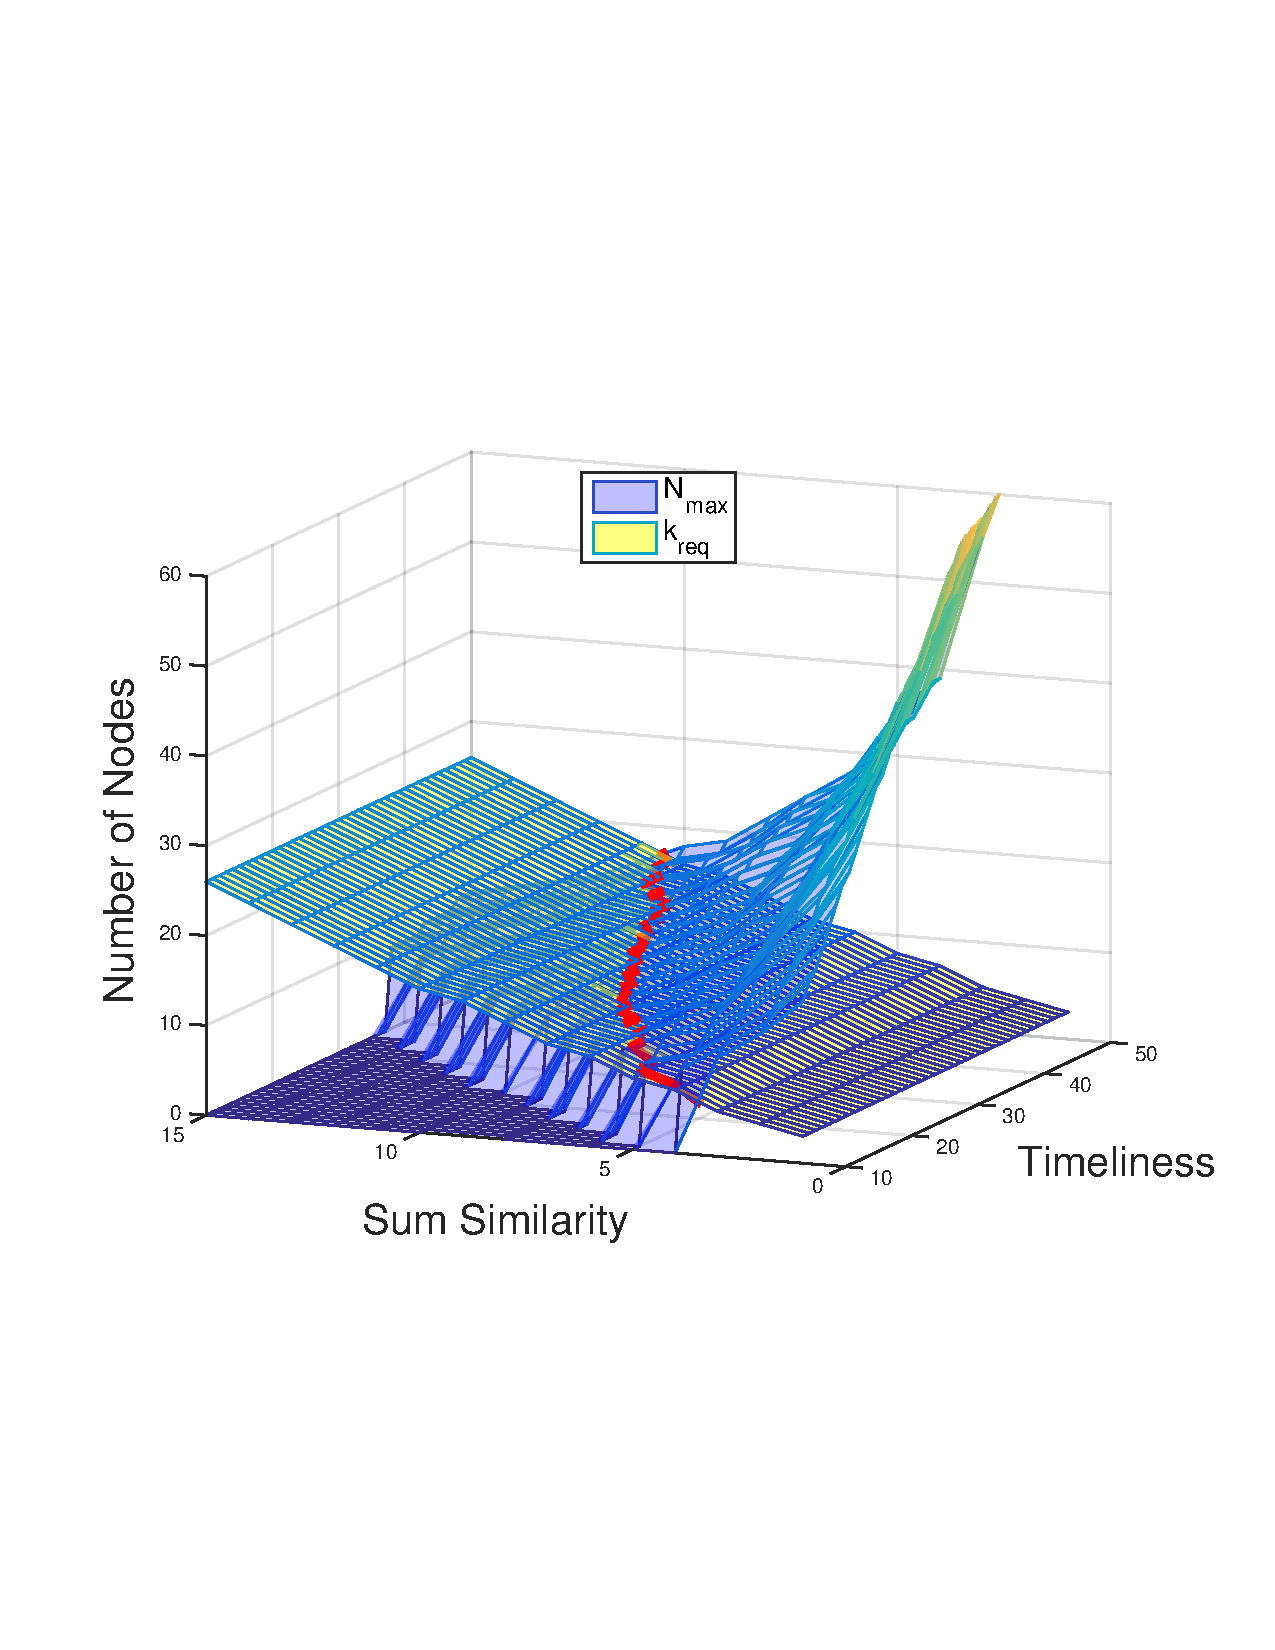
\includegraphics[scale=0.31, clip=true, trim=10mm 65mm 10mm 77mm]{figures/scal_feas_qoi/scal_feas_qoi_corner_sink_6.pdf}
		 \label{fig:scal_feasible_region_3d}
	 }
	
	\subfigure[The shaded region represents feasible values of QoI (Completeness, Timeliness pairs) - a 2-d projection from Figure \ref{fig:scal_feasible_region_3d}]
	{
		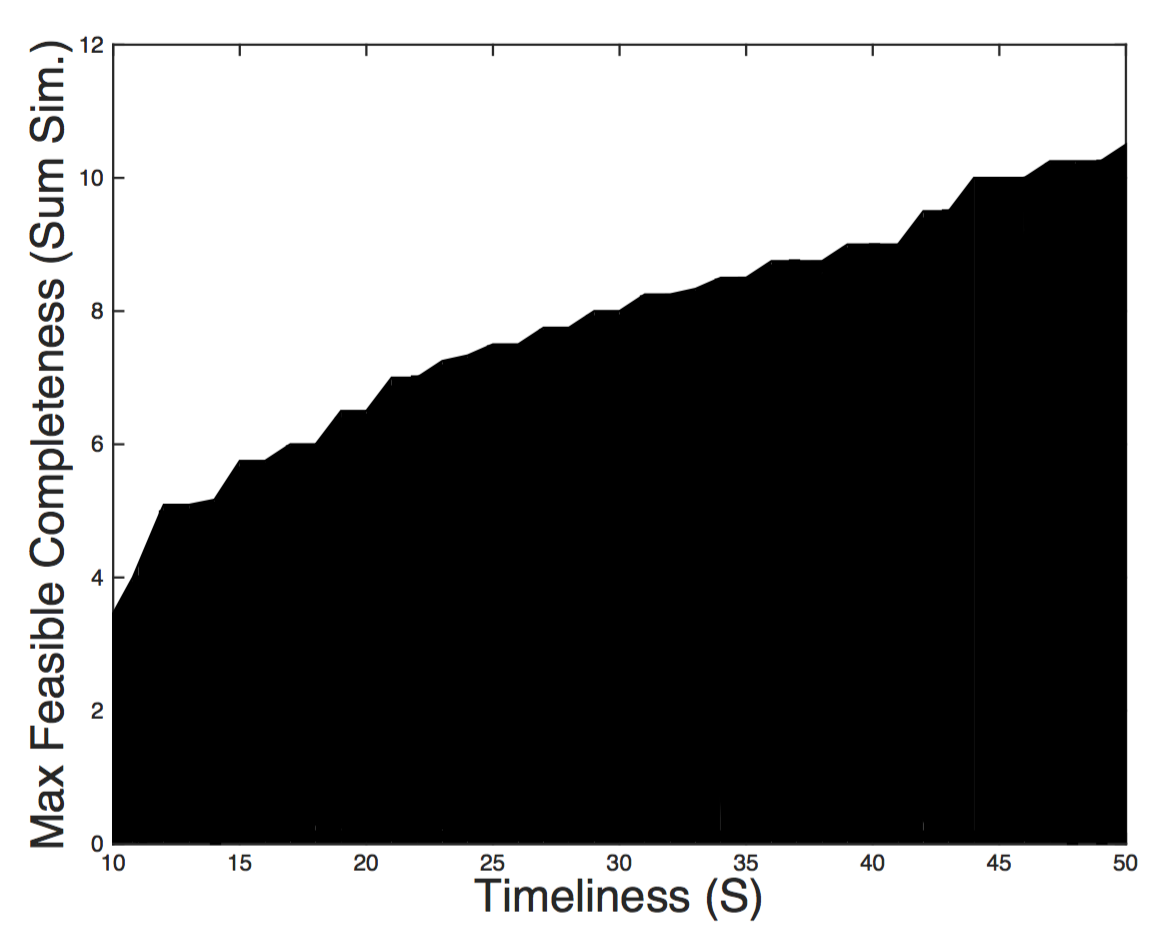
\includegraphics[scale=0.14, clip=true, trim=0mm 0mm 0mm 0mm]{figures/scal_feas_qoi/scal_feas_qoi_grid_corner_sink_2d_2.png}
		\label{fig:scal_feasible_region_2d}
	}
	\caption{Graphical representations of the \emph{Scalably Feasible QoI Region}}
	\label{fig:scal_feasible_region}
\end{figure}

Figure \ref{fig:scal_feasible_region_3d} provides a visual representation of this region for a grid network that institutes the given traffic model.
Here, $N_{max}$, calculated for QoI requirements of Sum Similarity over the range $[1, 15]$ and Timeliness over the range $[10, 50]$,
is shown in the graph by the blue surface.  On the same graph is the number of images required, $k_{req}$, for each Sum Similarity requirement, shown with the yellow surface on the graph.  The intersection of these two surfaces, displayed with a red line, provides the edge of the scalably feasible QoI region.  In this example, only QoI pairs to the right of this line, i.e. the region where $N_{max} > k_{req}$, are scalably feasible.  Figure \ref{fig:scal_feasible_region_2d} shows this same scalably feasible QoI region in two dimensions, projecting the region onto the x-y plane.  In this figure, the shaded region represents all valid pairs of completeness and timeliness requirements.

In general, regardless of how many images a node can contribute to a query response, it is possible to analyze the trade-off between different QoI attributes for a fixed value of maximum network size, $N_{max}$.  Specifically, by fixing $N$ in Table \ref{table:scal_eqs}, one can obtain $T$ and $k_{req}$ (and, hence, $C$) resulting in the set of supportable $\{C,T\}$ pairs defining a feasible region for QoI. This region can be visualized by intersecting the blue scalability curved plane with a flat surface fixed at $N_{max}$ instead of the yellow surface in Figure \ref{fig:scal_feasible_region}.  The scenario given in this section goes one step further and also takes into account  the network size actually required to generate/support a given QoI requirement (using the non-flat yellow surface derived from experimental results in Figure \ref{fig:scal_feasible_region_3d}).


%\section{Finding Bottleneck Flow}
\label{sec:bottleneck}

Again, we turn to the satisfiability equation, but use random variables for the Traffic Factor and Path Length, $TF_i$ and $PL_i$, respectively:
\begin{equation}
	T \geq \frac{ k_{req} \cdot I_S \cdot CF \cdot TF_i}{W} + \frac{P_S \cdot DF \cdot (PL_i-1)}{W}
\end{equation}
where we will call the total delay
\begin{equation}
	D_i = \frac{ k_{req} \cdot I_S \cdot CF \cdot TF_i}{W} + \frac{P_S \cdot DF \cdot (PL_i-1)}{W}
\end{equation}

Now, we want to identify which flow $i$, identified by its origin node, is most likely to be the flow that cannot be satisfied in the allotted timeliness.  To do so, we can simply find the value of $i$ that results in the largest $D_i$.

\begin{figure}
\begin{centering}
    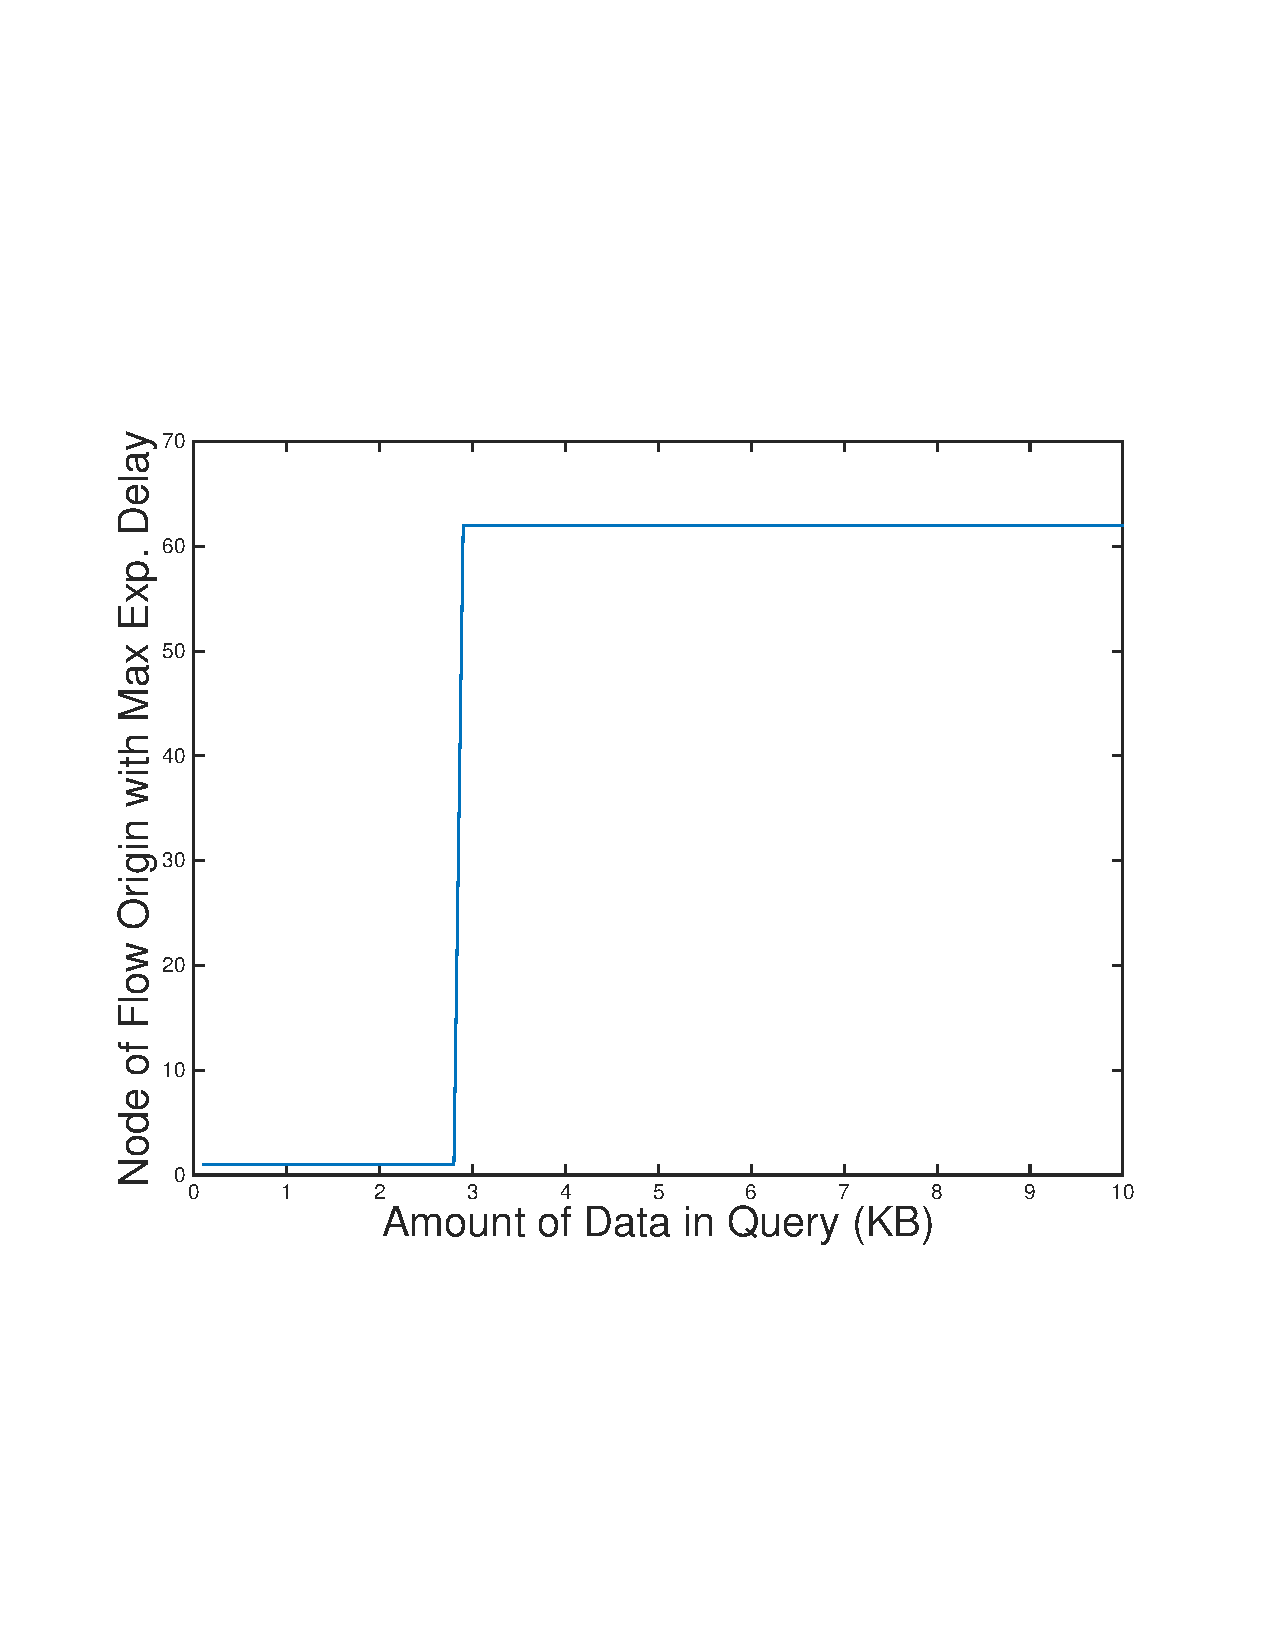
\includegraphics[scale=0.4, clip=true, trim=15mm 65mm 20mm 65mm]{figures/max_i_line_net_125.pdf}
    \caption{The value of $i$ (origin of a flow) that causes the maximum expected delay.}
    \label{fig:max_i_line_net}
\end{centering}
\end{figure}

Using the expected values for $TF_i$ and $PL_i$ from Figures \ref{fig:EV_TF_line_net} and \ref{fig:mean_PL_each_node_line_net}, we find the value of $i$ that maximizes $D_i$ for different data requirements, $B = k_{req}*I_S$.  Figure \ref{fig:max_i_line_net} shows that for low data requirements, the delay of multi-hop paths dominates, causing the ``Bottleneck" flow to be those that originate in node $1$ and have a larger expected path length.  At a point, though, as the amount of data required in the query grows, congestion will be the limiting factor in the network, making the Traffic Factor more important.  Thus, the node near the center of the network which will be likely to experience the highest amount of congestion become the source of flows with the highest delay.  In this case, we have $i = 62$, since the network has $125$ nodes (NOTE: It should probably be 63, but there is an ``off-by-one" error here because the definitions/formulations are not carefully derived to be correct on the boundaries).



%\section{Probability of Satisfying Query}
\label{sec:prob_sat}

Now, we have an expression for delay that is built up using random variables for the values of $TF$ and $PL$.  The next useful formulation is providing an expression that describes the probability of a bottleneck flow satisfying its timeliness requirement considering the underlying distributions.  With this formulation, we can define scalability as a network in which the flow's probability of satisfiability exceeds some threshold $P_{thresh}$:
\begin{equation}
	P(D_i < T) \geq P_{thresh}
\end{equation}

Once again, we have our total delay equation of a flow originating in node $i$:
\begin{equation}
	D_i = \frac{ k_{req} \cdot I_S \cdot CF \cdot TF_i}{W} + \frac{P_S \cdot DF \cdot (PL_i-1)}{W}
\end{equation}
Let us define two constants to simplify the expression:
\begin{eqnarray*}
	C_1 = \frac{k_{req} \cdot I_S \cdot CF}{W} \\
	C_2 = \frac{P_S \cdot DF}{W}
\end{eqnarray*}
Then, we can express the delay as
\begin{equation}
	D_i = C_1 \cdot TF_i + C_2 \cdot PL_i
\end{equation}
As we showed in the last section, we can determine $i$ using the expected values for $TF_i$ and $PL_i$, so assuming that we adopt this value of $i$, we can drop the notation:
\begin{equation}
	D = C_1 \cdot TF + C_2 \cdot PL
\end{equation}

\begin{eqnarray}
\nonumber
	f_{TF}^i (tf) = &&\frac{i}{N} \cdot \mathcal{N}(\mu(i),\sigma(i))  \\ \nonumber
			   &+& \sum\limits_{k=i}^{\frac{N}{2}-1} \cdot \frac{\frac{1}{2}-\frac{i}{N}}{\frac{N}{2} - i}\mathcal{N}(\mu(k),\sigma(k))  \\
			   &+& \frac{1}{2} \cdot \mathcal{N} (\mu(\frac{N}{2}),\sigma(\frac{N}{2}))
\label{eq:full_PDF_TF}
\end{eqnarray}











%\begin{figure}
%\begin{centering}
%    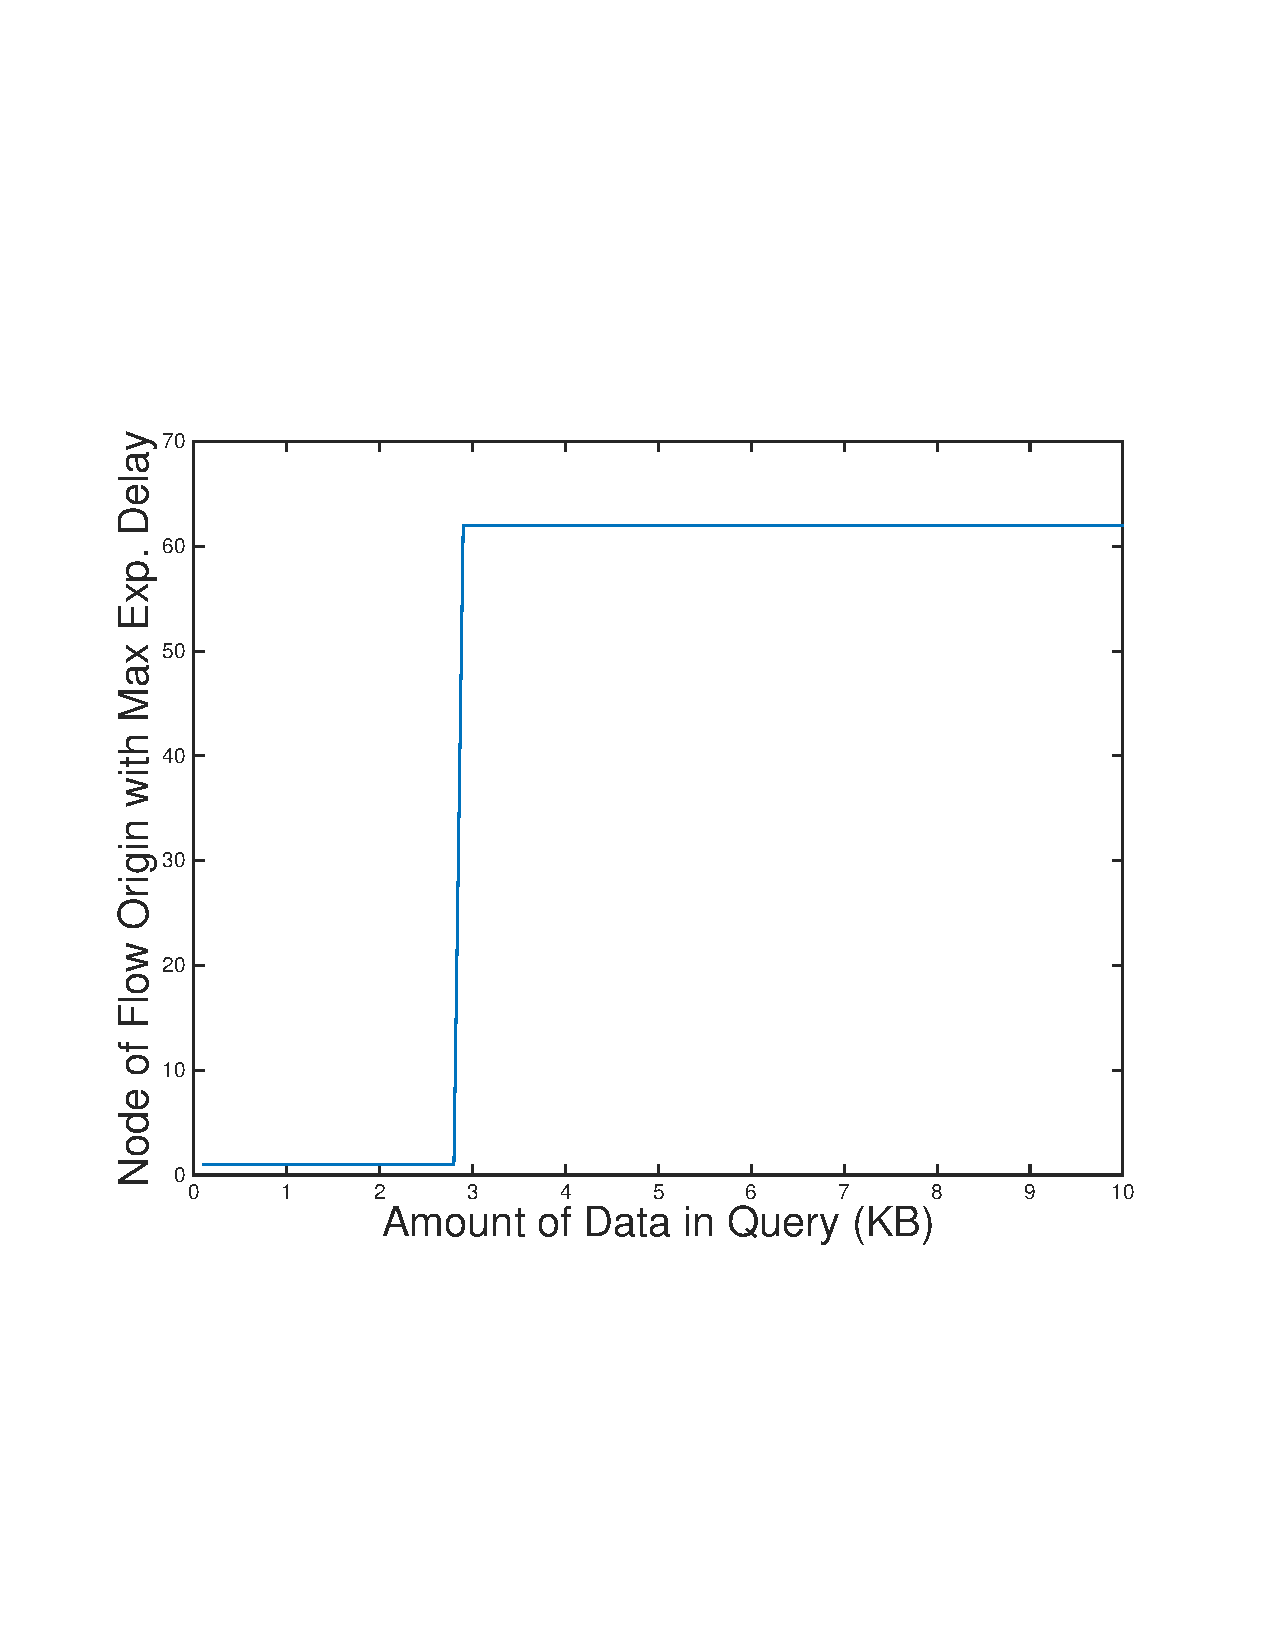
\includegraphics[scale=0.4, clip=true, trim=15mm 65mm 20mm 65mm]{figures/max_i_line_net_125.pdf}
%    \caption{The value of $i$ (origin of a flow) that causes the maximum expected delay.}
%    \label{fig:max_i_line_net}
%\end{centering}
%\end{figure}




\section{Discussion}
\label{sec:discussion}

%Given the coarseness of the model and the abstraction of many details, we note that the above is not a perfect predictor of a real network's capabilities. However, we show with packet-based, multi-hop simulation results in Section \ref{sec:validation}, that our approach is very accurate in practice.  
%Furthermore, the framework presented is more than accurate enough to expose tradeoff points in QoI and scalability as shown in Section \ref{sec:network_design}.  

We note that although TDMA is primarily used in this work, the same approach can be taken to derive QoI-based relations in networks that use other MAC layer protocols.  In these cases, the appropriate Delay Factor would need to be derived for each protocol.  To examine an 802.11 network, for example, the $DF$ would capture queuing delays and could be determined by extending a delay model such as in \cite{perf_anal_80211_lan_mac}, for example.  

Similarly, although we only address the regular topologies of clique, line, and grid networks here, we believe the framework can be applied to more complex, irregular network topologies.  In fact, some of the simple models presented here may already be quite useful for some of the topologies addressed.  As shown in \cite{symptotics_tech_report}, for example, a dense random network may be closely approximated by a clique network, or random networks' capabilities can be approximately bounded by the limits of clique and grid networks, since these networks can be viewed of as examples of dense and sparse random networks, respectively.  

%Another approach to more complex topologies is to extract expressions for $DF$, $TF$, etc. empirically from simple simulations when deriving closed-form expressions is impossible or infeasible.  This approach would provide the benefits of the framework presented here without being as complicated as a packet-based simulation or testbed that must implement all layers of the network.  We are currently pursuing realistic examples and validation of this concept for more complex networks, including random and social network topologies among others. 



\section{Conclusion}
\label{sec:conclusion}

% Problem
This work provides several contributions to the field of QoI-aware wireless networks.  
%In this work, we examined network capacity and design with explicit Quality of Information consideration from a practical standpoint.
% Solution
% method and results
First, we motivated the use of completeness and timeliness as QoI attributes, providing an example application and several different ways to measure completeness.  
%We support this motivation with results from running these image selection algorithms on a real data set.
Next, we developed a framework that can be used to predict QoI and network size limits for a specific network as well as predict expected probabilities of satisfying timeliness constraints beyond the point in which all queries are satisfied.  We validated these models' accuracy by comparing analytical results with simulations performed in the ns3 network simulator in both cases.
% Take away : Lesson
Examples of the impact of different network parameters were shown, providing concrete examples of the framework's usefulness in real-world applications.  In addition, the concept of scalably feasible QoI regions was introduced.
% Future work
For future work, we plan to make generalizations of factors that will allow for easy application of this framework to any non-regular network topology and expand this framework to include consideration of more complex network control actions, such as caching and/or data compression or fusion, which are all of interest in QoI-aware networking.

\appendices
\section{Details on Image Retrieval Algorithms}
\label{sec:image_retr_algs}

To satisfy completeness of a query, we utilize measurements of the similarity or dissimilarity between pairs of images as explained in the rest of this section.  To get a similarity measurement, we use the same choice as was shown to be effective in \cite{mediascope}.  A technique called Color and Edge Directivity Descriptor (CEDD) \cite{2008cedd} provides a $54$-byte vector of qualities inherent to a photograph like lightness, contrast, and color.  The similarity between two images can then be given as a scalar by calculating the \emph{Tanimoto Similarity} \cite{tanimoto} between their CEDD vectors.  Dissimilarity is simply defined as $1$ minus the similarity.

\subsection{Selecting Similar Images}
The first type of query we introduce occurs when a user already has one image of a particular area or object of interest and would like to obtain similar images to get a more complete view of that specific scene or object. In this scenario, we use the {\bf Top-K} algorithm for this application, which returns the $k$ images with the most similarity with respect to the target image. 

We can evaluate the completeness of the result in one of two ways.  First, we can use the similarity of the images as a value representing each image's effectiveness in providing a more complete view of the target scene.  If we sum the similarity of all $k$ images returned by the algorithm, we get a representation of completeness, which we naturally call \emph{Sum Similarity}.  While this measure of completeness is abstract, it can be refined in an actual implementation through testing and evaluating.  This definition of completeness is useful, though, because it can be applied without any predetermined knowledge of the environment or pool of images.  

Often, though, we can partition the environment in which the network operates into a number, $n$, of distinct settings or areas.  In those cases, we can utilize a second method of quantifying completeness.  Assume that each image belongs to one of these $n$ sets, %$Q_i$, 
related to the setting it depicts.  Naturally, then, when executing a Top-K query, the goal is for the algorithm to return images from the same set as the target image.  Completeness can then be given by the fraction of images returned that are in the same set as the target image.

\subsection{Selecting Diverse Images}
One query that provides diverse images is known as the {\bf Spanner} of the set of known photographs.  For the Spanner algorithm, we employ a greedy algorithm similar to that in \cite{mediascope}.  Here, the algorithm simply chooses images that provide the greatest minimum distance from all images already chosen.  This minimum distance can be added to a running sum to provide a completeness metric of \emph{Sum Dissimilarity}.  This value represents a measure of completeness because a higher level of dissimilarity provides a more complete view of the feature space.

%Here, the algorithm first chooses the two images with the greatest dissimilarity between them from all available images.  Then, each successive image is chosen to be the one with the greatest minimum distance between it and all images already chosen, until $k$ images are selected.  This minimum distance between the image being selected and the images in the collected set is the value added to the running cumulative completeness metric of \emph{Sum Dissimilarity}.  Since the Spanner algorithm's goal is to provide images at the edges of the available feature space, the Sum Dissimilarity represents a measure of its completeness because a higher level of dissimilarity is providing a more complete view of the feature space.

The other query that can achieve a complete view over all images is {\bf Clustering}.  In the Clustering algorithm, all images are separated into $k$ clusters based on their pairwise distances using any version of a k-means clustering algorithm, where $k$ is given by the user.  Then, the most central image from each cluster is returned.  
Here, assuming that the photographs of the same settings or objects of interest exhibit similar characteristics, 
Clustering also provides a complete view of the network's environment.

Both Spanner and Clustering algorithms can also be evaluated using a model assuming the environment is split into $n$ sets.  With this model, we can define completeness as either the number of sets represented by at least one of the $k$ images returned or the probability of all $n$ sets being represented by at least one image when $k$ are returned.  Here, though, we only show results for the second definition.


\section{Explanation of Expected QoI with Random Image Selection}
\label{sec:expl_exp_qoi}

\subsection{Top-K}
First, we explain the expected number of images that are from the same set as the target image in the Top-K algorithm when images are selected from the entire image pool at random.  We define the following:  

\begin{itemize}
	\item $n$ = total number of images (summed over all sets)
	\item $S$ = number of sets
	\item $S_k$ = set of target image
	\item $k$ = number of images selected
	\item $N_{S}$ = number of images in each set (for simplicity, assumed to be the same for all sets)
	\item $x$ = number of images returned from set $S_k$
\end{itemize}

\begin{equation}
	P( X = x | k ) = \left\{ \,
	\begin{IEEEeqnarraybox}[][c]{l?s}
		\IEEEstrut
		\frac{{k \choose x} * {n-k \choose k-x} }{ {n \choose k}} & if $k \leq N_S$, \\
		\frac{ {N_{S} \choose x} * {n-N_{S} \choose k-x}}{{n \choose k}} & if $N_S < k \leq n-N_S$
		\IEEEstrut
	\end{IEEEeqnarraybox}
	\right.
\label{eq:prob_topk_rand}
\end{equation}
 
%If $k \leq N_{S}$, then 
%\begin{equation}
%	p(X = x | k) = \frac{{k \choose x} * {n-k \choose k-x} }{ {n \choose k}}, \forall x \leq k
%\end{equation}
%Otherwise, $p(X = x | k) = 0$.
Equation \ref{eq:prob_topk_rand} provides the probability that $x$ of the $k$ selected images will be from the target set.  When $k \leq N_S$, the total number of possible combinations of choosing $x$ from the target set and $k-x$ from the $n - N_{S_k}$ remaining images over the entire sample space ($n$ choose $k$).  
%Naturally, we cannot end up with more images from the target set than the number of images selected, and, thus the probability of $x > k$ is zero.  
When $N_{S} < k < n-N_{S}$, then we consider the possible combinations of choosing $x$ images from the target set and $k-x$ images from the remaining $n-N_{S}$ images.
This probability formula can then be used to derive the expected values of $x$ displayed in Figure \ref{fig:topkAvgNumSameSet}. 
%Finally, when $k > n-N_{S}$, then $k - (n-N_{S} + x)$ images must be from the target set by the pigeonhole principle, so the $p(X = x) = 0$ for all $k > n - N_{S} + x$.  Otherwise, the same expression as directly above is true.

%\begin{equation}
%	p(X = x | N_S < k < n - N_S) = \frac{ {N_{S} \choose x} * {n-N_{S} \choose k-x}}{{n \choose k}}
%\end{equation}

\subsection{Clustering}
For Clustering, we want to determine the probability that we will cover each of the $S$ sets with at least one of the $k$ chosen images if we had chosen them randomly.  We will call $X_i$ the random variable that represents the number of images from set $i$ in the results.  We use the following expression:

\begin{equation}
	P( X_i > 0 , \forall i | k) = (1 - P(X_i = 0))^{S}
\end{equation}
where $X_i$ is given by a multivariate hypergeometric distribution, which gives us the following:
\begin{equation}
	P(X_i = 0 | k) = \frac{{n-N_s \choose k}}{{n \choose k}}
\end{equation}

This probability expression is plotted directly against the percentage of trials in which all sets were covered in experiments using the Clustering algorithm in Figure \ref{fig:clusterAvgNumSetsCov}.


\section{Derivation of Traffic Factor for Example Topologies}
\label{sec:derivation_TFs}

The Traffic Factor will depend on the traffic pattern and routing scheme used in the network, but here we outline a general formula for modeling it with a random variable based on the traffic model described in Section \ref{sec:network_model}. For this derivation, we assume that the network is operating in a steady state with the query rate $\lambda$ that is arbitrarily close to the the maximum satisfiable traffic rate since we are estimating the upper-most scalability limits and characterizing delay for when the network is operating at its maximum capacity. 

Let $S_{(i,j)}$ be the set of nodes that make up the shortest path between node $i$ and $j$. For a node $x$, let $\rho(x)$ be the number of shortest paths in which $x$ is present. Now we assume that at a given time, the probability of node $i$ currently sending data to node $j$ is given by $p_f$. 
We will let $\chi_{ij}$ be a Bernoulli trial that represents the existence of this flow, i.e., $\chi_{ij}$ will equal $1$ with probability $p_f$ and $0$ otherwise. Then, the traffic factor of node $x$, $TF_x$, would be the sum of $\chi_{ij}$ for all pairs $(i,j)$ in which $x \in P_{ij}$. Since $p_f$ is i.i.d. for all $(i,j)$ pairs such that $i \neq j$, then $TF_x$ is Binomial random variable with $n=\rho(x)$ and $p=p_{f}$.

Since working with the binomial distribution can be tedious, we note that for most cases $TF_x$ can be approximated.  In some cases, namely when $p_f$ does not approach $0$ or $1$ as $n$ increases, the de Moivre-Laplace theorem states that the normal distribution can be used as an approximation.  When $p_f$ does approach $0$ and $n$ is sufficiently large, then the Poisson distribution is a more appropriate approximation as we show in examples in Appendix \ref{sec:derivation_TFs}. 

%With a goal of determining maximum scalability and QoI-satisfiability limits, we choose to focus on the bottleneck node, $b$, which is the node that results in the largest mean $\mu_{TF_x}$ value.  While some non-uniform topologies may require some processing or calculation to determine this bottleneck node, in the topologies we explore in depth here, finding the bottleneck is intuitive. Traffic Factor expressions for clique, line, and grid topologies are in Table \ref{table:rf_ff_sf_values}. Details on how these expressions are derived are in Appendix \ref{sec:derivation_TFs}.  

With a goal of determining maximum scalability and QoI-satisfiability limits, we focus on the bottleneck node, $b$, which is the node that results in the largest mean $\mu_{TF_x}$ value. For topologies with regular patterns like the line and grid networks, finding the bottleneck node and expressions to capture the expected traffic through it is intuitive. When handling non-uniform topologies, like the NSFNET topology, we use some straightforward processing on the graph to determine the bottleneck and appropriate values for the traffic factor.

\subsection{Clique Network Traffic Factor}
In a clique network, all nodes have a direct link to every other node, so no node is required to forward other nodes' traffic.  Therefore, we can simply set $\mu_{TF} = 1$ and $\sigma_{TF} = 0$.

\subsection{Line Network Traffic Factor}

For a line network, first, let us look at the number of paths that go through the bottleneck node, which is the center node for a line network.  We will assume that $N$ is odd here, for simplicity of notation, but the logic is the same for even values of $N$.  Since there are $\frac{N-1}{2}$ nodes on each side the center node, the total number of paths that go through it is
\begin{equation*}
%	\rho(\frac{N}{2}) = 2(\frac{N}{2}-1)^2
%	\rho(b) = 2(\frac{N}{2}-1)^2
	\rho(b) = 2(\frac{N-1}{2})^2
\end{equation*}

Then, since there are $N$ flows and $N*(N-1)$ total paths in the network, we can approximate the probability of each path containing a flow as $p_f = \frac{1}{N-1}$.  Then, $TF_x$ will be a Binomial random variable with $n=\rho(b)$ and $p=\frac{1}{N-1}$.  Therefore, $p$ approaches zero as the network size, $N$, and thus, $n$, increases, so we use a Poisson approximation for $TF_b$, giving the following distribution:  
%We note that in other traffic patterns, e.g., when $p$ does not approach $1$ or $0$, a normal approximation may be used instead.   
\begin{equation*}
	f_{TF_b}(t) = e^{-(\frac{N-1}{2})}\frac{(\frac{N-1}{2})^{t}}{t!}
\end{equation*} 

\subsection{Grid Network Traffic Factor}

Again, the bottleneck node, i.e., the node with the highest number of paths going through it is the center node, and we give the derivation for when $\sqrt{N}$ is odd, but the logic follows similarly for even values.  As proved in \cite{lattice_nets_cap_opt_routing}, the most optimal routing scheme for maximum capacity is ``Row-First, Column-Second" routing, so we assume paths follow this approach.  Again, we adopt a traffic pattern in which each node is the source of exactly one flow and that the destination is uniformly chosen from all other $N-1$ nodes.  
%Node $i$, then, has a $\frac{1}{N-2}$ chance of choosing each non-center node.  
For each source node, we can determine the number of destinations that route through the center.  We separate nodes into two categories for this counting.

\begin{figure}
\begin{centering}
    \includegraphics[scale=0.39]{figures/TF_proof_fig_color.pdf}
    \caption{Sources and destinations used in proving TF for grid networks}
    \label{fig:TF_proof_fig}
\end{centering}
\end{figure}

First, we consider the nodes circled in set $A$ in Figure \ref{fig:TF_proof_fig}, of which there are $\sqrt{N} \cdot \frac{\sqrt{N}-1}{2}$.  Through manual inspection, one can deduce that the only destination nodes in the figure that result in a path that is relayed by the center node are the two bottom nodes in the center column in the figure, marked with blue.  
%The probability of a node in set $A$ choosing one of these destinations is $P_{A} = \frac{\frac{\sqrt{N}-1}{2}}{N-2}$.
%Now, we can count the total number of nodes for which this probability holds.  From the figure, we can quantify the number of circled nodes, but we must also consider the reverse, i.e. imagine the figure rotated vertically, so the total number of nodes falling into set $A$, including the mirror of those circled in the figure, is $N_A = \sqrt{N} \cdot (\sqrt{N}-1)$.
There are $\frac{\sqrt{N}-1}{2}$ of these destination nodes for the nodes in set $A$, so the total number of paths from the nodes in set $A$ is $\sqrt{N} \cdot (\frac{\sqrt{N}-1}{2})^2$.  Now, if we also consider the reverse, i.e. imagine the figure rotated vertically, then we can give the total number of paths from nodes not in the same row as the center node as $2 \cdot \sqrt{N} \cdot (\frac{\sqrt{N}-1}{2})^2$.
%Now, we can count the total number of nodes for which this probability holds.  From the figure, we can quantify the number of circled nodes, but we must also consider the reverse, i.e. imagine the figure rotated vertically, so the total number of nodes falling into set $A$, including the mirror of those circled in the figure, is $N_A = \sqrt{N} \cdot (\sqrt{N}-1)$.
%Then, the contribution to the TF by nodes in set $A$ is simply the product of $P_A$ and $N_A$:
%\begin{equation}
%	E[TF_{A}] = \frac{\frac{\sqrt{N}-1}{2}}{N-2}  \cdot  \sqrt{N} \cdot (\sqrt{N}-1)
%\end{equation}

Next, we consider the nodes in the same row as the center node, which we call set $B$.  
Here, all destinations on the ``opposite" side of the center as well as those in the same column of the center require being routed through the center node when originating from any nodes in set $B$.  Just as above, we can count the number of paths from the nodes in set $B$ that route through the center and double it to count the reverse.  The resulting number of paths is $2 \cdot (\sqrt{N} \cdot \frac{\sqrt{N}+1}{2}-1) \cdot (\frac{\sqrt{N}-1}{2})$.
%Just as above, we can relate the probability of choosing one of these destinations as $P_{B} = \frac{\frac{\sqrt{N}+1}{2} \cdot \sqrt{N} - 1}{N-2}$ and $N_{B} = \sqrt{N}$, so the expected contribution to TF from set $B$ is
%\begin{equation}
%	E[TF_{B}] = \frac{\frac{\sqrt{N}+1}{2} \cdot \sqrt{N} - 1}{N-2} \cdot 2 \cdot (\frac{\sqrt{N}-1}{2})
%\end{equation}
%
%Since sets $A$ and $B$ account for all non-center nodes in the network, the overall expected traffic factor is just the sum of $E[TF_A]$ and $E[TF_B]$, which simplifies to
%\begin{equation}
%	E[TF] = \frac{\sqrt{N}(N - 2) + 1}{N-2}
%\end{equation}
%which is effectively $\sqrt{N}$ for large $N$.

Adding together these paths and simplifying gives us the following expression for the total number of paths that go through the center node: 
\begin{equation}
%	\rho(\frac{N}{2}) = \sqrt{N} \cdot (N-2) + 1
	\rho(b) = \sqrt{N} \cdot (N-2) + 1
\end{equation}
Just as with line networks, the probability of each path containing a flow is $p_f = \frac{1}{N-1}$, so the traffic factor for the center node of a grid network is approximated with a Poisson distribution:
\begin{equation*}
%	f_{TF_b} = \mathcal{N}( \frac{\sqrt{N} \cdot (N-2) + 1}{N-1}, \frac{\sqrt{N} \cdot (N-2) + 1}{N-1} \cdot ( 1 - \frac{1}{N-1} )  )
	f_{TF_b}(t) = e^{-(\frac{\sqrt{N}\cdot(N-2)+1}{N-1})}\frac{(\frac{\sqrt{N}\cdot(N-2)+1}{N-1})^{t}}{t!}
\end{equation*}
which can be approximated by the following for large values of $N$.  
\begin{equation*}
%	f_{TF_b} = \mathcal{N}( \sqrt{N}, \sqrt{N} \cdot ( 1 - \frac{1}{N-1} )  )
	f_{TF_b}(t) = e^{-(\sqrt{N})}\frac{(\sqrt{N})^{t}}{t!}
\end{equation*}

%Since our goal is to determine the point at which an average flow is no longer sustainable, we derive expressions for $TF$, $CF$, and $DF$ for the network.  In the case of $TF$, we use the value for the node with the largest expected $TF_i$ since flows that are routed through this node are expected to experience that largest delay and are likely to be the first that fail to meet their timeliness requirements.  Values for this example are shown in Table \ref{table:rf_ff_sf_values}. A derivation of $TF$ for a grid network is included in Appendix \ref{sec:grid_tf_proof}.  Details about deriving the other values are explained in \cite{symptotics_journal}.  The equations in Table \ref{table:scal_eqs} can be used to determine QoI and network size limitations.

\subsection{NSF Network}

\begin{figure}
\begin{centering}
    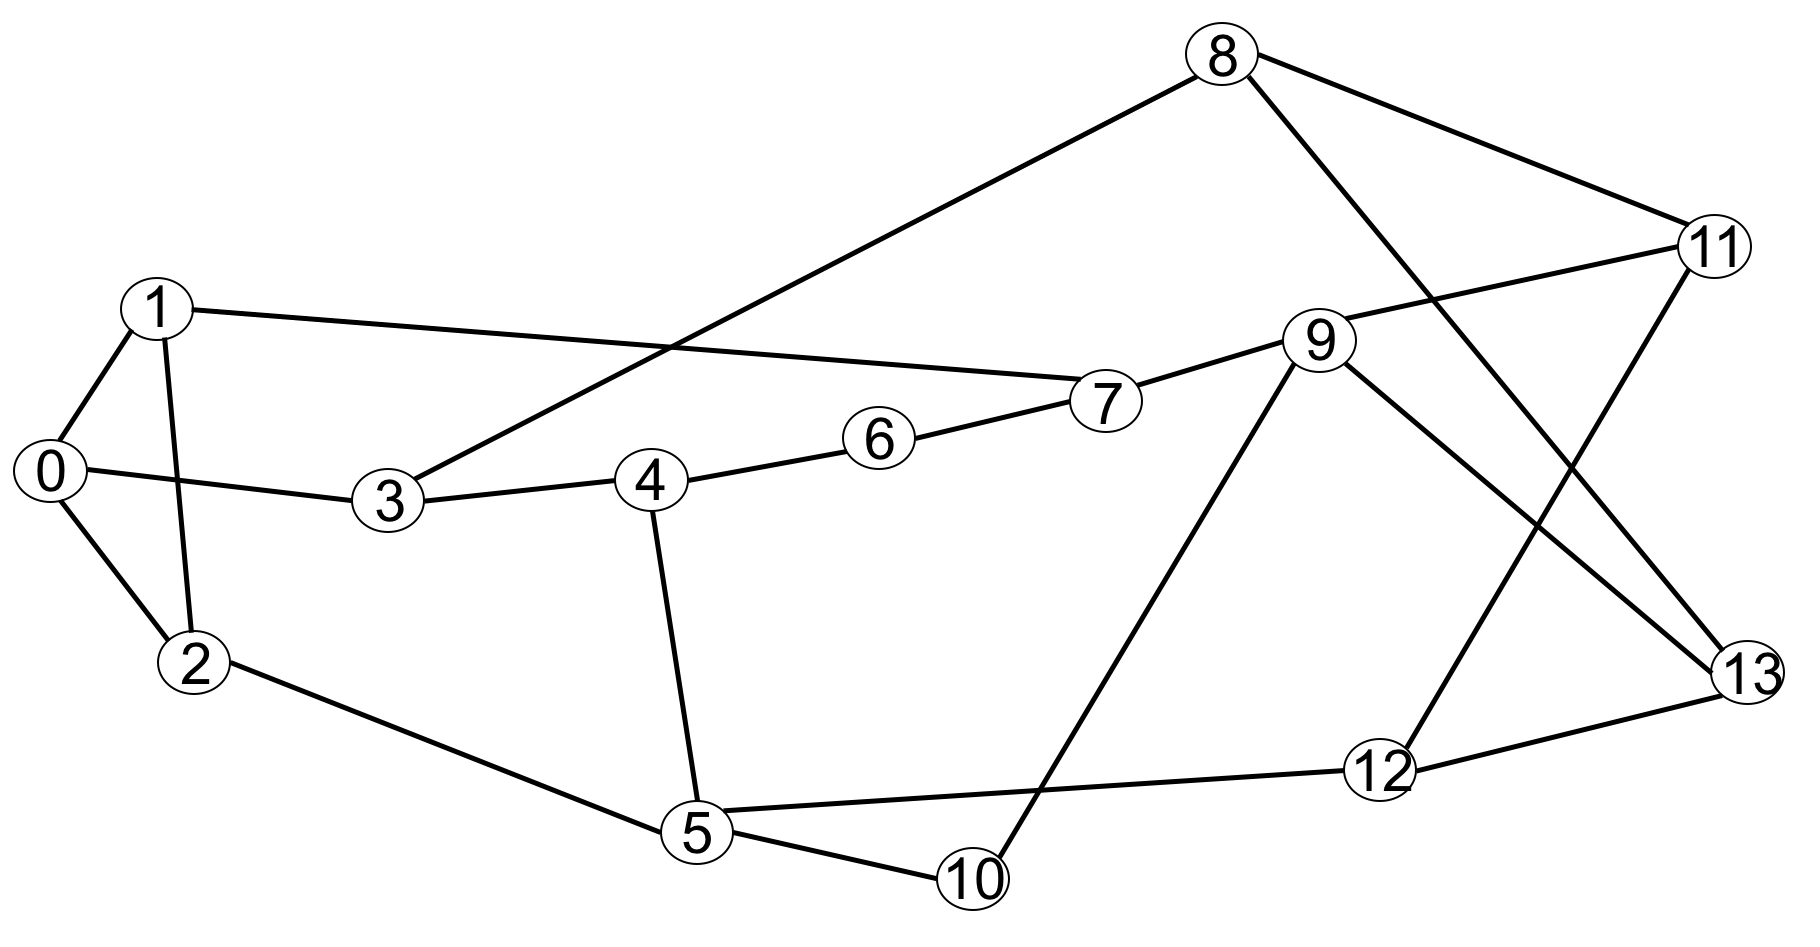
\includegraphics[scale=0.25]{figures/NSF_net.png}
    \caption{Topology of NSFNET network. Node $5$ is on the highest number of shortest paths between all pairs, so it is the bottleneck node.}
    \label{fig:NSF_net}
\end{centering}
\end{figure}

We can also determine the traffic factor for an arbitrary network like the NSFNET topology \cite{nsf_net} shown in Figure \ref{fig:NSF_net}. In cases such as this, the bottleneck may not be immediately evident, but finding it is simply a matter of using any standard shortest path algorithm to find the number of shortest paths on which a node $x$ is present, $\rho(x)$, for all nodes. Then, the bottleneck node is the node with the maximum $\rho()$ value: $b = \argmax_{x} \rho(x)$. In the NSFNET topology, node $5$ is the bottleneck with $\rho(5) = 28$. As above, the probability of each path currently being used to serve a flow is $p_f = \frac{1}{N-1} = \frac{1}{13} = 0.077$. Since this probability is close to zero, the Poisson approximation with parameter $\rho(b)*p_f = 28*0.077 \approx 2.15$ is appropriate for this traffic factor distribution:
\begin{equation*}
  f_{TF_b}(t) = e^{-2.15} \frac{2.15^t}{t!}
\end{equation*}

\section{Proof of Multiplicative Chernoff Bound}
\label{sec:chernoff_bound_proof}

The authors in \cite{mitzenmacher2005probability} prove a different bound for $0 < \eta \leq 1$.  We follow the same logic to prove the following bound for $\eta \geq 1$.

\noindent
{\bf Theorem 1:}
Let $X$ be the sum of independent Poisson trials and $\mu = \mathbb{E}[X]$.  The following bound holds for $\eta \geq 1$:
\begin{equation}
\label{eq:new_chernoff_bound}
	P( TF \geq (1 + \eta)\mu_{TF} ) \leq e^{\frac{-\eta^2}{2+\eta}\mu_{TF}}
\end{equation}

\noindent
{\bf Proof:}
First, we reiterate the following relative Chernoff Bound given in \cite{mitzenmacher2005probability}:  
For any $\eta > 0$, 
\begin{equation}
\label{eq:orig_chernoff_bound}
	P( X \geq (1 + \eta) \mu ) < ( \frac{e^\eta}{(1+\eta)^{(1+\eta)}} )^\mu
\end{equation}
Using (\ref{eq:orig_chernoff_bound}), to prove (\ref{eq:new_chernoff_bound}), we must show that the following holds for $\eta \geq 1$:
\begin{equation}
\label{eq:bound_condition}
	\frac{e^\eta}{(1+\eta)^{(1+\eta)}} \leq e^{\frac{-\eta^2}{2+\eta}}
\end{equation}
Taking the natural logarithm and rearranging, we get
\begin{equation}
	f( \eta ) = \eta - (1+\eta)\ln(1+\eta) + \frac{\eta^2}{2+\eta} \leq 0
\end{equation}
Then, the first and second derivates of $f(\eta)$ with respect to $\eta$ are
\begin{equation}
	f'( \eta ) = -\ln(1+\eta) + \frac{\eta(\eta + 4)}{(\eta+2)^2}
\end{equation}
\begin{equation}
	f''( \eta ) = -\frac{1}{1+\eta} + \frac{8}{(\eta+2)^3}
\end{equation}
Note that $f(1) = -0.053$.  Additionally, for all $\eta \geq 1$, $f'(\eta) < 0$ and $f''(\eta) < 0$.  Therefore, $f(\eta)$ is decreasing and concave down for $\eta \geq 1$.  This fact, along with the fact that $f(1) < 0$, implies that $f(\eta)$ stays negative for $\eta \geq 1$.  Hence, (\ref{eq:bound_condition}) is satisfied, completing our proof.
%Since for $\eta \geq 1$, $f''(\eta)$ is always negative, $f'(\eta)$ is monotonically decreasing in this range.  Realizing that $f'(1) < 0$, then, proves that $f'(\eta)$ is also negative when $\eta \geq 1$.  Therefore, since $f(1) < 0$ also, $f(\eta) < 0$ for all $\eta \geq 1$.
\hfill$\blacksquare$

%\section{Proof of Traffic Factor for Grid Network}
%\label{sec:grid_tf_proof}
%We outline a simple proof for determining the TF of the center node in a grid of $N$ nodes using ``Row-First, Column-Second" routing.  We give the proof for when $\sqrt{N}$ is odd, but the logic follows similarly for even values.
%Assume each node is the source of exactly one flow and that the destination is uniformly chosen from all other $N-1$ nodes.  Node $i$, then, has a $\frac{1}{N-2}$ chance of choosing each non-center node.  
%%For each source node, we can determine the number of destinations that route through the center.  We separate nodes into two categories for this counting.
%
%\begin{figure}
%\begin{centering}
%    \includegraphics[scale=0.32]{figures/TF_proof_fig_color.pdf}
%    \vspace{-4mm}
%    \caption{Sources and destinations used in proving TF for grid networks}
%    \label{fig:TF_proof_fig}
%    \vspace{-6mm}
%\end{centering}
%\end{figure}
%
%First, we consider the nodes circled in set $A$ in Figure \ref{fig:TF_proof_fig}.  
%%Through manual inspection, one can deduce that the only destination nodes in the figure that result in a path that is relayed by the center node are the two bottom nodes in the center column in the figure, marked with blue.  
%The destinations that are relayed through the center are marked in blue in the figure.
%The probability of a node in set $A$ choosing one of these destinations is $P_{A} = \frac{\frac{\sqrt{N}-1}{2}}{N-2}$.
%%Now, we can count the total number of nodes for which this probability holds.  From the figure, we can quantify the number of circled nodes, but we must also consider the reverse, i.e. imagine the figure rotated vertically, so 
%The total number of nodes falling into set $A$, including the mirror of those circled in the figure, is $N_A = \sqrt{N} \cdot (\sqrt{N}-1)$.
%Then, the contribution to the TF by nodes in set $A$ is simply the product of $P_A$ and $N_A$:
%%\begin{equation}
%	$E[TF_{A}] = \frac{\frac{\sqrt{N}-1}{2}}{N-2}  \cdot  \sqrt{N} \cdot (\sqrt{N}-1)$
%%\end{equation}
%
%%Next, we consider the nodes in the same row as the center node, which we call set $B$.  
%%Here, all destinations on the ``opposite" side of the center as well as those in the same column of the center require being routed through the center node when originating from any nodes in set $B$.  Just as above, we can relate the probability of choosing one of these destinations as 
%Similarly, for set $B$: $P_{B} = \frac{\frac{\sqrt{N}+1}{2} \cdot \sqrt{N} - 1}{N-2}$
% and $N_{B} = \frac{\sqrt{N-1}}{2}$, so the expected contribution to TF from set $B$ is
%%\begin{equation}
%	$E[TF_{B}] = \frac{\frac{\sqrt{N}+1}{2} \cdot \sqrt{N} - 1}{N-2} \cdot 2 \cdot (\frac{\sqrt{N}-1}{2})$.
%%\end{equation}
%
%Since sets $A$ and $B$ account for all non-center nodes in the network, the overall expected traffic factor is just the sum of $E[TF_A]$ and $E[TF_B]$, which simplifies to
%\begin{equation}
%	E[TF] = \frac{\sqrt{N}(N - 2) + 1}{N-2}
%\end{equation}
%which is effectively $\sqrt{N}$ for large $N$.
%\vspace{-1.5mm}



%\appendix
%\input{sections/random_explanation}
% conference papers do not normally have an appendix


% use section* for acknowledgement
%\section*{Acknowledgment}


%The authors would like to thank...


% trigger a \newpage just before the given reference
% number - used to balance the columns on the last page
% adjust value as needed - may need to be readjusted if
% the document is modified later
%\IEEEtriggeratref{8}
% The "triggered" command can be changed if desired:
%\IEEEtriggercmd{\enlargethispage{-5in}}

% references section

% can use a bibliography generated by BibTeX as a .bbl file
% BibTeX documentation can be easily obtained at:
% http://www.ctan.org/tex-archive/biblio/bibtex/contrib/doc/
% The IEEEtran BibTeX style support page is at:
% http://www.michaelshell.org/tex/ieeetran/bibtex/
%\bibliographystyle{IEEEtran}
% argument is your BibTeX string definitions and bibliography database(s)
%\bibliography{IEEEabrv,../bib/paper}
%
% <OR> manually copy in the resultant .bbl file
% set second argument of \begin to the number of references
% (used to reserve space for the reference number labels box)
%\begin{thebibliography}{1}


\bibliographystyle{unsrt}

\bibliography{references}

%\bibitem{IEEEhowto:kopka}
%H.~Kopka and P.~W. Daly, \emph{A Guide to \LaTeX}, 3rd~ed.\hskip 1em plus
%  0.5em minus 0.4em\relax Harlow, England: Addison-Wesley, 1999.

%\end{thebibliography}




% that's all folks
\end{document}


